%----------
%   WARNING
%----------

% This Guide contains Library recommendations based mainly on APA and IEEE styles, but you must always follow the guidelines of your TFG Tutor and the TFG regulations for your degree.

% THIS TEMPLATE IS BASED ON THE IEEE STYLE 


%----------
% DOCUMENT SETTINGS
%----------

\documentclass[12pt]{report} % font: 12pt

% margins: 2.5 cm top and bottom; 3 cm left and right
\usepackage[
a4paper,
vmargin=2.5cm,
hmargin=3cm
]{geometry}

% Paragraph Spacing and Line Spacing: Narrow (6 pt / 1.15 spacing) or Moderate (6 pt / 1.5 spacing)
\renewcommand{\baselinestretch}{1.15}
\parskip=6pt

% Color settings for cover and code listings 
\usepackage[table]{xcolor}
\definecolor{azulUC3M}{RGB}{0,0,102}
\definecolor{gray97}{gray}{.97}
\definecolor{gray75}{gray}{.75}
\definecolor{gray45}{gray}{.45}

\usepackage{enumerate}

% PDF/A -- Important for its inclusion in e-Archive. PDF/A is the optimal format for preservation and for the generation of metadata: http://uc3m.libguides.com/ld.php?content_id=31389625. 

% In the template we include the file OUTPUT.XMPDATA. You can download that file and include the metadata that will be incorporated into the PDF file when you compile the memoria.tex file. Then upload it back to your project.  
\usepackage[a-1b]{pdfx}

% LINKS
\usepackage{hyperref}
\hypersetup{colorlinks=true,
	linkcolor=blue, % links to parts of the document (e.g. index) in black (changed because a black link in a black text does not make any sense whatsoever)
	urlcolor=blue} % links to resources outside the document in blue

% MATH EXPRESSIONS
\usepackage{amsmath,amssymb,amsfonts,amsthm}

\newcommand*{\mynum}[1]{\num[output-decimal-marker={.},
                             round-mode=places,
                             round-precision=2,
                             group-digits=false]{#1}}

\newtheorem{definition}{Definition}
\newtheorem{theorem}{Theorem}
\newtheorem{problem}{Problem}
\newtheorem{example}{Example}
\newtheorem{corollary}{Corollary}
\newtheorem{lemma}{Lemma}
\newtheorem{remark}{Remark}


% Character encoding
\usepackage{txfonts} 
\usepackage[T1]{fontenc}
\usepackage[utf8]{inputenc}

% English settings
\usepackage[english]{babel} 
\usepackage[babel, english=american]{csquotes}
\AtBeginEnvironment{quote}{\small}

\usepackage{todonotes}
\usepackage{wrapfig}
% Footer settings
\usepackage{fancyhdr}
\pagestyle{fancy}
\fancyhf{}
\renewcommand{\headrulewidth}{0pt}
\rfoot{\thepage}
\fancypagestyle{plain}{\pagestyle{fancy}}

% DESIGN OF THE TITLES of the parts of the work (chapters and epigraphs or sub-chapters)
\usepackage{titlesec}
\usepackage{titletoc}
\titleformat{\chapter}[block]
{\large\bfseries\filcenter}
{\thechapter.}
{5pt}
{\MakeUppercase}
{}
\titlespacing{\chapter}{0pt}{0pt}{*3}
\titlecontents{chapter}
[0pt]                                               
{}
{\contentsmargin{0pt}\thecontentslabel.\enspace\uppercase}
{\contentsmargin{0pt}\uppercase}                        
{\titlerule*[.7pc]{.}\contentspage}                 

\titleformat{\section}
{\bfseries}
{\thesection.}
{5pt}
{}
\titlecontents{section}
[5pt]                                               
{}
{\contentsmargin{0pt}\thecontentslabel.\enspace}
{\contentsmargin{0pt}}
{\titlerule*[.7pc]{.}\contentspage}

\titleformat{\subsection}
{\normalsize\bfseries}
{\thesubsection.}
{5pt}
{}
\titlecontents{subsection}
[10pt]                                               
{}
{\contentsmargin{0pt}                          
	\thecontentslabel.\enspace}
{\contentsmargin{0pt}}                        
{\titlerule*[.7pc]{.}\contentspage}  


% Tables and figures settings
\usepackage{multirow} % combine cells 
\usepackage{caption} % customize the title of tables and figures
\usepackage{floatrow} % we use this package and its \ ttabbox and \ ffigbox macros to align the table and figure names according to the defined style.
\usepackage{array} % with this package we can define in the following line a new type of column for tables: custom width and centered content
\newcolumntype{P}[1]{>{\centering\arraybackslash}p{#1}}
\DeclareCaptionFormat{upper}{#1#2\uppercase{#3}\par}
\usepackage{graphicx}
\graphicspath{{imagenes/}} % Images folder

% Table layout for engineering
\captionsetup*[table]{
	format=upper,
	name=TABLE,
	justification=centering,
	labelsep=period,
	width=.75\linewidth,
	labelfont=small,
	font=small
}

% Figures layout for engineering
\captionsetup[figure]{
	format=hang,
	name=Fig.,
	singlelinecheck=off,
	labelsep=period,
	labelfont=small,
	font=small		
}

% FOOTNOTES
\usepackage{chngcntr} % continuous numbering of footnotes
\counterwithout{footnote}{chapter}

% CODE LISTINGS 
% support and styling for listings. More information in  https://es.wikibooks.org/wiki/Manual_de_LaTeX/Listados_de_código/Listados_con_listings
\usepackage{listings}

% Custom listing
\lstdefinestyle{estilo}{ frame=Ltb,
	framerule=0pt,
	aboveskip=0.5cm,
	framextopmargin=3pt,
	framexbottommargin=3pt,
	framexleftmargin=0.4cm,
	framesep=0pt,
	rulesep=.4pt,
	backgroundcolor=\color{gray97},
	rulesepcolor=\color{black},
	%
	basicstyle=\ttfamily\footnotesize,
	keywordstyle=\bfseries,
	stringstyle=\ttfamily,
	showstringspaces = false,
	commentstyle=\color{gray45},     
	%
	numbers=left,
	numbersep=15pt,
	numberstyle=\tiny,
	numberfirstline = false,
	breaklines=true,
	xleftmargin=\parindent
}

\usepackage[normalem]{ulem}
\captionsetup*[lstlisting]{font=small, labelsep=period}
 
\lstset{style=estilo}
\renewcommand{\lstlistingname}{\uppercase{Code}}


% REFERENCES 

% IEEE bibliography setup
\usepackage[backend=biber, style=ieee, isbn=false,sortcites, maxbibnames=6, minbibnames=1]{biblatex} % Setting for IEEE citation style, recommended for engineering. "maxbibnames" indicates that from 6 authors truncate the list in the first one (minbibnames) and add "et al." as used in the IEEE style.

\addbibresource{referencias.bib} % The references.bib file in which the bibliography used should be

\usepackage{graphbox}
\usepackage{rotating}
% start TeXmacs macros
\newcommand{\nobracket}{}
\newcommand{\tmmathbf}[1]{\ensuremath{\boldsymbol{#1}}}
\newcommand{\tmem}[1]{{\em #1\/}}
\newcommand{\tmop}[1]{\ensuremath{\operatorname{#1}}}
\newcommand{\tmstrong}[1]{\textbf{#1}}
\newcommand{\tmverbatim}[1]{\text{{\ttfamily{#1}}}}
\providecommand{\xequal}[2][]{\mathop{=}\limits_{#1}^{#2}}
\newcommand{\tmcolor}[2]{{\color{#1}{#2}}}
\newcommand{\mathLaplace}{\Delta}
\hfuzz=60.0pt 
% end TeXmacs macros
\usepackage{pdfpages}

%-------------
%	DOCUMENT
%-------------

\begin{document}
\pagenumbering{roman} % Roman numerals are used in the numbering of the pages preceding the body of the work.

%----------
%	COVER
%----------	
\begin{titlepage}
  \begin{sffamily}
    \color{azulUC3M}
    \begin{center}
      \begin{figure}[ht] % UC3M Logo
        \makebox[\textwidth][c]{
\includegraphics[width=16cm]{logo_UC3M.png}}
      \end{figure}
      \vspace{2.5cm}
      \begin{Large}
        Master Degree in Computational and Applied Mathematics\\
        2023-2024\\ % Academic year
        \vspace{2cm}
        \textsl{Master Thesis}
        \bigskip

      \end{Large}
      {\Huge ``An RBF-based Physics-Informed Neural Network''}\\
      \vspace*{0.5cm}
      \rule{10.5cm}{0.1mm}\\
      \vspace*{0.9cm}
      {\LARGE Héctor Rodrigo Iglesias Goldaracena}\\
      \vspace*{1cm}
      \begin{Large}
        1st Víctor Bayona Revilla\\
        2nd Pedro González Rodríguez\\
        Place and date\\
      \end{Large}
    \end{center}
    \vfill
    \color{black}
    \fbox{
      \begin{minipage}{\linewidth}
        \textbf{AVOID PLAGIARISM}\\
        \footnotesize{The University uses the \textbf{Turnitin Feedback Studio} for the delivery of student work. This program compares the originality of the work delivered by each student with millions of electronic resources and detects those parts of the text that are copied and pasted. Plagiarizing in a TFM is considered a  \textbf{\underline{Serious Misconduct}}, and may result in permanent expulsion from the University.}\end{minipage}}

    % IF OUR WORK IS TO BE PUBLISHED UNDER A CREATIVE COMMONS LICENSE, INCLUDE THESE LINES. IS THE RECOMMENDED OPTION.
    \noindent
\includegraphics[width=4.2cm]{creativecommons.png}\\ % Creative Commons Logo
    \footnotesize{This work is licensed under Creative Commons \textbf{Attribution – Non Commercial – Non Derivatives}}

  \end{sffamily}
\end{titlepage}

\newpage % blank page
\thispagestyle{empty}
\mbox{}

\newpage % blank page
\thispagestyle{empty}
\mbox{}

%----------
%	ABSTRACT AND KEYWORDS 
%----------	
\renewcommand\abstractname{\large\bfseries\filcenter\uppercase{Summary}}
\begin{abstract}
  \thispagestyle{plain}
  \setcounter{page}{3}

  % Write your abstract

  \textbf{Keywords:} % add the keywords

  \vfill
\end{abstract}
\newpage % Blank page
\thispagestyle{empty}
\mbox{}


%----------
%	Dedication
%----------	
% \chapter*{Dedication}

\setcounter{page}{5}

% Write here	

\vfill

\newpage % blank page
\thispagestyle{empty}
\mbox{}


%----------
%	TOC
%----------	

%--
% TOC
%-
\tableofcontents
\thispagestyle{fancy}

\newpage % blank page
\thispagestyle{empty}
\mbox{}

%--
% List of figures. If they are not included, comment the following lines
%-
\listoffigures
\thispagestyle{fancy}

\newpage % blank page
\thispagestyle{empty}
\mbox{}

%--
% List of tables. If they are not included, comment the following lines
%-
\listoftables
\thispagestyle{fancy}

\newpage % blankpage
\thispagestyle{empty}
\mbox{}


%----------
%	THESIS
%----------	
\clearpage
\pagenumbering{arabic} % numbering with Arabic numerals for the rest of the document.	

\chapter{Introduction}
% \section{Motivation}

Machine Learning (ML) has experienced a surge in popularity and application across various
domains in recent years, which can be owed to different contributing factors.
Firstly, the development of now readily available high performance hardware like
Graphics Processing Units (GPUs) has significantly sped up the times of training
and inference of ML models, where
repeated operations are common \cite{oh2004gpu}.
Moreover, algorithmic improvements like automatic differentiation has enabled a streamlined
way to find suitable parameters for models solving a wide variety of problems
\cite{baydin2018automatic}.

A second contributing factor is data availability. Be it social media,
embedded hardware sensors or any of our technological devices, a copious amount of data
is produced
by the minute which can then be labored by ML algorithms to identify patterns and
make predictions. Not only that, governments worldwide are fostering open access to
data across domains as varied as culture, demography, environment and technology.
In particular, the government of Spain, the country where this Master's thesis has been
written in, is undertaking efforts in the framework of their
\href{https://datos.gob.es/en}{Open Data initiative} to leverage collaboration between
analysts and contributing to the spread of knowledge.

Precisely along this last idea, the third key contributing factor is found in the form
of Free and Open Source Software (FOSS). The open nature of ML libraries like
\href{https://pytorch.org/}{PyTorch} and \href{https://www.tensorflow.org/}{TensorFlow}
have not only made state-of-the-art
techniques accessible to the broad public, but also seen the benefits entailing any FOSS
project: volunteers and professionals alike freely
contributing in a transparent environment
to the improvement, triaging, interoperability and other extensions of these projects.

Despite its widespread adoption and empirical success, a robust theoretical foundation that
guarantees the effectiveness of ML is still lacking, while empirical evidence abounds
regarding its usefulness across multiple areas of knowledge.

One notable characteristic of ML models is their inherent complexity, which often manifests
in intricate model architectures and parameter configurations \cite{cuomo2022scientific}.
The currently heuristic nature of ML techniques stands in the way of decisively
anticipating if a given model will be up to the task at hand.
Indeed, while it is true that one can always verify if the inputs of
the model suit the problem parameters and if the output of the model suits the solution,
providing a justification of the effectiveness of each intermediate layer that is
exempt of heuristics is a non-trivial task.

Drawing parallels with classical numerical methods, such as the finite element method (FEM) for
solving partial differential equations (PDEs), provides valuable insights into the underlying
principles of some models in ML. In the former framework,
basis functions are employed to
reconstruct the target function through a linear combination, akin to the linear combination
one would expect to find at the last layer of many neural networks.

However, a fundamental distinction arises in the
prescription of basis functions: while numerical methods explicitly define basis functions,
such as ``hat'' functions for solving ordinary differential equations (ODEs), ML practitioners
rely on arbitrarily complex compositions of functions which have been empirically verified
to possess sufficient approximation capacity for the desired problem domains.

Latent similarities between FEM (as well as other techniques) and ML practices
can potentially show the way forward to reconciling well-known theoretical principles with
surging empirical methodologies. While numerical
methods offer rigorous formulations and verifiable procedures, ML adopts a more heuristic
approach by leveraging compositions of functions with empirically validated approximation
capabilities.

The aim of this work is to establish an intermediary perspective that intertwines
mathematical theory, particularly that of Radial Basis Functions (RBFs), with the
computational power and flexibility supplied by ML techniques.


\section{Objectives}

\chapter{State of the art}
\section{Neural Networks} \label{sec-neural-networks}
The starting point for defining a Neural Network is the multilayer perceptron, whose recursive definition we express following \cite{lu2021deepxde}:
\begin{definition}[Multilayer perceptron]
  Let \(L \in \mathbb{N}\) and \(\{ N_i \}_{i = 1}^L \subset \mathbb{N}\). The
    {\textbf{$L-$layer perceptron}} is a function
  \begin{equation}
    \begin{array}{llll}
      \mathcal{N}^L : & \mathbb{R}^{N_0} & \rightarrow     & \mathbb{R}^{N_L}                   \\
                      & \tmmathbf{x}     & \hookrightarrow & \tmmathbf{W}^L \mathcal{N}^{L - 1}
      (\tmmathbf{x}) +\tmmathbf{b}^L
    \end{array},
    \label{perceptronRule}
  \end{equation}
  % \[ \begin{array}{llll}
  %      \mathcal{N}^L : & \mathbb{R}^{N_0} & \rightarrow & \mathbb{R}^{N_L}\\
  %      & \tmmathbf{x} & \hookrightarrow & \tmmathbf{W}^L \mathcal{N}^{L - 1}
  %      (\tmmathbf{x}) +\tmmathbf{b}^L
  %    \end{array}, \]
  where \(\mathcal{N}^{L - 1} : \mathbb{R}^{N_0} \rightarrow \mathbb{R}^{N_{L- 1}}\) is defined according to the rule
  \[ \mathcal{N}^{L - 1} (\tmmathbf{x}) = \left\{\begin{array}{ll}
      \tmmathbf{x},           & \text{if } L = 1 \\
      \sigma_{L - 1} (\tmmathbf{W}^{L - 1} \mathcal{N}^{L - 2} (\tmmathbf{x})
      +\tmmathbf{b}^{L - 1}), & \text{otherwise}
    \end{array}\right. . \]
  We shall refer to some \(\tmmathbf{b}^i \in \mathbb{R}^{\mathbb{N}_i}, 1 \leq i \leq L\) as the {\textbf{bias}} of the \(i -\)th layer, and each
  \(\tmmathbf{W}^i \in \mathbb{R}^{N_i \times N_{i - 1}}\) as the
  \textbf{weights matrix} of the \(i -\)th layer. Finally, the \textbf{activation function} of the $i
    -$th layer, \(\sigma_i\), is commonly defined as
  \[ \begin{array}{cccc}
      \sigma_i : & \mathbb{R}^{\mathbb{N}_i} & \rightarrow     &
      \mathbb{R}^{\mathbb{N}_i}                                                               \\
                 & (x_1, x_2, \ldots, x_i)   & \hookrightarrow & (\phi_i (x_1), \phi_i (x_2),
      \ldots, \phi_i (x_n))
    \end{array} \]
  that is, the element-wise application of some function
  $\phi_i$.

  The multilayer perceptron is also named \textbf{feedforward network}.
\end{definition}

Some common activation function choices are the sigmoid function, $x \mapsto 1/(1 + e^{- x})$, the hyperbolic tangent, $x \mapsto (e^x - e^{- x})/(e^x + e^{- x})$ and the Rectified Linear Unit (ReLU), $x \mapsto \max \{ 0, x \}$.

Contrary to what one may instinctively think, the $1 -$layer perceptron equipped with a suitable activation function is
enough to characterize any continuous function, that is, it is
  {\tmstrong{dense}} in the space of continuous functions of $n \text{
    variables, } C (I_n)$. We briefly quote the terminology and formulation
proposed by Cybenko in \cite{cybenko1989approximation}, where a proof of this result can be found.

\begin{definition}[Discriminatory function]
  Let $M (I_n)$ denote the space of finite, signed regular measures on \(I_n\).
  A function \(\sigma\) is said to be {\tmstrong{discriminatory}} if for a
  measure \(\mu \in M (I_n)\) we have that
  \[ \int_{I_n} \sigma (y^{\top} x + \theta) d \mu (x) = 0 \text{ for all } y
    \in \mathbb{R}^n, \theta \in \mathbb{R} \]
  implies that \(\mu = 0\).
  % Moreover, a function $t \mapsto \sigma (t)$ is said
  % to be {\tmstrong{sigmoidal}} if
  % \[ \lim_{t \rightarrow + \infty} \sigma (t) = 1, \text{ and } \lim_{t
  % \rightarrow - \infty} \sigma (t) = 0. \]
\end{definition}

\begin{theorem}[Universal approximation]
  Let \(\sigma\) be any continuous discriminatory function. Then, finite sums of
  the form
  \[ G (x) = \sum_{j = 1}^N \alpha_j \cdot \sigma (y_j^{\top} x + \theta_j) \]
  are dense in \(C (I_n)\), i.e., for any $\varepsilon > 0 \text{ and } f \in C
    (I_n)$ we can find a sum \(G (x)\) such that
  \[ | G (x) - f (x) | < \varepsilon \text{, for } x \in I_n . \]
\end{theorem}



\section[PINNs]{PINNs\footnote{Throughout this section, we shall follow the order of presentation proposed in \cite{cuomo2022scientific}.}}\label{section:pinns}

Physics-Informed Neural Networks (PINNs in the following) constitute the
machine learning techniques that are used to solve Partial Differential
Equations, which are problems of the form
\begin{equation}
  (P) = \left\{\begin{array}{rlll}
    F (u (\tmmathbf{z}) ; \gamma) & = & f (\tmmathbf{z}), & \tmmathbf{z} \in
    \Omega                                                                            \\
    B (u (\tmmathbf{z}))          & = & g (\tmmathbf{z}), & \tmmathbf{z} \in \partial
    \Omega
  \end{array}\right. \label{pdegeneralform}
\end{equation}
where we consider the open set $\Omega \subset \mathbb{R}^d$ whose boundary is
denoted $\partial \Omega$, with $\tmmathbf{z}= (\tmmathbf{x}, t)$. Moreover,
\(F\) is a non-linear differential operator whose arguments are the solution $u$
we want to find, up to some model parameters $\gamma$ and prescribed to be
equal to our problem data \(f\). Finally, \(B\) is an operator which can denote
initial (\(t = 0\)) or boundary conditions. For instance, if $B$ is set to be
the identity operator (resp., gradient operator) we recover Dirichlet (resp.,
Neumann) boundary conditions.

Provided $\gamma$ is known, the process of finding $u$ is called
  {\tmstrong{forward}} problem\footnote{We shall focus the rest of the
  discussion on problems of this form.}. Reciprocally, if $\gamma$ is to be
determined alongside $u$ up to particular measurements of the problem under study, the problem is called {\tmstrong{inverse}}. Under
the PINN framework, and denoting by $(\tmmathbf{z}, \theta) \mapsto
  \mathcal{N}\mathcal{N} (\tmmathbf{z}; \theta)$ an arbitrary neural network of input $\tmmathbf{z}$ and
parameters $\theta$, we intend to find suitable $\hat{ \theta}$ such that
$\mathcal{N}\mathcal{N} (\tmmathbf{z}; \hat{ \theta}) \simeq u (\tmmathbf{z})$. The
usual work plan involves finding
\begin{equation}
  \arg \min_{\theta} \mathcal{L} (\theta) = \arg \min_{\theta} \omega_F
  \mathcal{L}_F (\theta) + \omega_B \mathcal{L}_B (\theta),
  \label{loss-fun-pinn}
\end{equation}
where
\begin{equation}
  \mathcal{L}_F (\theta) = \int_{\Omega} (F (\mathcal{N}\mathcal{N}
  (\tmmathbf{z}; \theta)) - f (\tmmathbf{z}))^2 d\tmmathbf{z},
  \label{loss-F}
\end{equation}
and
\begin{equation}
  \mathcal{L}_B (\theta) = \int_{\partial \Omega} (B (\mathcal{N}\mathcal{N}
  (\tmmathbf{z}; \theta)) - g (\tmmathbf{z}))^2 d\tmmathbf{z}
  \label{loss-boundary}
\end{equation}
which come usually prescribed as mean square errors in the corresponding
discretized form. Finally, $\omega_F$, $\omega_B$ are weights that account for the
reliability of the PDE and how strictly we need the boundary conditions to be
satisfied, respectively.

One question that needs addressing is the computation of $F
  (\mathcal{N}\mathcal{N} (z ; \theta))$. To do so, we first briefly recall the
differentiation techniques that are often studied in undergraduate courses:
\begin{itemize}
  \item The most elementary one is simply computing them by hand. This allows
        us to obtain analytical expressions that can be directly programming into
        the code we are developing to solve some problem, which saves us the
        computation times that come from differentiating.

  \item After a course in numerical methods, {\tmstrong{finite
              differentiation}} is introduced as an easy to program alternative: it
        proposes the discretization of the problem domain, generating a point set
        with as many dimensions as required by the problem. On this set, we apply
        known formulae to approximate the derivatives of the function we intend to
        study.

        A relevant disadvantage of this method is that the grid has to be stored in memory, which poses an upper
        limit to the amount of points we can sample. Another drawback is that the finite differences method decreases its performance as the
        dimension of the problem increases. Indeed, let $f : \mathbb{R}^d
          \rightarrow \mathbb{R}$ be a differentiable function. Considering the 1-step
        forward finite difference formula for a common step $h$, its partial
        derivative $\frac{\partial f}{\partial x_i}$ is computed by evaluating $f
          (x_1, \ldots, x_i, \ldots, x_d)$ and $f (x_1, \ldots, x_i + h, \ldots,
          x_d)$. Consequently, the computation of just the first $n$ partial
        derivatives of $y$ already involves $d + 1$ computations.

  \item Finally, {\tmstrong{symbolic differentiation}} corresponds to the
        differentiation techniques proportioned by the \href{https://www.mathworks.com/help/symbolic/index.html?s\_tid=CRUX\_lftnav}{Matlab Symbolic Toolbox} or \href{https://www.sympy.org/en/index.html}{SymPy}.
        It allows the user to work with the so-called symbolic variables, which
        stand for the usual variables $x, y, z, t$ we use to define functions or
        solve equations. Symbolic differentiation of a function returns another
        function, which completely avoids the problem of numerical approximations.
        However, it is a memory intensive and slow approach.
\end{itemize}

There is a fourth method, called \textbf{automatic differentiation}. This term refers to a set of techniques that exploit the chain rule to evaluate the differential of a given function to machine precision, that is, the differential is as precise as the floating point system we are using on the computing device. This technique also stems from the fact that, in its simplest terms, computer-assisted computations feature elemental functions such as the sine or exponential, as well as elementary arithmetic operations like the sum or product \cite{verma2000introduction}.

To preserve the relevancy of the discussion, we turn to a short example for illustrating automatic differentiation using the so-called ``reverse mode'', which is present in current machine learning software packages such as PyTorch or TensorFlow.

Consider the function $f (x_1, x_2) = e^{2 x_1} - \cos (x_1 x_2)$, which we
shall apply reverse mode automatic differentiation on. This function can be
written as per the scheme in Figure \ref{fig:wengert-trace}, which is also referred to
as the Wengert trace.

\begin{figure}[ht]
  \centering
  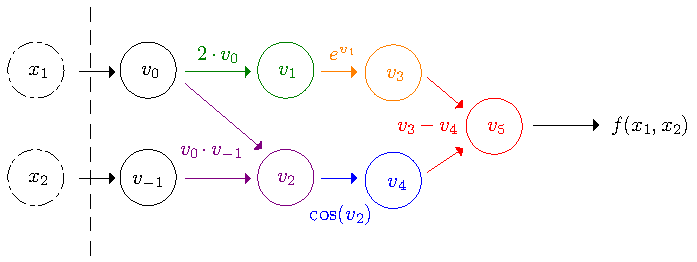
\includegraphics[width=\textwidth]{imagenes/wengert-trace.pdf}
  \caption{Wengert's trace of the function proposed as an example.}
  \label{fig:wengert-trace}
\end{figure}

Assuming that $x_1 = 2, x_2 = 3$, the evaluation of the function according to
the previous graph (i.e., evaluating from left to right) yields $v_0 = 2, v_{-
      1} = 3, v_1 = 4, v_2 = 6, v_3 \simeq 54.60, v_4 \simeq 0.96, v_5 \simeq
  53.64$. Reverse mode automatic differentiation traverses the trace in
``reverse'' order, starting off $f (x_1, x_2)$ and working our way back to
$v_0$ and $v_{- 1}$. This operation is similar to a breadth-first search,
whereby we apply the chain rule and then plug in the values we have for all
our $v$'s. If the trace is to be regarded like a tree, we can separate the
evaluation of these operations in levels:
\begin{itemize}
  \item First level
        \[ \tmcolor{red}{\frac{\partial f}{\partial v_5}} = \frac{\partial
            f}{\partial f} = 1 \]
  \item Second level
        \[ \tmcolor{orange}{\frac{\partial f}{\partial v_3}} =
          \tmcolor{red}{\frac{\partial f}{\partial v_5}} \cdot \frac{\partial
            v_5}{\partial v_3} = \tmcolor{red}{\frac{\partial f}{\partial v_5}} \cdot
          \frac{\partial (v_3 - v_4)}{\partial v_3} = 1, \quad
          \tmcolor{blue}{\frac{\partial f}{\partial v_4}} =
          \tmcolor{red}{\frac{\partial f}{\partial v_5}} \cdot \frac{\partial
            v_5}{\partial v_4} = \tmcolor{red}{\frac{\partial f}{\partial v_5}} \cdot
          \frac{\partial (v_3 - v_4)}{\partial v_4} = - 1 \]
  \item Third level
        \[ {\color[HTML]{008000}\frac{\partial f}{\partial v_1}} =
          \tmcolor{orange}{\frac{\partial f}{\partial v_3}} \cdot \frac{\partial
            v_3}{\partial v_1} = 1 \cdot \frac{\partial (e^{v_1})}{\partial v_1} =
          e^{v_1} \simeq 54.60, \quad {\color[HTML]{800080}\frac{\partial
              f}{\partial v_2}} = \tmcolor{blue}{\frac{\partial f}{\partial v_4}} \cdot
          \frac{\partial v_4}{\partial v_2} = - \frac{\partial v_4}{\partial v_2} =
          \sin (v_2) \simeq - 0.28 \]
  \item Fourth level
        \[ \frac{\partial f}{\partial v_0} = {\color[HTML]{008000}\frac{\partial
            f}{\partial v_1}} \cdot \frac{\partial v_1}{\partial v_0} +
          \frac{\partial f}{\partial v_2} \cdot \frac{\partial v_2}{\partial v_0} =
          2 e^{v_1} + \sin (v_2) \cdot v_{- 1} \simeq 110.04 \]
        \[ \frac{\partial f}{\partial v_{- 1}} = {\color[HTML]{800080}\frac{\partial
                f}{\partial v_2}} \cdot \frac{\partial v_2}{\partial v_{- 1}} = \sin
          (v_2) \cdot v_0 \simeq - 0.56 \]
\end{itemize}

As it follows from the example, we have been able to compute the differential of the function with respect to all of its variables by just traversing once the evaluation trace.

Figure \ref{fig:autodiffgraph} depicts the architectural scheme of a PINN during its training phase. Notice that it features the components present in every machine learning model's learning phase depiction (e.g., \cite{chollet2021deep}\footnote{Figure 1.9.}), but with the explicit presence of the automatic differentiation module, which allows for the computation of the loss function. For each input $\tmmathbf{z}$ and parameters $\theta$, the model generates a prediction $\mathcal{NN}(\tmmathbf{z};\theta)$ whose correctness is evaluated against our loss function $\mathcal{L}(\theta)$. Recall that the definition of the loss function comes prescribed by \eqref{loss-F} and \eqref{loss-boundary}, to be defined given a particular problem $(P)$. Because these components involve differential operators, the model is differentiated with respect to the input values by means of automatic differentiation. The parameters of the model are then updated by the action of the optimizer on the loss function. %The novelty introduced by PINNs with respect to the usual machine learning model's training phase depiction (e.g., \cite{chollet2021deep}) is the automatic differentiation mechanism, which is essential to the computation of the loss function.

We remark that the component depicted as \textit{target} in the figure is not labeled data, but simply the restrictions imposed by the PDE. This implies that the forward problem can be regarded as an unsupervised learning problem, where $(P)$ represents the prior knowledge of the phenomenon under study, to be captured by $\mathcal{L}(\theta)$. An introductory discussion on supervised and unsupervised learning can be found in \cite{chollet2021deep}\footnote{Chapter 4.}.

\begin{figure}[ht]
  \centering
  % \frame
  {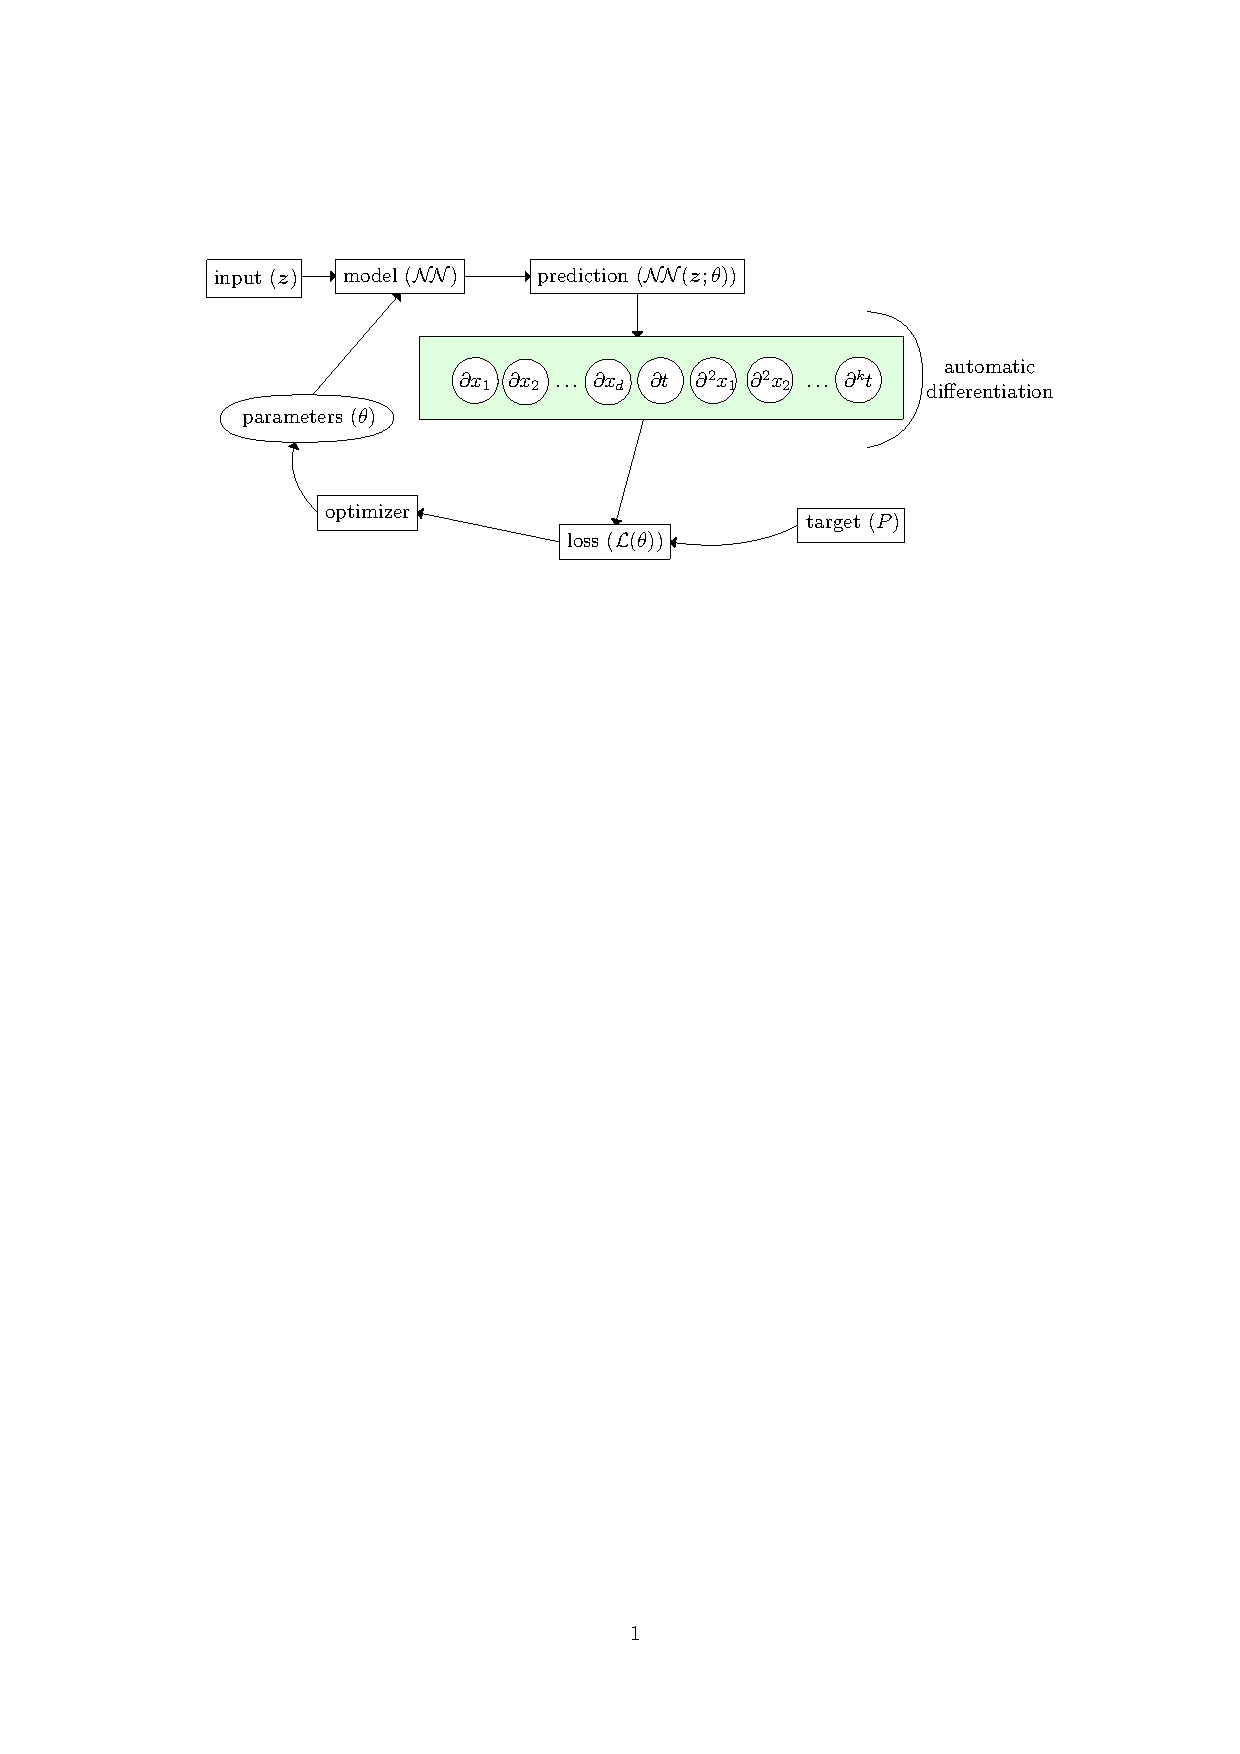
\includegraphics[width=\textwidth, clip=true, trim={3cm 20cm 3cm 4cm}]{imagenes/autodiffgraph.pdf}}
  \caption{Components of a PINN during the training phase, where we solve \eqref{loss-fun-pinn}.
  }\label{fig:autodiffgraph}
\end{figure}

\section{RBF and polynomial approximation}

% \chapter{Interpolation}

During this section, we shall present some key definitions and results
following the discussion proposed by Fasshauer \cite{fasshauer2007meshfree}.

\begin{problem}
({\tmstrong{Scattered data interpolation}}) Given $\{ (\tmmathbf{x}_j, y_j)
  \}_{j = 1}^N \subset \mathbb{R}^d \times \mathbb{R}$, find a function
$\mathcal{P}$ such that $\mathcal{P} (\tmmathbf{x}_j) = y_j$ for all $j = 1,
  \ldots, N$.\label{interpolationproblemstatement}
\end{problem}

One strategy for tackling this problem is by further assuming $\mathcal{P}$ is
a linear combination of a family of continuous basis functions $\{ \phi_j
  \}_{j = 1}^N$ on a compact metric space $\mathcal{X}$, i.e.,
\begin{equation}
  \mathcal{P} (\tmmathbf{x}) = \sum_{k = 1}^N \lambda_k \phi_k (\tmmathbf{x})
  . \label{eqn-p-is-a-linear-combination}
\end{equation}
\begin{definition}
  A function $\tmmathbf{x} \mapsto \mathcal{P} (\tmmathbf{x})$ with
  $\mathcal{P}$ as in \eqref{eqn-p-is-a-linear-combination} is called a
    {\tmstrong{generalized polynomial}}.
\end{definition}

We would then be tasked to find $\lambda_1, \ldots, \lambda_N \in \mathbb{R}$
such that
\[ \sum_{k = 1}^N \lambda_k \phi_k (\tmmathbf{x}_1) =\tmmathbf{y}_1, \sum_{k =
    1}^N \lambda_k \phi_k (\tmmathbf{x}_2) =\tmmathbf{y}_2, \ldots, \sum_{k =
    1}^N \lambda_k \phi_k (\tmmathbf{x}_N) =\tmmathbf{y}_N . \]
Note the scalar products
\[ \left\{\begin{array}{cll}
    \left(\begin{array}{ccc}
              \lambda_1 & \cdots & \lambda_N
            \end{array}\right) \left(\begin{array}{ccc}
                                     \phi_1 (\tmmathbf{x}_1) & \cdots & \phi_N (\tmmathbf{x}_1)
                                   \end{array}\right)^{\top} & = & \tmmathbf{y}_1 \\
    \left(\begin{array}{ccc}
              \lambda_1 & \cdots & \lambda_N
            \end{array}\right) \left(\begin{array}{ccc}
                                     \phi_1 (\tmmathbf{x}_2) & \cdots & \phi_N (\tmmathbf{x}_2)
                                   \end{array}\right)^{\top} & = & \tmmathbf{y}_2 \\
    \vdots                                                      &   &                         \\
    \left(\begin{array}{ccc}
              \lambda_1 & \cdots & \lambda_N
            \end{array}\right) \left(\begin{array}{ccc}
                                     \phi_1 (\tmmathbf{x}_N) & \cdots & \phi_N (\tmmathbf{x}_N)
                                   \end{array}\right)^{\top} & = & \tmmathbf{y}_N
  \end{array}\right. . \]
This system induces the system of linear equations
\begin{equation}
  \left(\begin{array}{cccc}
      \phi_1 (\tmmathbf{x}_1) & \phi_2 (\tmmathbf{x}_1) & \cdots & \phi_N
      (\tmmathbf{x}_1)                                                    \\
      \phi_1 (\tmmathbf{x}_2) & \phi_2 (\tmmathbf{x}_2) & \cdots & \phi_N
      (\tmmathbf{x}_2)                                                    \\
      \vdots                  & \vdots                  &        & \vdots \\
      \phi_1 (\tmmathbf{x}_N) & \phi_2 (\tmmathbf{x}_N) & \cdots & \phi_N
      (\tmmathbf{x}_N)
    \end{array}\right) \left(\begin{array}{c}
      \lambda_1 \\
      \lambda_2 \\
      \vdots    \\
      \lambda_N
    \end{array}\right) = \left(\begin{array}{c}
      \tmmathbf{y}_1 \\
      \tmmathbf{y}_2 \\
      \vdots         \\
      \tmmathbf{y}_N
    \end{array}\right) \label{linear-system-equations-generalized-poly}
\end{equation}
which follows the familiar form
\begin{equation}
  A \underline{\lambda} = y \label{matrixexpression-interpolationprob} .
\end{equation}
\begin{definition}
  The matrix $A$ in formulation \eqref{matrixexpression-interpolationprob} is said to
  be the {\tmstrong{interpolation matrix}}.
\end{definition}

\begin{definition}
  Under the hypotheses of Problem \ref{interpolationproblemstatement}, and
  further assuming \eqref{eqn-p-is-a-linear-combination}, we will say that the problem is
    {\tmstrong{well-posed}} (i.e., there is a unique solution to the problem) if
  and only if $A$ is non-singular.
\end{definition}


We shall now present some broadly stated results that can be found in Cheney \cite{cheney1966introduction}:

\begin{theorem}
  (Existence of the best approximations in a metric space). Let $K$ denote a
  compact set in a metric space $\mathcal{X}$. Then, for every $p \in
    \mathcal{X}$ there corresponds
  \[ k^{\ast} = \arg \min_{k \in K} d (p, k), \]
  where $d$ is the distance on $\mathcal{X}$.
\end{theorem}

This statement may (mis)lead us into only regarding $p$ and $k$ as points in
a Euclidean space. On the contrary, recall that any two functions $f, g \in
  L^p (\Omega)$ with $\Omega$ a bounded set, are also governed by the previous
theorem by setting $d (f, g) = \| f - g \|_{L^p}$, where $\| \cdot \|_{L^p}$
denotes the $L^p -$norm. Profound yet manageable results on generalized
polynomials can be given by further requesting them to satisfy the Haar
condition.

\begin{definition}
  The family of functions $\{ \phi_j \}_{j = 1}^N$ of Problem
  \ref{interpolationproblemstatement} is said to satisfy the {\tmstrong{Haar
        condition}} if every set of $N$ vectors of the form $\hat{\tmmathbf{x}} =
    (\phi_1 (\tmmathbf{x}), \phi_2 (\tmmathbf{x}), \ldots, \phi_N
    (\tmmathbf{x}))$ is linearly independent. The finite-dimensional linear function space induced by $\{ \phi_j \}_{j = 1}^N$ is said to be a {\tmstrong{Haar
        space}}.
\end{definition}

The property of linear independence can alternatively be expressed by
considering any $N$ distinct points  \{$\tmmathbf{x}_1, \ldots,
  \tmmathbf{x}_N$\}  and checking that
\[ \text{det}  [\hat{\tmmathbf{x}}_1, \hat{\tmmathbf{x}}_2, \ldots,
    \hat{\tmmathbf{x}}_n] = \left|\begin{array}{cccc}
    \phi_1 (\tmmathbf{x}_1) & \phi_2 (\tmmathbf{x}_1) & \cdots & \phi_N
    (\tmmathbf{x}_1)                                                    \\
    \phi_1 (\tmmathbf{x}_2) & \phi_2 (\tmmathbf{x}_2) & \cdots & \phi_N
    (\tmmathbf{x}_2)                                                    \\
    \vdots                  & \vdots                  &        & \vdots \\
    \phi_1 (\tmmathbf{x}_N) & \phi_2 (\tmmathbf{x}_N) & \cdots & \phi_N
    (\tmmathbf{x}_N)
  \end{array}\right| \neq 0. \]
Provided the Haar condition is satisfied,
\eqref{linear-system-equations-generalized-poly} features a unique solution.

In the case $\{ x_1, \ldots, x_N \} \subset \mathbb{R}$, we know that problem
\ref{interpolationproblemstatement} can be solved considering a polynomial of
degree $N - 1$. One could (mistakenly) venture that a similar result would be devolved for
higher dimensions, considering multivariate polynomials of degree $N-1$.

\begin{theorem}\label{thm-haar-spaces-polynomials}
  Let $\Omega \subset \mathbb{R}^d, d \geq 2$. If $\Omega$ contains an
  interior point, then there exist no Haar spaces of continuous functions except for one-dimensional ones.
\end{theorem}

\begin{proof}
  Consider any distinct $\{ \tmmathbf{x}_1, \ldots, \tmmathbf{x}_N \} \subset
    \mathbb{R}^d$ and construct the matrix $A$ as in
  \eqref{matrixexpression-interpolationprob}. If the Haar condition were
  satisfied, then $\text{det} (A) \neq 0$. Now, note that $$\text{det}
    [\hat{\tmmathbf{x}}_1, \hat{\tmmathbf{x}}_2, \ldots, \hat{\tmmathbf{x}}_n] =
    - \text{det} [\hat{\tmmathbf{x}}_2, \hat{\tmmathbf{x}}_1, \ldots,
      \hat{\tmmathbf{x}}_n].$$ Because $\Omega$ contains an interior point, we may
  consider a closed path that connects exclusively $\tmmathbf{x}_1$ and
  $\tmmathbf{x}_2$\footnote{Indeed, this path would be of measure zero in
    $\Omega$. Consequently, it can be defined to not contain $\tmmathbf{x}_3,
      \tmmathbf{x}_4, \ldots, \tmmathbf{x}_N$ along its traversal.}. We now
  continuously exchange the positions of $\tmmathbf{x}_1$ and
  $\tmmathbf{x}_2$, whereby the sign of the determinant has changed
  at its conclusion. This exchange is a continuous function of $\tmmathbf{x}_1$
  and $\tmmathbf{x}_2$. Consequently, the determinant has been zero along some
  point of the path, which is a contradiction. Note that, because the path is
  closed, the exchange function can be chosen so that we do not have
  $\tmmathbf{x}_1 = \tmmathbf{x}_2$ at any point of the exchange.
\end{proof}

Consequently, if we want to solve interpolate for a well-posed problem, it will not suffice to solve for a pre-fixed generalized polynomial. We can proceed instead by establishing a ``dependence of the basis with respect to the input data''. One possible path for doing so is considering \textbf{Radial Basis Functions}.

\begin{definition}\label{radialfunctions}
  A function $\phi : \mathbb{R}^d \rightarrow \mathbb{R}$ is said to be
    {\tmstrong{radial}} if there exists some univariate function $\varphi$ such
  that $\phi (\tmmathbf{x}) = \varphi (\| \tmmathbf{x} \|)$, where $\| \cdot
    \|$ is a norm on $\mathbb{R}^d$.
\end{definition}

The {\tmem{radial}} adjective stems from the fact that
\[ \| \tmmathbf{x}_1 \| = \| \tmmathbf{x}_2 \| \Rightarrow \varphi (\|
  \tmmathbf{x}_1 \|) = \varphi (\| \tmmathbf{x}_2 \|) \Rightarrow \phi
  (\tmmathbf{x}_1) = \phi (\tmmathbf{x}_2), \quad \forall \tmmathbf{x}_1,
  \tmmathbf{x}_2 \in \mathbb{R}^d . \]
That is, $\phi$ is radially symmetric about its center.

Furthermore, characterization in definition \ref{radialfunctions} implies that the scattered data interpolation problem can be expressed in terms of univariate functions of a given norm.
This implies that \eqref{eqn-p-is-a-linear-combination} is further refined into an
expression of the form
\begin{equation}
  \mathcal{P} (\tmmathbf{x}) = \sum_{k = 1}^N \lambda_k \varphi (\|
  \tmmathbf{x}-\tmmathbf{x}_k \|_2), \quad \tmmathbf{x} \in \mathbb{R}^d,
  \label{eqn-p-is-a-linear-combination-of-rbfs}
\end{equation}
where $\tmmathbf{x}_k$ are usually referred to as \textbf{centers}. This ultimately reshapes \eqref{linear-system-equations-generalized-poly} into
\begin{equation}
  \left(\begin{array}{cccc}
      \varphi (\| \tmmathbf{x}_1 -\tmmathbf{x}_1 \|_2) & \varphi (\|
      \tmmathbf{x}_1 -\tmmathbf{x}_2 \|_2)             & \ldots      & \varphi (\| \tmmathbf{x}_1
      -\tmmathbf{x}_N \|_2)                                                                                \\
      \varphi (\| \tmmathbf{x}_2 -\tmmathbf{x}_1 \|_2) & \varphi (\|
      \tmmathbf{x}_2 -\tmmathbf{x}_2 \|_2)             & \ldots      & \varphi (\| \tmmathbf{x}_2
      -\tmmathbf{x}_2 \|_2)                                                                                \\
      \vdots                                           & \vdots      & \ddots                     & \vdots \\
      \varphi (\| \tmmathbf{x}_N -\tmmathbf{x}_1 \|_2) & \varphi (\|
      \tmmathbf{x}_N -\tmmathbf{x}_2 \|_2)             & \ldots      & \varphi (\| \tmmathbf{x}_N
      -\tmmathbf{x}_N \|_2)
    \end{array}\right) \left(\begin{array}{c}
      \lambda_1 \\
      \lambda_2 \\
      \vdots    \\
      \lambda_N
    \end{array}\right) = \left(\begin{array}{c}
      f (\tmmathbf{x}_1) \\
      f (\tmmathbf{x}_2) \\
      \vdots             \\
      f (\tmmathbf{x}_N)
    \end{array}\right).
  \label{eqn-linear-system-equations-rbf}
\end{equation}

In the case where the problem is overdetermined (that is, we consider more data
points than centers), the matrix $A$ is no longer square (say, now $A \in
  \mathbb{R}^{m \times n}$). In such case, we come up against a linear optimization
problem where we try to find some suitable set of parameters, say $\lambda$,
such that $\| A \lambda - f \|_2$ is minimum. The solution to this problem is
then given by all $\hat{\lambda} \in \mathbb{R}^n$ satisfying the normal
equations,
\begin{equation}
  (A^{\top} A) \hat{\lambda} = A^{\top} f \label{eqn-normal-equation} .
\end{equation}
Indeed, note that
\[ \| A \lambda - f \|_2^2 = (A \lambda - f)^{\top} (A \lambda - f) =
  \lambda^{\top} (A^{\top} A \lambda - 2 A^{\top} f) + f^{\top} f. \]
Now, we differentiate with respect to the $i -$th entry of $\lambda$, which
yields
\[ e_i^{\top} (A^{\top} A \lambda - 2 A^{\top} f) + \lambda^{\top} (A^{\top} A
  e_i) = 2 e_i^{\top} (A^{\top} A \lambda - A^{\top} f), \]
where $e_i$ denotes the vector who is identically zero except for its $i -$th
entry, with value $1$. Finally,
\[ 2 e_i^{\top} (A^{\top} A \lambda - A^{\top} f) = 0 \Leftrightarrow
  A^{\top} A \lambda - A^{\top} f = 0 \Leftrightarrow (A^{\top} A) \lambda =
  A^{\top} f, \]
which is exactly \eqref{eqn-normal-equation}. Note that $A^{\top} A \in
  \mathbb{R}^{n \times n}$, which may or may not be invertible. Regardless, we
can find $\hat{\lambda}$ taking the Moore-Penrose pseudo-inverse of $A$,
presented in the following.

\begin{definition}
  Let $A \in \mathbb{R}^{m \times n}$. Then, we define the
    {\tmstrong{Moore-Penrose pseudo-inverse}}, $A^{\dag}$, as
  \[ A^{\dag} = \lim_{\varepsilon \rightarrow 0} (A^{\top} A + \varepsilon
    I_n)^{- 1} A^{\top} . \]
\end{definition}

Now, observe that \eqref{eqn-normal-equation} can be rewritten as
\[ \lim_{\varepsilon \rightarrow 0} (A^{\top} A + \varepsilon I_n)
  \hat{\lambda} = A^{\top} f. \]
Multiplying by $(A^{\top} A + \varepsilon I_n)^{- 1}$ on both sides of the
equality, we have
\[ \lim_{\varepsilon \rightarrow 0} (A^{\top} A + \varepsilon I_n)^{- 1}
  (A^{\top} A + \varepsilon I_n) \hat{\lambda} = \lim_{\varepsilon
    \rightarrow 0} (A^{\top} A + \varepsilon I_n)^{- 1} A^{\top} f \Rightarrow
  \hat{\lambda} = A^{\dag} f. \]
Indeed, even if the matrix for the overdetermined problem is not invertible
(that is, we are not using any of the soon-to-be-presented radial basis
functions), we can still find minimizers of the scattered interpolation
problem in the least squares sense.


\begin{definition}
  A real symmetric matrix $A \in \mathbb{R}^{n \times n}$ is called
    {\tmstrong{positive semi-definite}} if $\tmmathbf{x}^{\top} A\tmmathbf{x}
    \geq 0$ for all $\tmmathbf{x} \in \mathbb{R}^n$. In the case the equality
  holds if and only if $\tmmathbf{x}= 0$, we say that $A$ is
    {\tmstrong{positive definite}}.
\end{definition}

Note that if $A$ is positive semi-definite, all its eigenvalues are positive.
Indeed, if $x$ is an eigenvector of $A$ associated to an eigenvalue $\lambda$,
we have $0 < x^{\top} A x = \lambda x^{\top} x$, and because $x^{\top} x$ is
the Euclidean inner product involving non-zero vectors, we conclude $\lambda >
  0$. This implies that a positive definite matrix is non-singular.

It would be ideal for our purposes to construct positive-definite
interpolation matrices. That way, $\eqref{eqn-linear-system-equations-rbf}$ would
be well-posed.

\begin{definition}\label{def-positive-definite-functions}
  A function $\phi : \mathbb{R}^d \rightarrow \mathbb{C}$ is called
    {\tmstrong{positive definite}} on $\mathbb{R}^d$ if
  \begin{equation}
    \sum_{j = 1}^N \sum_{k = 1}^N c_j \overline{c_k} \phi (\tmmathbf{x}_j
    -\tmmathbf{x}_k) \geq 0 \label{positivedefinitefunctioncomplexdefinition}
  \end{equation}
  for any pairwise different points $\tmmathbf{x}_1, \ldots, \tmmathbf{x}_N
    \in \mathbb{R}^d$ and $\tmmathbf{c}= (c_1, \ldots, c_N)^{\top} \in
    \mathbb{C}^N$. In the case the equality holds if an only if $\tmmathbf{c}=
    0$, we shall say that $\phi$ is {\tmstrong{strictly positive definite}}.
\end{definition}

\begin{example}
  \label{funexampleutil}For a fixed $\tmmathbf{y} \in \mathbb{R}^d$, define
  $\phi (\tmmathbf{x}) = e^{i\tmmathbf{x} \cdot \tmmathbf{y}}$, where
  $\tmmathbf{x} \cdot \tmmathbf{y}$ denotes the inner product. Then, for any
  $\tmmathbf{c}= (c_1, \ldots, c_N)^{\top} \in \mathbb{C}^N$, we have
  \[ \begin{array}{ccc}
      \sum_{j = 1}^N \sum_{k = 1}^N c_j \overline{c_k} \phi (\tmmathbf{x}_j
      -\tmmathbf{x}_k) & = & \sum_{j = 1}^N \sum_{k = 1}^N c_j \overline{c_k}
      e^{i (\tmmathbf{x}_j -\tmmathbf{x}_k) \cdot \tmmathbf{y}}                        \\
                       & = & \sum_{j = 1}^N \sum_{k = 1}^N c_j \overline{c_k}
      e^{i\tmmathbf{x}_j \cdot \tmmathbf{y}- i\tmmathbf{x}_k \cdot
      \tmmathbf{y}}                                                                    \\
                       & = & \sum_{j = 1}^N c_j e^{i\tmmathbf{x}_j \cdot \tmmathbf{y}}
      \sum_{k = 1}^N \overline{c_k} e^{- i\tmmathbf{x}_k \cdot \tmmathbf{y}}
      .
    \end{array} \]
  For each $j = 1, \ldots, N$, we have that the conjugate of $c_j
    e^{i\tmmathbf{x}_j \cdot \tmmathbf{y}}$ is $\overline{c_k} e^{-
        i\tmmathbf{x}_k \cdot \tmmathbf{y}}$. Therefore,
  \begin{equation}
    \sum_{j = 1}^N \sum_{k = 1}^N c_j \overline{c_k} \phi (\tmmathbf{x}_j
    -\tmmathbf{x}_k) = \left| \sum_{j = 1}^N c_j e^{i\tmmathbf{x}_j \cdot
        \tmmathbf{y}} \right|^2 \geq 0 \label{positivedefinitepropertyasmodulus}
  \end{equation}
  and $\phi$ is positive definite.
\end{example}

\begin{theorem}
  Let $\phi_1, \ldots, \phi_N$ be positive definite functions on
  $\mathbb{R}^d$ and $c_j \geq 0$ for $j = 1, \ldots, N$. We consider their
  finite linear combination,
  \begin{equation}
    \phi (\tmmathbf{x}) = \sum_{j = 1}^N c_j \phi_j (\tmmathbf{x}), \quad
    \tmmathbf{x} \in \mathbb{R}^d . \label{linearcombinationofpsdf}
  \end{equation}
  Then, we have that
  \begin{enumerate}
    \item $\phi$ is positive definite. Moreover, it is enough that one of the
          $\phi_j$'s is strictly positive definite (with $c_j > 0$) for $\phi$ to be
          strictly positive definite.

    \item $\phi (\tmmathbf{0}) \geq 0$.

    \item \label{propevennes}$\phi (-\tmmathbf{x}) = \overline{\phi
              (\tmmathbf{x})}$.

    \item $| \phi (\tmmathbf{x}) | \leq \phi (\tmmathbf{0})$. In fact, any
          positive definite function is bounded.

    \item $\phi$ positive definite with $\phi (\tmmathbf{0}) = 0 \Rightarrow
            \phi \equiv 0$.

    \item The product of (strictly) positive definite functions is (strictly)
          positive definite functions.
  \end{enumerate}
\end{theorem}

Note that in the case that $\phi$ is a real function, property
\eqref{propevennes} implies that $\phi$ is even. In fact, this allows us to
characterize positive-definite real-valued continuous functions.

\begin{theorem}
  A real-valued continuous function $\phi$ is {\tmstrong{positive definite}}
  on $\mathbb{R}^d$ if and only if it is even and
  \[ \sum_{j = 1}^N \sum_{k = 1}^N c_j c_k \phi (\tmmathbf{x}_j
    -\tmmathbf{x}_k) \geq 0 \]
  for any pairwise different points $\tmmathbf{x}_1, \ldots, \tmmathbf{x}_N
    \in \mathbb{R}^d$ and $\tmmathbf{c}= (c_1, \ldots, c_N)^{\top} \in
    \mathbb{C}^N$. In the case the equality holds if and only if $\tmmathbf{c}=
    0$, $\phi$ is {\tmstrong{strictly positive definite}}.
\end{theorem}

\begin{theorem}\label{tm-bochner}
  ({\tmstrong{Bochner}}) A continuous function $\phi : \mathbb{R}^d
    \rightarrow \mathbb{C}$ is positive definite on $\mathbb{R}^d$ if and only
  if it is the Fourier transform of a finite Borel measure $\mu$
  on $\mathbb{R}^d$, that is, if
  \begin{equation}
    \phi (\tmmathbf{x}) = \frac{1}{\sqrt{(2 \pi)^d}} \int_{\mathbb{R}^d} e^{-
        i\tmmathbf{x} \cdot \tmmathbf{y}} d \mu (\tmmathbf{y}), \quad \tmmathbf{x}
    \in \mathbb{R}^d . \label{characterizationphitransform}
  \end{equation}
\end{theorem}

From a strategic point of view, we actually only need to prove the direction of the characterization yielding that $\phi$ is positive definite. This is the case where we assume \eqref{characterizationphitransform}. Moreover, recall that a Borel measure is one whose domain of application is the $\sigma-$algebra of Borel sets, that is, the smallest $\sigma-$algebra containing all open sets of a given topological space, $(X,\tau)$.

\begin{proof}
  Applying definition \eqref{positivedefinitefunctioncomplexdefinition}, we
  have that
  \[ \begin{array}{ccc}
      \sum_{j = 1}^N \sum_{k = 1}^N c_j \overline{c_k} \phi (\tmmathbf{x}_j
      -\tmmathbf{x}_k)                                       &
      \xequal[\text{\eqref{characterizationphitransform}}]{} &
      \frac{1}{\sqrt{(2 \pi)^d}} \sum_{j = 1}^N \sum_{k = 1}^N \left[ c_j
        \overline{c_k} \int_{\mathbb{R}^d} e^{- i (\tmmathbf{x}_j
      -\tmmathbf{x}_k) \cdot \tmmathbf{y}} d \mu (\tmmathbf{y}) \right]                                                                                 \\
      \text{(linearity of integral)}                         & =                                                           & \frac{1}{\sqrt{(2 \pi)^d}}
      \int_{\mathbb{R}^d} \left[ \sum_{j = 1}^N c_j e^{- i\tmmathbf{x}_j
            \cdot \tmmathbf{y}} \sum_{k = 1}^N \overline{c_k} e^{i\tmmathbf{x}_k
      \cdot \tmmathbf{y}} \right] d \mu (\tmmathbf{y})                                                                                                  \\
                                                             & \xequal[\text{\eqref{positivedefinitepropertyasmodulus}}]{} &
      \frac{1}{\sqrt{(2 \pi)^d}} \int_{\mathbb{R}^d} \left| \sum_{j = 1}^N
      c_j e^{- i\tmmathbf{x}_j \cdot \tmmathbf{y}} \right|^2 d \mu
      (\tmmathbf{y})                                                                                                                                    \\
                                                             & \geq                                                        & 0.
    \end{array} \]
  The inequality holds due to the non-negativity of the Borel measure.
\end{proof}

A direct consequence of this Theorem is that the function proposed in Example
\ref{funexampleutil} deserves special interest, for any other positive
definite function can be defined in terms of (infinite) linear combinations of
it, which is a more surprising result that linear combinations of the form
\eqref{linearcombinationofpsdf} resulting in (some) positive definite
function.

Even though Theorem \ref{tm-bochner} highlights the relevance
of the Gaussian function, its application is not straightforward
for deciding the positive definiteness of a function.
We shall garner more specialized tools in the following.
To this end, we first take a step back and define some key building blocks: we
start out following the presentation in {\cite{titchmarsh1939theory}}:

\begin{definition}
  Let $\varnothing = \Omega \subset \mathbb{C}$ be an open set. A function $g
    : \Omega \rightarrow \mathbb{C}$ is said to be {\tmstrong{analytic}} in $a
    \in \Omega$ if there is a power series centered in $a$ with radius $R > 0$
  such that
  \begin{equation}
    g (z) = \sum_{n = 0}^{\infty} a_n (z - a)^n
    \label{analyticasseriedepotencia}, \text{ with } | z - a | < \rho .
  \end{equation}
  That is, $g$ coincides with a power series in a neighborhood of $a$.
  Moreover, $g$ is said to be {\tmstrong{analytic}} in $\Omega$ if it is
  analytic for every $a \in \Omega$.
\end{definition}

Note that $g (a) = 0 \Rightarrow a_0 = 0$. In fact, some other coefficients
$a_1, a_2, \ldots$ may be zero. Furthermore, if $a_n = 0$ for all $n < m \in
  \mathbb{N}$ and $a_m \neq 0$, we say $g$ to have a {\tmstrong{zero of the}} $m
  -${\tmstrong{th order}}. In such case, we also have
\[ g (a) = g' (a) = \cdots = g^{m - 1} (a) = 0, \text{ and } g^m (a) \neq 0,
\]
which is clear due to \eqref{analyticasseriedepotencia}.

\begin{theorem}
  \label{theorem-titschmarch}Let $z \mapsto g (z)$ be an analytic function in
  a region $S$, and let $s_1, s_2, \ldots, s_n, \ldots$ be a set of points
  whose point of accumulation is some $s \in S$. If $g (s_i) = 0$ for every $i
    \in \mathbb{N}$, then $g (z) = 0$ for all $z \in S$.
\end{theorem}

\begin{proof}
  Because $g$ is analytic in a region $S$, identity
  \eqref{analyticasseriedepotencia} applies. Without loss of generality, we
  assume that our point of accumulation $s = a = 0$, which implies $g (z) =
    \sum_{n = 0}^{\infty} a_n z^n$ for some radius $R > 0$. To show that $g (z)
    = 0$ for all $z \in S$, we only need to show that every coefficient in
  \eqref{analyticasseriedepotencia} is zero. If that were not the case, we
  would have
  \[ g (z) = \sum_{n = k}^{\infty} a_n z^n = z^k (a_k + a_{k + 1} z + \cdots),
    \text{ for all } 0 < \rho < R. \]
  In such case, the series $\sum_{n = k}^{\infty} a_n \rho^n$ is convergent,
  which implies that each $a_n \rho^n$ is bounded, so $| a_n | \rho^n \leq K$
  for some $K$. Hence,
  \[ | g (z) | \geq | z |^k \left( | a_k | - \frac{K | z |}{\rho^{k + 1}} -
    \frac{K | z |^2}{\rho^{k + 2}} - \cdots \right) = | z |^k \left( | a_k |
    - \frac{K | z |}{\rho^k (\rho - | z |)} \right) . \]
  Because $| a_k |$ is fixed, we can make the right-hand side of the
  inequality strictly positive by taking $| z |$ sufficiently small (but not
  equal to zero). This is a contradiction with the assumption that $s = 0$ is
  an accumulation point: actually, every coefficient in $\sum_{n = 0}^{\infty}
    a_n z^n$ needs to vanish, which allows us to conclude $g (z) = 0$ for every
  $z \in S$.
\end{proof}

The following two lemmas are as formulated in {\cite{cheneylight2009course}}.

\begin{lemma}
  \label{lemma-linearly-independent-set-featuring-accumulation}Let $\{
    \lambda_j \}_{i = 1}^N$ be a set of distinct complex numbers. Then, $\{
    e^{\lambda_j z} \}_{i = 1}^N$ is a linearly independent set on any domain in
  $\mathbb{C}$ featuring a point of accumulation.
\end{lemma}

\begin{proof}
  We show the result by induction, first noting that $z \mapsto e^{\lambda_1
        z}$ is nonzero for any $z \in \mathbb{C}$. Assuming the result holds for
  some $N \in \mathbb{N}$, we define $g (z) = \sum_{j = 1}^{N + 1} c_j e^{-
        \lambda_j z}$ and assume that $g (z) = 0$ for some $z \in S \subset
    \mathbb{C}$, where $S$ has a point of accumulation. Because $g$ is an entire
  function, it follows that $g (z) = 0$ for all $z \in \mathbb{C}$. Now, we
  define
  \[ F (z) = \frac{d}{d z} (e^{- \lambda_{N + 1} z} g (z)) = \frac{d}{d z}
    \left( \sum_{j = 1}^{N + 1} c_j e^{(\lambda_j - \lambda_{N + 1}) z}
    \right) = \]
  \[ = \frac{d}{d z} \left( \sum_{j = 1}^N c_j e^{(\lambda_j - \lambda_{N +
            1}) z} + c_{N + 1} \right) = \sum_{j = 1}^N c_j (\lambda_j - \lambda_{N +
      1}) e^{(\lambda_j - \lambda_{N + 1}) z} . \]
  Because $g (z) = 0$ for all $z \in \mathbb{C}$, we have that $F \equiv 0$
  too. Applying the induction hypothesis to the set of $\{ \lambda_j -
    \lambda_{N + 1} \}_{j = 1}^N$ distinct complex numbers, we obtain that $\{
    e^{(\lambda_j - \lambda_{N + 1}) z} \}_{j = 1}^N$ is a linearly independent
  set on $S$. Therefore, $c_j (\lambda_j - \lambda_{N + 1}) = 0$ for all $j =
    1, \ldots, N$, which ultimately implies $c_j = 0$ because we assumed
  $\lambda_j \neq \lambda_{N + 1}$. Hence, $g (z) = c_{N + 1} e^{- \lambda_{N
          + 1} z} = 0$ for all $z \in \mathbb{C}$, which yields $c_{N + 1} = 0$ too.
  Consequently, $\{ e^{\lambda_j z} \}_{i = 1}^{N + 1}$ is linearly
  independent on $S$ as well.
\end{proof}

\begin{lemma}
  \label{lemma-no-accumulation-point}Let $\{ \lambda_j \}_{i = 1}^N$ be a set
  of distinct complex numbers and define the complex function $g (z) = \sum_{j
      = 1}^N c_j e^{\lambda_j z}$, assuming that some $c_1, c_2, \ldots, c_N$ is
  nonzero. Then, the set of zeros of $g$ features no point of accumulation.
\end{lemma}

\begin{proof}
  Lemma \ref{lemma-linearly-independent-set-featuring-accumulation} implies
  that $\{ e^{\lambda_j z} \}_{i = 1}^N$ is a linearly independent set on any
  domain in $\mathbb{C}$ featuring a point of accumulation, which implies $g
    \neq 0$. Because $g$ is an entire function, by definition it is analytic at
  every $z \in \mathbb{C}$. The contrapositive of Theorem
  \ref{theorem-titschmarch} implies that the set of zeros of $g$ has no
  accumulation points.
\end{proof}

\begin{definition}
  Let $X$ be a topological space and $\mu$ be a Borel measure.
  The {\tmstrong{carrier }}of $\mu$ is defined as
  \[ X\backslash \bigcup \left\{ \mathcal{O}: \mathcal{O} \text{ is open and }
    \mu (\mathcal{O}) = 0 \right\} . \]
\end{definition}

\begin{theorem}
  Let $\mu$ be a finite Borel measure on $\mathbb{R}^d$ whose
  carrier is a set of nonzero Lebesgue measure. Then, the Fourier transform of
  $\mu$ is strictly positive definite on $\mathbb{R}^d$.
\end{theorem}

\begin{proof}
  Let $\hat{\mu}$ denote the Fourier transform of $\mu$. By hypothesis,
  we have
  \[ \sum_{j = 1}^N \sum_{k = 1}^N c_j \overline{c_k} \hat{\mu}
    (\tmmathbf{x}_j -\tmmathbf{x}_k) = \frac{1}{\sqrt{(2 \pi)^d}} \sum_{j =
      1}^N \sum_{k = 1}^N c_j \overline{c_k}  \left[ \int_{\mathbb{R}^d} e^{- i
          (\tmmathbf{x}_j -\tmmathbf{x}_k) \cdot \tmmathbf{y}} d \mu (\tmmathbf{y})
      \right] . \]
  Applying the linearity of the integral on the right-hand side, we have
  \[ \sum_{j = 1}^N \sum_{k = 1}^N c_j \overline{c_k} \hat{\mu}
    (\tmmathbf{x}_j -\tmmathbf{x}_k) = \frac{1}{\sqrt{(2 \pi)^d}}
    \int_{\mathbb{R}^d} \left[ \sum_{j = 1}^N c_j e^{- i\tmmathbf{x}_j \cdot
          \tmmathbf{y}} \sum_{k = 1}^N \overline{c_k} e^{i\tmmathbf{x}_k \cdot
          \tmmathbf{y}} \right] d \mu (\tmmathbf{y}) \]
  The integrand on the right-hand side can be rearranged using
  \eqref{positivedefinitepropertyasmodulus}, to yield
  \begin{equation}
    \sum_{j = 1}^N \sum_{k = 1}^N c_j \overline{c_k} \hat{\mu} (\tmmathbf{x}_j
    -\tmmathbf{x}_k) = \int_{\mathbb{R}^d} \left| \sum_{j = 1}^N c_j e^{-
        i\tmmathbf{x}_j \cdot \tmmathbf{y}} \right|^2 d \mu (\tmmathbf{y}) \geq 0,
    \label{non-strict-inequality-measure-borel}
  \end{equation}
  due again to the non-negativity property of a measure. This is only enough to
  show positive definiteness. In order to show the strict positive
  definiteness, we further work on the integrand. To this end, define the
  function
  \[ g (\tmmathbf{y}) = \sum_{j = 1}^N c_j e^{- i\tmmathbf{x}_j \cdot
        \tmmathbf{y}} \]
  and assume that all points $\tmmathbf{x}_j$ are distinct, $j = 1, \ldots,
    N$. Furthermore, assume that $\tmmathbf{c} \neq 0$. As per Lemma
  \ref{lemma-linearly-independent-set-featuring-accumulation}, the set of
  functions $\{ e^{- i\tmmathbf{x}_j \cdot \tmmathbf{y}} \}_{j = 1}^N$ is
  linearly independent, which implies $g \neq 0$.

  Now, consider the zero set of $g$, namely $\{ \tmmathbf{x} \in \mathbb{R}^d
    : g (\tmmathbf{x}) = 0 \}$. Due to Lemma \ref{lemma-no-accumulation-point},
  none of the elements of this set is an accumulation point, which implies
  that its elements are isolated and that the Lebesgue measure of the set is
  zero. The only way to have \eqref{non-strict-inequality-measure-borel} be an
  equality would be if the carrier of $\mu$ were to have zero Lebesgue
  measure, which is assumed to not happen by hypothesis.
\end{proof}

\begin{corollary}\label{cor-fourier-strictly-positive-def}
  Let $g$ be a continuous non-negative function in $L^1 (\mathbb{R}^d)$ that
  is not identically zero. Then, the Fourier transform of $g$ is strictly
  positive definite on $\mathbb{R}^d$.
\end{corollary}

\begin{proof}
  This result is a particular case of the previous one: define the measure
  $\mu$ for any Borel set $B \subset \mathbb{R}^d$ as
  \[ \mu (B) = \int_B g (\tmmathbf{x}) d\tmmathbf{x}= \int_B | g
    (\tmmathbf{x}) | d\tmmathbf{x}, \]
  which is bounded because $g \in L^1 (\mathbb{R}^d)$. Furthermore, the
  non-negativity of $g$ implies that the previous integral identity holds.

  The carrier of $\mu$ is, by definition, the support of $g$. Because $g$ is
  assumed to not identically equal to zero, the continuity of $g$ implies that
  its support has positive Lebesgue measure. Consequently, the previous
  Theorem implies that the Fourier transform of $g$ is strictly positive
  definite.
\end{proof}

The discussion ranging from Definition \ref{def-positive-definite-functions}
up until this point has been on positive definite functions, of the form $\phi
  : \mathbb{R}^d \rightarrow \mathbb{C}$. If $\phi$ is radial, Definition
\ref{radialfunctions} establishes $\phi (\tmmathbf{x}) = \varphi (\|
  \tmmathbf{x} \|)$. A direct consequence of this is

\begin{lemma}
  If $\phi$ is a (strictly) positive definite and radial function on
  $\mathbb{R}^d$, then $\phi$ is also (strictly) positive definite and radial
  on $\mathbb{R}^{\delta}$, for any $\delta \leq d$.
\end{lemma}

If $\phi : \mathbb{R}^d \rightarrow \mathbb{C}$ is radial, we will refer to
$\varphi (\| \tmmathbf{x} \|) = \phi (\tmmathbf{x})$ as a positive definite
radial function as well.

\begin{theorem}
  {\tmstrong{(Schoenberg)}}\label{thm-schoenberg} A continuous function
  $\varphi : [0, \infty) \rightarrow \mathbb{R}$ is strictly positive definite
  and radial on $\mathbb{R}^d$ for all $d$ if and only if
  \begin{equation}
    \varphi (r) = \int_0^{\infty} e^{- r^2 t^2} d \mu (t)
    \label{eqn-phi-schoenberg}
  \end{equation}
  where $\mu$ is a finite Borel measure on $[0, \infty)$ not
  concentrated at the origin.
\end{theorem}

\begin{remark}
  If $\varphi$ is a strictly positive definite and radial continuous function
  on $\mathbb{R}^d$ for all $d$, Theorem \ref{thm-schoenberg} implies the
  existence of a finite Borel measure on $[0, \infty)$ not
  concentrated on the origin verifying \eqref{eqn-phi-schoenberg}. A zero of
  $\varphi$, say $r_0$, verifies
  \[ \varphi (r_0) = \int_0^{\infty} e^{- r_0^2 t^2} d \mu (t) = 0. \]
  The previous identity implies that $\mu$ must be the zero measure, as the
  exponential is positive. In such case, however, $\varphi$ would be
  identically equal to zero, in contradiction with the strict positiveness of
  $\varphi$. Therefore, any non-trivial positive definite radial function
  $\varphi$ on $\mathbb{R}^d$ for all $d$ must have no zeros.
\end{remark}

\begin{example}\label{ex-gaussian-strictly-positive-definite}
  The {\tmstrong{Gaussian}} function,
  \[ \phi (\tmmathbf{x}) = e^{- \varepsilon^2 \| \tmmathbf{x} \|^2}, \quad
    \varepsilon > 0 \]
  is strictly positive definite on $\mathbb{R}^d$ for any $d$. Because it is
  defined in terms of $\| \tmmathbf{x} \|$ rather than $\tmmathbf{x}$, it is
  direct to see that it is radial as well.


\end{example}

To do so, we first show that
\begin{equation}
  I = \int_{- \infty}^{\infty} e^{- x^2} d x = \sqrt{\pi} .
  \label{eqn-integral-exp-gaussian}
\end{equation}
We compute instead
\[ I^2 = \left( \int_{- \infty}^{\infty} e^{- x^2} d x \right)^2 = \int_{-
    \infty}^{\infty} e^{- x^2} d x \cdot \int_{- \infty}^{\infty} e^{- y^2} d
  y = \int_{\mathbb{R}^2} e^{- (x^2 + y^2)} d x d y. \]
The last inequality is due to Fubini's Theorem. Now, we let $x = r \cos
  (\theta)$, $y = r \sin (\theta)$ with $\theta \in [0, 2 \pi]$ and $r \geq
  0$. The Jacobian of this change is $r$, whereupon
\[ I^2 = \int_0^{2 \pi} \int_0^{\infty} r e^{- r^2} d r d \theta = 2 \pi
  \int_0^{\infty} r e^{- r^2} d r = - \frac{2 \pi}{2} [e^{- r^2}]_{r =
    0}^{r = \infty} = \pi \Rightarrow I = \sqrt{\pi} . \]
Making the change of variables $x = \sqrt{a} \xi$ in
\eqref{eqn-integral-exp-gaussian}, we conclude
\[ \int_{- \infty}^{\infty} e^{- a (\xi - b)^2} d \xi = \frac{1}{\sqrt{a}}
  \int_{- \infty}^{\infty} e^{- x^2} d x = \frac{I}{\sqrt{a}} =
  \sqrt{\frac{\pi}{a}} . \]
Now, if $\hat{\phi}$ denotes the Fourier transform of $\phi (r)$, we have
\[ \hat{\phi} (\omega) = \int_{- \infty}^{\infty} e^{- \varepsilon^2 r^2}
  e^{- i \omega r} d r = \int_{- \infty}^{\infty} e^{- \varepsilon \left(
      r^2 + \frac{i \omega}{\varepsilon^2} \right)} d r. \]
Completing the squares, we have
\[ \hat{\phi} (\omega) = \int_{- \infty}^{\infty} e^{- \varepsilon^2 \left(
      r + \frac{i \omega}{2 \varepsilon^2} \right)^2 - \frac{\omega^2}{4
        \varepsilon^2}} d r = e^{- \frac{\omega^2}{4 \varepsilon^2}} \int_{-
    \infty}^{\infty} e^{- \varepsilon^2 \left( r - \frac{i \omega}{2
        \varepsilon^2} \right)^2} d r = \frac{\sqrt{\pi}}{\varepsilon} e^{-
      \frac{\omega^2}{4 \varepsilon^2}}, \]
which is a Gaussian up to a re-scaling factor. Finally, note that
\eqref{eqn-integral-exp-gaussian} and $0 < e^{- x^2} \leq 1$ implies that the
Gaussian function is in $L^1 (\mathbb{R}^d)$, enabling the application of Corollary \ref{cor-fourier-strictly-positive-def}.

\begin{figure}[ht]
  \centering
  % \frame
  {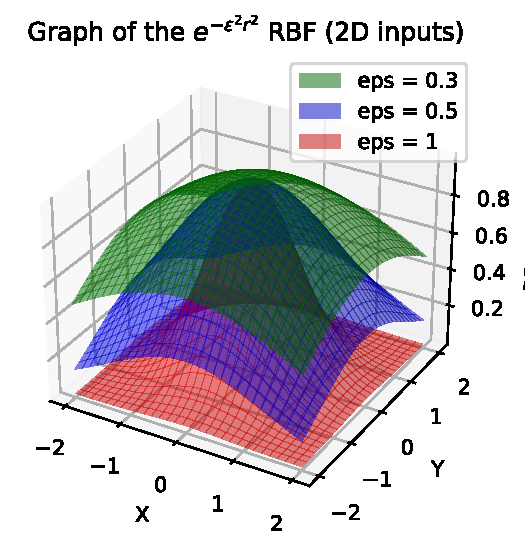
\includegraphics[width=.5\textwidth, clip=true, trim={0 0 .1cm 0}]{imagenes/rbf_discussion/negative-exp-rbf.pdf}}
  \caption{Representation of the radial basis function $e^{-\varepsilon^2 r^2}$. Note that a smaller value of $\varepsilon$ translates into a progressively flatter shape, whereas a larger value of $\varepsilon$ causes the function to feature a more stark cusp.}
  \label{fig:negative-exp-rbf}
\end{figure}

As the previous results show, one needs a firm grasp on Fourier transforms as well as
measure theory to reliably make use of these results and ultimately showing that
the Gaussian function is strictly positive definite. Because of this very reason, we turn
to the last set of (arguably more manageable) theoretical results.

% \subsection*{Characterizations in terms of completely monotone functions}

\begin{definition}
  A function $\varphi : [0, \infty) \rightarrow \mathbb{R}, \varphi \in C [0,
    \infty) \cap C^{\infty} (0, \infty)$ such that
  \[ (- 1)^{l} \varphi^{(l)} (r) \geq 0, \quad r > 0,
    l= 0, 1, 2, \ldots, \]
  is said to be {\tmstrong{completely monotone}} on $[0, \infty)$.
\end{definition}

\begin{theorem}
  \label{thm-completely-monotone-iff-positive-definite-radial}A function
  $\varphi : [0, \infty) \rightarrow \mathbb{R}$ is completely monotone on
  $[0, \infty)$ if and only if $\phi (\cdot) = \varphi (\| \cdot \|^2)$ is
  positive definite and radial on $\mathbb{R}^d$ for all $d$.
\end{theorem}

Note that Theorem \ref{thm-completely-monotone-iff-positive-definite-radial}
imposes a relation between functions $\phi$ and $\varphi$ different to that of
Definition \ref{radialfunctions}. Much like the work we did on Theorem
\ref{tm-bochner}, we will only prove the direction that yields the
positive-definiteness and ``radiality'' on $\mathbb{R}^d$ for all $d$. To this
end, we shall use the following Theorem:

\begin{theorem}
  {\tmstrong{(Hausdorff-Bernstein-Widder)}}\label{thm-hausdorff-bernstein-widder}
  A function $\varphi : [0, \infty) \rightarrow \mathbb{R}$ is completely
  monotone on $[0, \infty)$ if and only if it is the Laplace transform of a
  finite  Borel measure $\mu$ on $[0, \infty)$, that is, if
  \begin{equation}
    \varphi (r) = \int_0^{\infty} e^{- r t} d \mu (t) .
    \label{phi-thm-hausdorff}
  \end{equation}
\end{theorem}

\begin{proof}
  {\tmstrong{(Theorem
      \ref{thm-completely-monotone-iff-positive-definite-radial})}} Applying
  Theorem \ref{thm-hausdorff-bernstein-widder}, we can express $\varphi$ like
  in \eqref{phi-thm-hausdorff}, for a finite Borel measure $\mu$,
  or equivalently in terms of $\| \tmmathbf{x} \|^2$ by noting that $\phi
    (\tmmathbf{x}) = \varphi (\| \tmmathbf{x} \|^2)$. To conclude the positive
  definiteness of $\phi$, we simply check the definition and apply the
  linearity of the integral:
  \begin{equation}\label{eqn-linearity-of-integral}
    \sum_{j = 1}^N \sum_{k = 1}^N c_j c_k \phi (\tmmathbf{x}_j
    -\tmmathbf{x}_k) = \int_0^{\infty} \sum_{j = 1}^N \sum_{k = 1}^N c_j c_k
    e^{- t \| \tmmathbf{x}_j -\tmmathbf{x}_k \|^2} d \mu (t) .
  \end{equation}

  Noting that we integrate on $t \geq 0$, it follows that the quadratic form of
  the integrand involves Gaussian functions, which were shown in Example
  \ref{ex-gaussian-strictly-positive-definite} to be strictly positive
  definite. Consequently, the quadratic form is non-negative, which ultimately
  implies the positive definiteness of $\varphi$.
\end{proof}

\begin{theorem}
  If $\varphi$ is completely monotone but not constant on $[0,\infty)$,
  then the function ${\tmmathbf{x}} \mapsto \varphi(||\tmmathbf{x}||^2)$ is a radial,
  strictly positive definite function on any inner-product space.

  Thus, for any $n$ distinct points
  $\{\tmmathbf{x}_1,\tmmathbf{x}_2,...,\tmmathbf{x}_n\}$
  in such a space, the matrix
  $A_{i,j}=\varphi(||\tmmathbf{x}_i-\tmmathbf{x}_j||)$ is positive definite
  (and therefore nonsingular).
\end{theorem}

\begin{proof}
  Because $\varphi$ is completely monotone, Theorem
  \ref{thm-hausdorff-bernstein-widder} implies that there is a bounded Borel
  measure $\mu$ on $[0, \infty)$ for which \eqref{phi-thm-hausdorff} holds.
  Moreover, $\varphi$ is assumed not to be constant, which implies that $\mu (0,
    \infty) > 0$ and ultimately that $d \mu$ is not concentrated at $0$. Now,
  taking $A_{i, j} = \varphi (\| \tmmathbf{x}_i -\tmmathbf{x}_j \|^2)$ and any
  $c = (c_1, c_2, \ldots, c_n) \neq 0$, we again come upon
  \eqref{eqn-linearity-of-integral}. Recalling that the integrand is positive
  and that the measure is not concentrated at $0$, the result follows.
\end{proof}

In the following, we turn to formulating Problem \ref{interpolationproblemstatement}
with the definitions devised in Section \ref{sec-neural-networks}. Furthermore,
we shall explicitly propose examples to move the discussion forward and identify
concerns on the computational side of the Problem.

\section{Putting it all together: RBF-based neural networks}

The radial basis function method for interpolating a function can then be
proposed and solved by means of a neural network. One of the first works at
this respect was the one carried out by Broomhead and Lowe in 1988
  {\cite{broomhead1988multivariable}}, where they expressed that the linear
dependence of the weights in the radial basis function expansion would allow
for a globally optimum least-squares interpolation of an arbitrary function.

To solve this problem, the multi-layer perceptron \eqref{perceptronRule}
(actually, a three-layer perceptron) was seen to fit the radial basis function
expansion \eqref{eqn-p-is-a-linear-combination-of-rbfs}. Indeed, suppose we want
to interpolate specific realizations of a map $f : \mathbb{R}^d \rightarrow
  \mathbb{R}$ with an RBF expansion of $N$ centers. In such case, multi-layer
perceptron theory allows one to define a function of the form
\[ \begin{array}{cccc}
    \mathcal{N}^3 : & \mathbb{R}^N & \rightarrow & \mathbb{R}                             \\
                    & \tmmathbf{x} & \mapsto     & \sigma_3 (\tmmathbf{W}^3 \mathcal{N}^2
    (\tmmathbf{x}) +\tmmathbf{b}^3)
  \end{array}, \]
where $\tmmathbf{W}^3 \in \mathbb{R}^{1 \times N}$ corresponds to our linear
coefficients $\lambda_1, \lambda_2, \ldots, \lambda_N$, $\tmmathbf{b}^3 \equiv
  \tmmathbf{0}$ and $\sigma_3$ denotes the entry-wise identity operator. By the
same token, we define
\[ \begin{array}{cccc}
    \mathcal{N}^2 : & \mathbb{R}^d & \rightarrow & \mathbb{R}^N                           \\
                    & \tmmathbf{x} & \mapsto     & \sigma_2 (\tmmathbf{W}^2 \mathcal{N}^1
    (\tmmathbf{x}) +\tmmathbf{b}^2)
  \end{array}, \]
where $\tmmathbf{W}^2 \in \mathbb{R}^{N \times d}$ is the identity operator,
$\tmmathbf{b}^2 \equiv \tmmathbf{0}$ and
\[ \sigma_2 (\tmmathbf{x}) = \left(\begin{array}{cccc}
    \varphi (\| \tmmathbf{x}-\tmmathbf{x}_1 \|) & \varphi (\|
    \tmmathbf{x}-\tmmathbf{x}_2 \|)             & \ldots      & \varphi (\|
    \tmmathbf{x}-\tmmathbf{x}_N \|)
  \end{array}\right)^{\top} \]
is the vector whose entries are the application of a certain RBF $\varphi$ to the input
$\tmmathbf{x}$ up to each of our $N$ centers. Consequently, the radial basis
function expansion may be expressed by means of Figure \ref{fig-rbf-drawing}.
\begin{figure}[ht]
  % \frame
  {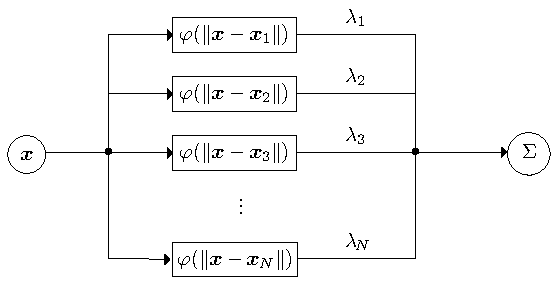
\includegraphics[width=.7\textwidth]{imagenes/rbf_discussion/rbf-nn-graph.pdf}}
  \caption{Depiction of a three-layer perceptron for RBF expansion. The
    initial layer is the input layer, the hidden layer denotes the application
    of the RBF function up to the $N$ centers (the previously-defined operator
    $\sigma_2$), and the final layer denotes their sum up to the coefficients
    $\lambda_1, \lambda_2, \ldots, \lambda_N$ (the previously-defined
    $\tmmathbf{W}^3 \in \mathbb{R}^{1 \times N}$).
    \label{fig-rbf-drawing}}
\end{figure}

So far the discussion has been devoted to tie the apparent distances between
the RBF expansion method with the multi-layer perceptron, to describe the
former in terms of the latter in order to apply well-known machine learning
methods to solve problems with RBFs. Unlike ``traditional'' multi-layer
perceptrons, whose leading idea is often the usage of nested affine
transformations and activation functions to try and solve complex problems
(with the usage of often complex architectures), radial basis function
expansions yield pithy mathematical forms to solve problems that would require
more than one affine transformation if we were to use this ``traditional''
multi-layer perceptron.

Such is the case of the \tmverbatim{xor} operator (``exclusive or''), a
binary operator that obeys the rule expressed in the left-hand side of Table
\ref{table-xor-distances}:

% \begin{table}[h]
%   \begin{tabular}{ll}
%     {\center{\begin{tabular}{|c|c|c|}
%       \hline
%       \tmverbatim{A} & \tmverbatim{B} & \tmverbatim{xor(A,B)}\\
%       \hline
%       0 & 0 & 0\\
%       \hline
%       0 & 1 & 1\\
%       \hline
%       1 & 0 & 1\\
%       \hline
%       1 & 1 & 0\\
%       \hline
%     \end{tabular}}} &
%     \frame
%     {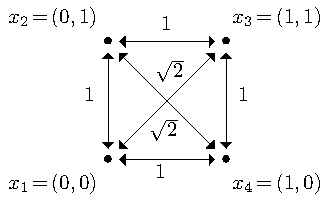
\includegraphics[width=.45\textwidth]{imagenes/rbf_discussion/drawing-xor.pdf}}
%   \end{tabular}
%   \caption{On the left-hand side, the explicit mapping of the \tmverbatim{xor}
%   function for any binary input. On the right-hand side, the localization of
%   the 2D inputs in a plane alongside their pairwise Euclidean distances.
%   \label{table-xor-distances}}
% \end{table}

\begin{table}[h]
  \begin{tabular}{ll}
    \frame
    {\begin{tabular}{|c|c|c|}
         \hline
         \tmverbatim{A} & \tmverbatim{B} & \tmverbatim{xor(A, B)} \\
         \hline
         0              & 0              & 0                      \\
         \hline
         0              & 1              & 1                      \\
         \hline
         1              & 0              & 1                      \\
         \hline
         1              & 1              & 0                      \\
         \hline
       \end{tabular}} &
    {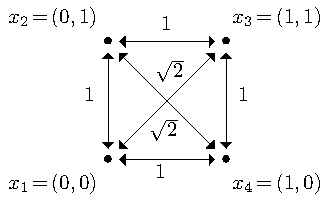
\includegraphics[width=.41\textwidth]{imagenes/rbf_discussion/drawing-xor.pdf}}
  \end{tabular}
  \caption{On the left-hand side, the explicit mapping of the \tmverbatim{xor}
    function for any binary input. On the right-hand side, the localization of
    the 2D inputs in a plane alongside their pairwise Euclidean distances.
  }
  \label{table-xor-distances}
\end{table}

Notice that the two pairs of points for which we wish to produce the same
output always maximize their distance (see right-hand side of Table
\ref{table-xor-distances}). This immediately shows the unfeasibility of using
a single hyperplane as a classifier (i.e., as a function returning either 0 or
1 for our inputs). In other words: we cannot solve this problem by means of a
single affine transformation.

However, we can solve this problem in terms of an RBF expansion, that is, in
terms of a neural network with a single hidden layer. To this end, note that
we have defined the \tmverbatim{xor} operator by extension: there are exactly
four bi-dimensional possible inputs. It is in those inputs where our centers will be located.
Considering so far an arbitrary radial basis function $\varphi (\| \cdot \|)$
and operating under the Euclidean norm, we wish to find a function $\sum_{i =
    1}^4 \lambda_i \varphi (\| \tmmathbf{x}-\tmmathbf{x}_j \|_2)$, where
$\tmmathbf{x}_1, \tmmathbf{x}_2, \tmmathbf{x}_3, \tmmathbf{x}_4$ are distanced as in the
right-hand side of Table \ref{table-xor-distances}. Consequently,
\eqref{eqn-linear-system-equations-rbf} is now expressed as
\begin{equation}
  \left(\begin{array}{cccc}
      \varphi (0)                       & \varphi (1)                     & \varphi \left( \sqrt{2} \right) & \varphi
      (1)                                                                                                                             \\
      \varphi (1)                       & \varphi (0)                     & \varphi (1)                     & \varphi \left( \sqrt{2}
      \right)                                                                                                                         \\
      \varphi \left( \sqrt[]{2} \right) & \varphi (1)                     & \varphi (0)                     & \varphi
      (1)                                                                                                                             \\
      \varphi (1)                       & \varphi \left( \sqrt{2} \right) & \varphi (1)                     & \varphi (0)
    \end{array}\right) \left(\begin{array}{c}
      \lambda_1 \\
      \lambda_2 \\
      \lambda_3 \\
      \lambda_4
    \end{array}\right) = \left(\begin{array}{c}
      0 \\
      1 \\
      0 \\
      1
    \end{array}\right) .\label{interpolationconditionxor}
\end{equation}

Calling $A$ the real symmetric matrix on the left-hand side of the equation,
and under suitable radial basis functions such that $A$ is full rank, we have
$A = V \mu V^{\top}$ with $V$ an orthogonal matrix (which is such that $V^{\top} =
  V^{- 1}$) and $\mu$ a diagonal matrix with nonzero entries. Therefore, we can
compute the inverse of $A$ by means of the matrix product
\begin{equation}
  A^{- 1} = V \mu^{- 1} V^{\top} . \label{eqn-a-inverse-eigenvectors}
\end{equation}
Actually, we can find an analytic expression\footnote{Refer to Appendix A of
    {\cite{broomhead1988multivariable}} (Table 2 and equations A.4, A.5) for precise computation details.} for $V$
and $\mu$, which ultimately allows us to solve for $A$. It is
\[ V = \frac{1}{2} \left(\begin{array}{rrrr}
      1 & 1   & \sqrt{2}   & 0          \\
      1 & - 1 & 0          & - \sqrt{2} \\
      1 & 1   & - \sqrt{2} & 0          \\
      1 & - 1 & 0          & - \sqrt{2}
    \end{array}\right), \text{ alongside } \]
\begin{equation}
  \mu = \left(\begin{array}{cccc}
      \mu_1 & 0     & 0     & 0     \\
      0     & \mu_2 & 0     & 0     \\
      0     & 0     & \mu_3 & 0     \\
      0     & 0     & 0     & \mu_3
    \end{array}\right), \text{ for } \left\{\begin{array}{l}
    \mu_1 = \varphi (0) + 2 \varphi (1) + \varphi \left( \sqrt{2} \right) \\
    \mu_2 = \varphi (0) - 2 \varphi (1) + \varphi \left( \sqrt{2} \right) \\
    \mu_3 = \varphi (0) - \varphi \left( \sqrt{2} \right)
  \end{array}\right. . \label{eqn-mu-analytic-eigenvector}
\end{equation}
Because $V$ is an orthogonal matrix, the existence of $A^{- 1}$ is tied to the
existence of $\mu^{- 1}$, as per \eqref{eqn-a-inverse-eigenvectors}. This is
equivalent to say that we need $\mu_1, \mu_2, \mu_3$ to be nonzero, which
entirely depends on the choice of $\varphi$: reasoning on
\eqref{eqn-mu-analytic-eigenvector}, we note that $\mu_3 = 0 \Leftrightarrow
  \varphi (0) = \varphi \left( \sqrt{2} \right)$. Likewise, $\mu_1 = 0
  \Leftrightarrow \varphi (1) = - \frac{\varphi (0) + \varphi \left( \sqrt{2}
    \right)}{2}$ and $\mu_2 = 0 \Leftrightarrow \varphi (1) = \frac{\varphi (0) +
    \varphi \left( \sqrt{2} \right)}{2}$. Provided we have carefully chosen the
RBFs to avoid null eigenvalues, we may explicitly compute the parameters
vector $\underline{\lambda}$ as in \eqref{matrixexpression-interpolationprob}
for problem \eqref{interpolationconditionxor}. To this end, let $f = (0, 1, 0,
  1)^{\top}$ denote the right-hand side column vector (to be expressed in terms of the orthogonal vectors conforming $V$), whereupon
\[ \underline{\lambda} = A^{- 1} f = V \mu^{- 1} V^{\top} f = V \mu^{- 1}
  V^{\top} \frac{1}{2} \left[ \left(\begin{array}{c}
      1 \\
      1 \\
      1 \\
      1
    \end{array}\right) - \left(\begin{array}{r}
      1   \\
      - 1 \\
      1   \\
      - 1
    \end{array}\right) \right] = V \mu^{- 1} \left[ \left(\begin{array}{c}
      1 \\
      0 \\
      0 \\
      0
    \end{array}\right) - \left(\begin{array}{c}
      0 \\
      1 \\
      0 \\
      0
    \end{array}\right) \right] = \]
\[ = V \left(\begin{array}{r}
      \mu_1^{- 1}   \\
      - \mu_2^{- 1} \\
      0             \\
      0
    \end{array}\right) = \frac{1}{2} \left(\begin{array}{c}
      \mu_1^{- 1} - \mu_2^{- 1} \\
      \mu_1^{- 1} + \mu_2^{- 1} \\
      \mu_1^{- 1} - \mu_2^{- 1} \\
      \mu_1^{- 1} + \mu_2^{- 1}
    \end{array}\right) \Rightarrow \underline{\lambda} = \left(\begin{array}{c}
      \lambda_1 \\
      \lambda_2 \\
      \lambda_3 \\
      \lambda_4
    \end{array}\right) = \left(\begin{array}{c}
      \lambda_1 \\
      \lambda_2 \\
      \lambda_1 \\
      \lambda_2
    \end{array}\right) . \]
Substituting now \eqref{eqn-mu-analytic-eigenvector} in this last equation and expanding, we
conclude that \begin{equation}
  \lambda_1 = - \frac{2 \varphi (1)}{\left( \varphi (0) + \varphi
    \left( \sqrt{2} \right) \right)^2 - 4 \varphi (1)^2}, \text{ and } \lambda_2 =
  \frac{\varphi (0) + \varphi \left( \sqrt{2} \right)}{\left( \varphi (0) +
    \varphi \left( \sqrt{2} \right) \right)^2 - 4 \varphi (1)^2}.
  \label{eqn-lda1-lda2}
\end{equation}

\begin{figure}[ht]
  \centering
  \begin{tabular}{ll}
    % \frame
    {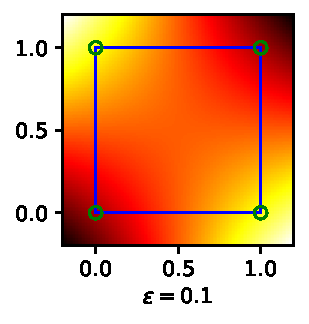
\includegraphics[width=.33\textwidth]{imagenes/xor/xor0.1.pdf}} & 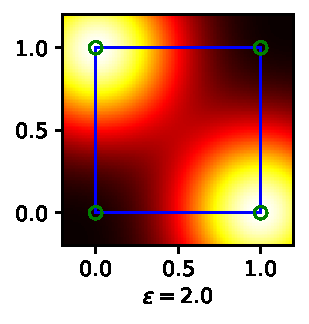
\includegraphics[width=.33\textwidth]{imagenes/xor/xor2.0.pdf} \\
    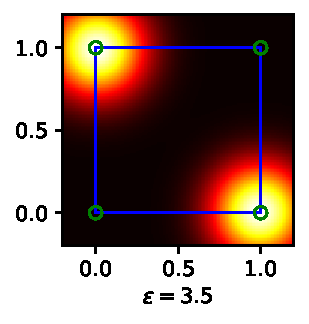
\includegraphics[width=.33\textwidth]{imagenes/xor/xor3.5.pdf}   & 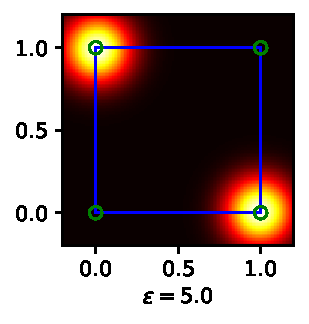
\includegraphics[width=.33\textwidth]{imagenes/xor/xor5.0.pdf}
  \end{tabular}
  \begin{tabular}{r}
    % \frame
    {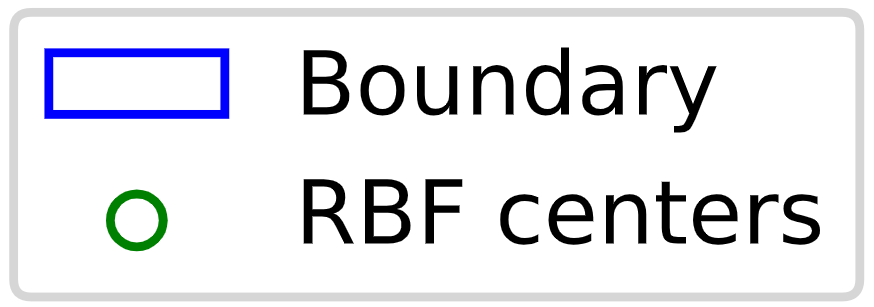
\includegraphics[width=.24\textwidth, trim={0 -2cm 0 0}, clip=true]{imagenes/xor/Legend.png}}
    \\
    {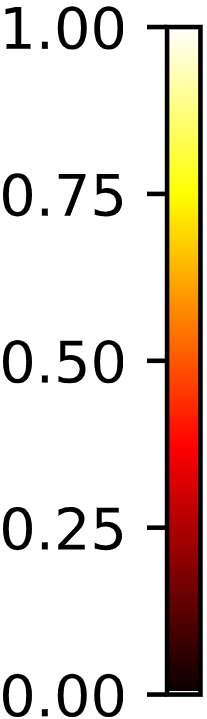
\includegraphics[height=.4\textwidth]{imagenes/xor/Colorbar.png}}
  \end{tabular}
  \caption{Contour of the \texttt{xor} binary operator with a Gaussian RBF expansion for different values of the shape parameter $\varepsilon$. In coherence with Figure \ref{fig:negative-exp-rbf}, larger values of $\varepsilon$ translate into starker cusps (see figures for $\varepsilon=3.5,5.0$).}
  \label{fig:xor}
\end{figure}

We refer to Figure \ref{fig:xor} for a comparison on the interpolation of the
four values provided for the \tmverbatim{xor} operator with a Gaussian RBF
under different values of the shape parameter $\varepsilon$. If we were
instead dealing in a fuzzy logic\footnote{See {\cite{zadeh1988fuzzy}} or
    {\cite{russell2005ai}} for starting pointers.} setting, whereby the truth
value of a statement would now take values in $[0, 1]$, the shape parameter
would be instrumental in determining an appropriate set of such intermediate
truth values. One must bear in mind that this example, where we have been able
to determine an explicit form of $\underline{\lambda}$ without explicitly
inverting matrix $A$, is not going to happen in general.

\begin{definition}
  Let $A \in \mathbb{R}^{n \times n}$. The number
  \[ \kappa_{\| \cdot \|} (A) = \| A^{- 1} \| \cdot \| A \| \]
  is said to be the {\tmstrong{condition number}} for inverting $A$ under the
  norm $\| \cdot \|$.
\end{definition}

Provided we wish to solve a system of the form $A \underline{\lambda} = f$,
with $A, \underline{\lambda} \text{ and } f$ as in
\eqref{eqn-linear-system-equations-rbf}, our previous discussion shows that there
are two key components that determine the condition number of the inversion of
$A$: the particular {\tmstrong{choice of RBFs}} and the {\tmstrong{location of
      the centers}}. We address the former component for now.

To this end, we refer to the left-hand side of Figure
\ref{fig:xor-coefficients-conditioning} and note that the condition number of
the inverse increases linearly as $\varepsilon$ ranges (roughly) from $1$ to
$10^{- 1}$. Further reducing the value of the shape parameter cues in an
ill-conditioned problem, for which the condition number of the matrix
notoriously oscillates. This ultimately causes the coefficients of the RBF
expansion to increase in orders of magnitude {\cite{fornberg2015primer}}, as
the right-hand side of Figure \ref{fig:xor-coefficients-conditioning} shows.
Consequently, if we are to optimize the parameters of a neural network
implemented as in \ref{fig-rbf-drawing} (which is a direct implementation of
the RBF expansion), the search for suitable coefficients to solve the
interpolation problem of the \tmverbatim{xor} operator would see us choosing
some shape parameter $\varepsilon > 1$.

This observation leads us now into the search for other RBFs, with (maybe)
more suitable condition numbers for the inversion of the matrix of the
scattered data interpolation problem.

\begin{figure}[ht]
  \centering
  % \frame
  {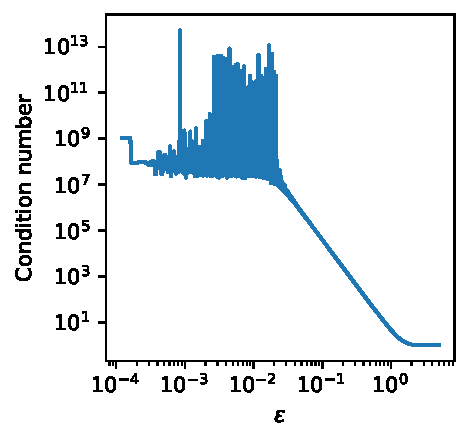
\includegraphics[width=.45\textwidth]{imagenes/xor/xor_conditioning_graph.pdf}}
  {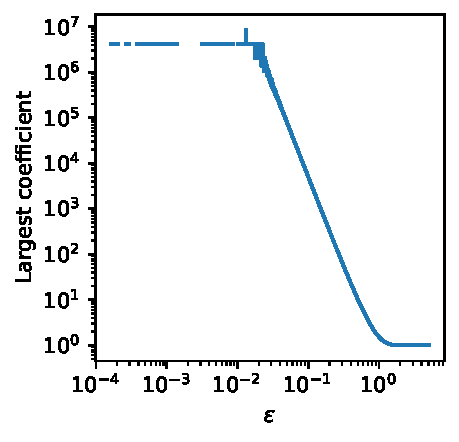
\includegraphics[width=.45\textwidth]{imagenes/xor/xor_largest_coef_graph.pdf}}
  \caption{Left-hand side: the condition number of the inversion of matrix $A$ of the \texttt{xor} binary operator interpolation problem. Right-hand side: order of magnitude of the largest (in absolute value) coefficient of the RBF expansion. Note that the ``empty'' values in the right-hand side figure are due to the numerical computation of the coefficients $\lambda_1, \lambda_2$ in \eqref{eqn-lda1-lda2} returning a value too large for the system's floating point system, which then defaults to infinity.}
  \label{fig:xor-coefficients-conditioning}
\end{figure}

To this end, following Micchelli's discussion \cite{micchelli1984interpolation} we generalize the radial basis function expansion \eqref{eqn-p-is-a-linear-combination-of-rbfs} into the form
\begin{equation}
  \mathcal{P} (\tmmathbf{x}) = \sum_{i = 1}^N \lambda_i \phi_j (\tmmathbf{x})
  + \sum_{i = 1}^m \mu_i p_i (\tmmathbf{x}), \quad m \leq n,
  \label{eqn-rbf-poly}
\end{equation}
where each $\phi_j : \mathbb{R}^d \rightarrow \mathbb{R}$ is such that
$\phi_j (\tmmathbf{x}) = \varphi (\| \tmmathbf{x}-\tmmathbf{x}_j \|)$ for a
fixed $\tmmathbf{x}_j \in \mathbb{R}^d$ and $\varphi : [0, \infty) \rightarrow
  \mathbb{R}$ is a continuous function. Furthermore, we prescribe that
$\tmop{span} \{ p_1, p_2, \ldots, p_m \}$ should be equal to $\mathbb{P}_{k -
    1} (\mathbb{R}^d)$, the space of polynomials of total degree $\leq k - 1$.



\begin{definition}\label{def-rbf-poly}
  Let $\varphi : [0, \infty) \rightarrow \mathbb{R}$ be a continuous function,
  $\{ \tmmathbf{x}_j \}_{j = 1}^N \subset \mathbb{R}^d$ a set of distinct
  points and $(\lambda_1, \lambda_2, \ldots, \lambda_N) \in \mathbb{R}^N$ such
  that
  \begin{equation}
    \sum_{i = 1}^N \lambda_i p (\tmmathbf{x}_i) = 0
    \label{constraint-rbf-polynomial}
  \end{equation}
  for all $p \in \mathbb{P}_{k - 1} (\mathbb{R}^d)$. If the quadratic form
  \[ \sum_{i = 1}^N \sum_{j = 1}^N \lambda_i \lambda_j \varphi (\|
    \tmmathbf{x}_i -\tmmathbf{x}_j \|) \]
  is non-negative (resp., positive), then $\varphi$ is said to be
    {\tmstrong{conditionally positive}} (resp. {\tmstrong{conditionally strictly
        positive}}) {\tmstrong{definite of order $k$}} on $\mathbb{R}^d$.
\end{definition}

% We now extend Theorem
% \ref{thm-completely-monotone-iff-positive-definite-radial} to functions of the
% form \eqref{eqn-rbf-poly}.

\begin{theorem}
  If $\varphi \in C [0, \infty)$ and $(- 1)^k \varphi^k(r)$ is
  completely monotone on $(0, \infty)$, then $\varphi$ is conditionally
  positive of order $k$.
\end{theorem}

For the sake of clarity, \eqref{constraint-rbf-polynomial} can be formulated
as
\[ \sum_{i = 1}^N \lambda_i = \sum_{i = 1}^N \lambda_i x_i = \sum_{i = 1}^N \lambda_i
  x^2_i = \cdots = \sum_{i = 1}^N \lambda_i x^m_i = 0, \]
which allows one to consider the system
\[ \left[\begin{array}{ccc|ccccc}
                                  &        &                             & {\color[HTML]{008000}1} & {\color[HTML]{008000}x_1} &
      {\color[HTML]{008000}x_1^2} & \ldots & {\color[HTML]{008000}x_1^m}                                                                            \\
                                  & A      &                             & \vdots                  & \vdots                    & \vdots &  & \vdots \\
                                  &        &                             & {\color[HTML]{008000}1} & {\color[HTML]{008000}x_N} &
      {\color[HTML]{008000}x_N^2} & \ldots & {\color[HTML]{008000}x_N^m}                                                                            \\ \hline
      1                           & \ldots & 1                           &                         &                           &        &  &        \\
      x_1                         & \ldots & x_N                         &                         &                           &        &  &        \\
      x_1^2                       & \ldots & x_N^2                       &                         &                           & 0      &  &        \\
      \vdots                      &        & \vdots                      &                         &                           &        &  &        \\
      x_1^m                       & \ldots & x_N^m                       &                         &                           &        &  &
    \end{array}\right] \left[\begin{array}{c}
      \lambda_1 \\
      \vdots    \\
      \lambda_N \\
      \hline
      \mu_1     \\
      \mu_2     \\
      \mu_3     \\
      \vdots    \\
      \mu_m
    \end{array}\right] = \left[\begin{array}{c}
      f_1    \\
      \vdots \\
      f_N    \\
      \hline
      0      \\
      0      \\
      0      \\
      \vdots \\
      0
    \end{array}\right] \]
expressed in the more compact notation
\begin{equation}
  \left[\begin{array}{cc}
      A        & P            \\
      P^{\top} & \tmmathbf{0}
    \end{array}\right] \left[\begin{array}{c}
      \underline{\lambda} \\
      \underline{\mu}
    \end{array}\right] = \left[\begin{array}{c}
      \underline{f} \\
      \tmmathbf{0}
    \end{array}\right]. \label{eqn-augmented-rbf-poly-system}
\end{equation}

The submatrix with entries in green is of dimensions $n \times (m + 1)$. Therefore, the
resulting matrix is square and of size $(m + n + 1) \times (m + n + 1)$.

We will return to these functions in the coming discussions. For now, we turn to another set of results, which will allow us to present the \textbf{multiquadric} radial basis function. To do so, we follow the discussion presented in \cite{sarra2009multiquadric}:

\begin{theorem}
  Assume $\varphi'(r)$ is completely monotone and not constant on
  $(0, \infty)$, $\varphi \in C [0, \infty)$ and $\varphi (r) > 0$ for $r >
    0$. Denote by $A$ the matrix in \eqref{eqn-linear-system-equations-rbf}. Then,
  for any distinct $\{ \tmmathbf{x}_j \}_{j = 1}^N \subset \mathbb{R}^d$
  \[ (- 1)^{N - 1} \det A > 0, \]
  which implies the invertibility of $A$.
  \label{thm-A-invertible}
\end{theorem}

\begin{example}
  Under these few new results, and letting $m = 0$ in \eqref{eqn-rbf-poly},
  one can already consider the multiquadric (MQ) radial basis function,
  $\varphi (r) = \sqrt{1 + \varepsilon^2 r} > 0$. Note that
  \[ \begin{array}{ccl}
      \varphi' (r)      & = & \frac{\varepsilon^2}{2} (\varepsilon^2 r + 1)^{- 1 /
      2}                                                                           \\
      \varphi'' (r)     & = & - \frac{\varepsilon^4}{4} (\varepsilon^2 r + 1)^{-
      3 / 2}                                                                       \\
      \varphi''' (r)    & = & \frac{3 \varepsilon^6}{8} (\varepsilon^2 r + 1)^{-
      5 / 2}                                                                       \\
      \varphi^{(4)} (r) & = & - \frac{15 \varepsilon^8}{16} (\varepsilon^2 r
      + 1)^{- 7 / 2}
    \end{array} . \]
  We observe that $(- 1)^l \varphi^{(l)} (r) \leq 0$ for all $r \geq 0$ and $l
    = 0, 1, 2, \ldots$, due to the changes in sign introduced by the derivative
  with respect to $r$ of $(\varepsilon^2 r + 1)^{- \beta}, \beta > 0$. It
  follows that $\varphi' (r)$ is completely monotone. It is also immediate to
  see that $\varphi' (r) > 0$ is not constant. Finally, the largest possible
  domain of $\varphi$ is $r \geq - 1 / \varepsilon^2$, for which it also is
  continuous. Since we assume $r \geq 0$, Theorem \ref{thm-A-invertible}
  guarantees the invertibility of the corresponding the interpolation matrix for
  any scattered data interpolation problem.
\end{example}

It is common to consider also this multiquadric RBF under the formulation
$\varphi (r) = \sqrt{1 + \varepsilon^2 r^2}$. We depict this alternative in
Figure \ref{fig:mq-rbf} under different values of the shape parameter
$\varepsilon$.

\begin{figure}[ht]
  \centering
  % \frame
  {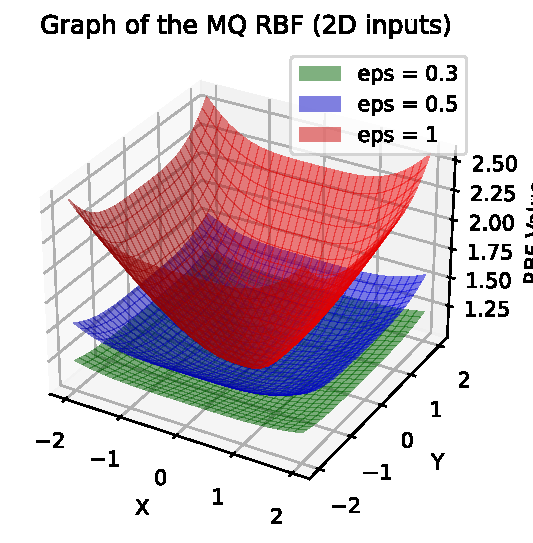
\includegraphics[width=.5\textwidth, clip=true, trim={0 0 .17cm 0}]{imagenes/rbf_discussion/mq-rbf.pdf}}
  \caption{Representation of the multiquadric radial basis function $\sqrt{1+\varepsilon^2 r^2}$. Much like in the case \ref{fig:negative-exp-rbf}, that a smaller value of $\varepsilon$ translates into a progressively flatter shape, whereas a larger value of $\varepsilon$ causes the function to feature a more stark cusp.}
  \label{fig:mq-rbf}
\end{figure}

\subsection*{Some ``pathological'' examples}

As pointed out in Theorem \ref{thm-haar-spaces-polynomials}, pre-fixed
generalized polynomials are not apt for interpolation problems of
dimension larger than one. Polynomials\footnote{We are not referring to generalized polynomials in this stretch of the discussion.}, which
have not been discussed up until now, can still be used for one-dimensional
problems. This is the motivation behind the next case study, where we consider
$x \mapsto \frac{1}{1 + 25 x^2}$, referred to as the {\tmstrong{Runge
      function}}. Figure \ref{fig:runge-polynomial-interpolation} depicts the
interpolation of this function on a progressively more populated equispaced
grid, which increases the degree of the interpolating polynomial under consideration\footnote{Experiment generated in the context of the \href{https://github.com/heqro/tfm-experiments/blob/main/introductory_notebooks/polynomial_interpolation/runge.ipynb}{polynomial interpolation notebook} featured in the repository.}.

Prior to seeing this depiction, one could mistakenly believe that supplying a larger number of interpolation points would decrease the error in between the interpolation nodes. For this particular function, it can be easily seen such is not the case. For instance, the interpolating polynomial of degree $10$ can be seen to reach large values for inputs close to the boundary of the problem\footnote{On a second (deeper) thought, this phenomenon is not that surprising: if the only information we provide is the value of the function at very specific nodes, we do not necessarily know the value of the interpolator at ``intermediate points''.}. However, the following Theorem states that a suitable polynomial can still be found:

\begin{figure}[ht]
  \centering
  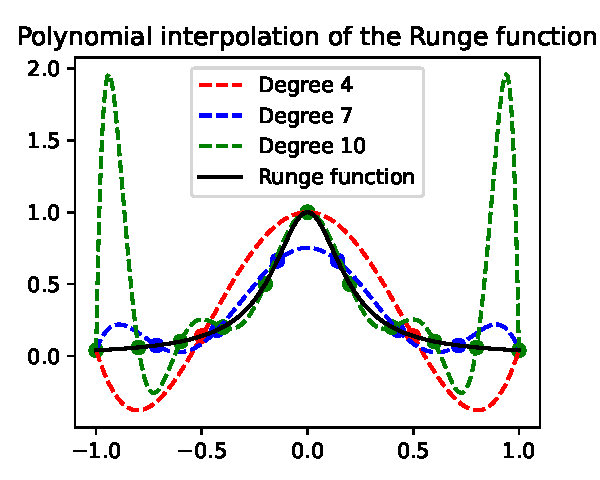
\includegraphics[width=.55\textwidth]{imagenes/polynomial_interpolation/Runge_Polynomial_interpolation.pdf}
  \caption{Polynomial interpolation of the Runge function with $n=5,8,11$ equispaced points. As one can see, larger degrees of the interpolating polynomial do not necessarily imply that the approximation will be close to the actual function between each pair of interpolation nodes.}
  \label{fig:runge-polynomial-interpolation}
\end{figure}

\begin{theorem}
  \label{thm-polynomial-convergence}Let $f$ be a continuous function defined
  on $[a, b]$. For all $\varepsilon > 0$ there corresponds a polynomial $P$
  such that $\| f - P \|_{\infty} < \varepsilon$.
\end{theorem}

A proof of this Theorem is featured in \cite{cheney1966introduction}, where an explicit form of $P$ is given by means of the sequence of
\textbf{Bernstein polynomials}, defined for each $n \in \mathbb{N}$ as
\begin{equation}
  (B_n f) (x) = \sum_{k = 0}^n f \left( \frac{k}{n} \right) \binom{n}{k} x^k
  (1 - x)^{n - k} \label{eqn-bernstein-polynomial},
\end{equation}
for $x \in [0, 1]$. After proposing this polynomial, it is shown that $B_n$ is
a monotone operator. Recall that an operator $L$ is said to be monotone if $f
  \geq g \Rightarrow L f \geq L g$. Assuming that, for any $n\in \mathbb{N}$ the operator $B_n$ is monotone, the following Theorem can be
used:

\begin{theorem}
  \label{thm-monotone-operators}Let $L_n \subset C [a, b]$ be a sequence of
  monotone linear operators. The following conditions are equivalent:
  \begin{enumerate}
    \item $L_n f \rightarrow f$ (uniformly) for all $f \in C [a, b]$.
    \item $L_n f \rightarrow f$ for $f (x) = 1, x, x^2$.
    \item $L_n 1 \rightarrow 1$ and $(L_n \phi_t) (t) \rightarrow 0$ uniformly
          in $t$, where $\phi_t (x) = (t - x)^2$.
  \end{enumerate}

\end{theorem}

\begin{proof}
  ({\tmstrong{Theorem}} \ref{thm-polynomial-convergence}) It suffices to show
  that the second property of Theorem \ref{thm-monotone-operators} holds.
  To this end, note that
  \[ (B_n 1) (x) = \sum_{k = 0}^n \binom{n}{k} x^k (1 - x)^{n - k} = [x + (1 -
        x)]^n = 1^n = 1. \]
  For $f (x) = x$, note that
  \[ (B_n f) (x) = \sum_{k = 0}^n \frac{k}{n} \binom{n}{k} x^k (1 - x)^{n - k}
    = x \sum_{k = 1}^n \binom{n - 1}{k - 1} x^{k - 1} (1 - x)^{n - k} = x
    \sum_{k = 0}^{n - 1} \binom{n - 1}{k} x^k (1 - x)^{n - 1 - k} = \]
  \[ = x (x + (1 - x))^{n - 1} = x. \]
  Finally, for $f (x) = x^2$ we have that
  \[ (B_n f) (x) = \sum_{k = 0}^n \left( \frac{k}{n} \right)^2 \binom{n}{k}
    x^k (1 - x)^{n - k} = \sum_{k = 1}^n \frac{k}{n} \binom{n - 1}{k - 1} x^k
    (1 - x)^{n - k} = \]
  \[ = \frac{n - 1}{n} \sum_{k = 1}^n \frac{k - 1}{n - 1} \binom{n - 1}{k - 1}
    x^k (1 - x)^{n - k} + \frac{1}{n} \sum_{k = 1}^n \binom{n - 1}{k - 1} x^k
    (1 - x)^{n - k} = \frac{n - 1}{n} x^2 + \frac{1}{n} x \xrightarrow[n]{}
    x^2 . \]
  Consequently, $B_n f \rightarrow f$ uniformly for all $f \in C [0, 1]$.
\end{proof}

The left-hand side of Figure \ref{fig:bernstein-runge} shows the absolute error when using Bernstein polynomials to approximate the Runge function\footnote{Experiment generated in the context of the \href{https://github.com/heqro/tfm-experiments/blob/main/introductory_notebooks/bernstein_polynomials/bernstein.ipynb}{Bernstein polynomial interpolation notebook} featured in the repository. We operate with the Runge function, albeit scaled to fit in the $[0,1]$ interval.}. Notice that we indeed have uniform convergence: for increasing values of $n$ as in \eqref{eqn-bernstein-polynomial}, the $L^\infty-$norm with respect to the Runge function decreases.

However, the right-hand side of this same picture allows us to confirm the shortcomings of Bernstein polynomials, which are due to rounding errors. For instance, cancellation occurs for large enough values of $n$ and $k$, which may in turn cause the evaluation of $(1-x)^{n-k}$ to default to $(1-x)$, altering the final result.

\begin{figure}[ht]
  \centering
  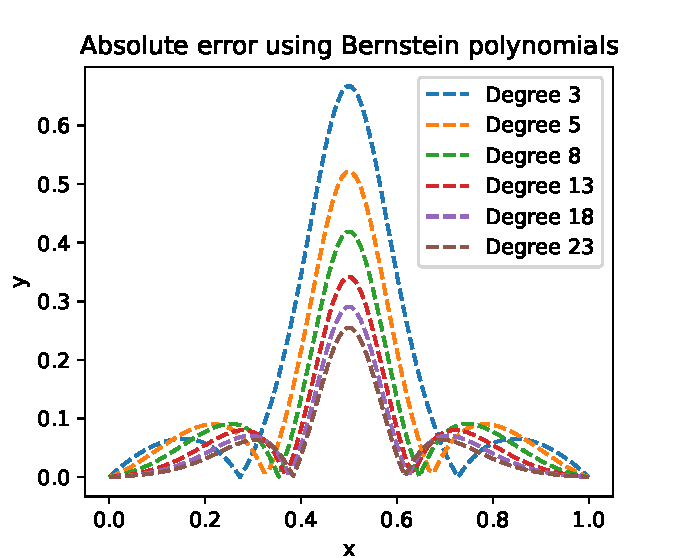
\includegraphics[width=.5\textwidth]{imagenes/bernstein/Bernstein_Polynomials_Runge.pdf}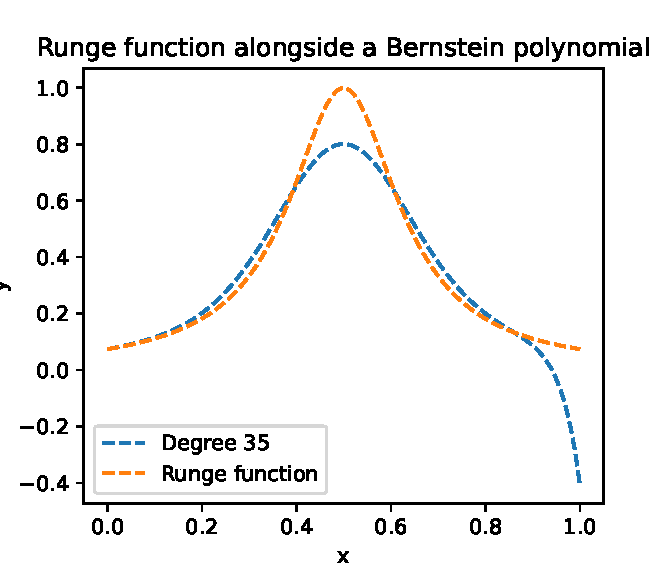
\includegraphics[width=.5\textwidth]{imagenes/bernstein/Bernstein_Polynomials_Runge_D35.pdf}
  \caption{Left-hand side: absolute error when using Bernstein polynomials of progressively higher degrees to approximate the Runge function. Right-hand side: a representation of the Runge function alongside a polynomial of higher degree.}
  \label{fig:bernstein-runge}
\end{figure}

Lastly, dismissing for a moment the computational issues and regarding only the mathematical framework, this polynomial \textit{happens} to be an interpolating polynomial because it can approximate the function to an arbitrary precision, but it requires us to provide an amount of information that is not proper of a scattered data interpolation problem, which ultimately rules out its utility for an interpolation task.

An effective alternative that does not involve Bernstein polynomials comes
from the consideration of a different set of interpolation points, the
so-called {\tmstrong{Chebyshev nodes}}. A set of Chebyshev nodes featuring $n$
points is defined as the family
\begin{equation}
  \left\{ \cos \left( \frac{2 k + 1}{2 n} \cdot \pi \right) \right\}_{k =
  0}^{n - 1} \label{eqn-chebyshev-nodes} \subset (- 1, 1),
\end{equation}
depicted in Figure \ref{fig:chebyshev-nodes}.

\begin{figure}[ht]
  \centering
  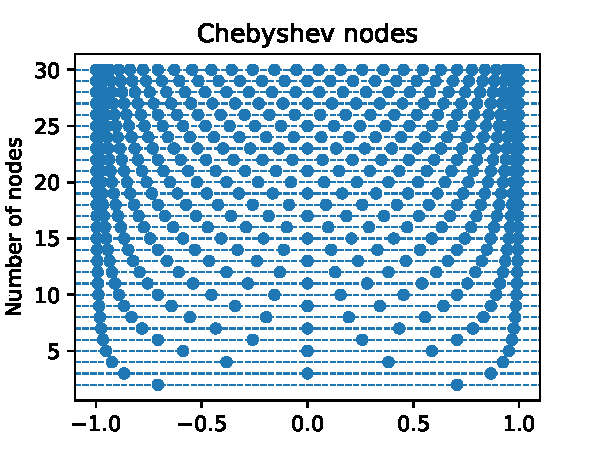
\includegraphics[width=.5\textwidth]{imagenes/polynomial_interpolation/Chebyshev_Nodes.pdf}
  \caption{Distribution of Chebyshev nodes alongside the horizontal axis for an increasing number of nodes.}
  \label{fig:chebyshev-nodes}
\end{figure}



Applying these nodes to the
interpolation of the Runge function\footnote{Experiment generated in the context of the \href{https://github.com/heqro/tfm-experiments/blob/main/introductory_notebooks/polynomial_interpolation/runge_chebyshev.ipynb}{Chebyshev nodes polynomial interpolation notebook} featured in the repository.} (as depicted in Figure
\ref{fig:runge-polynomial-cheb}) shows the effectiveness of the strategy,
whereby we have managed to severely reduce the oscillations between each pair
of interpolation nodes up to the point of guaranteeing a relative error
smaller than $10^{- 1}$ in the case we consider $n = 20$ points.

\begin{figure}[ht]
  \centering
  % \frame
  {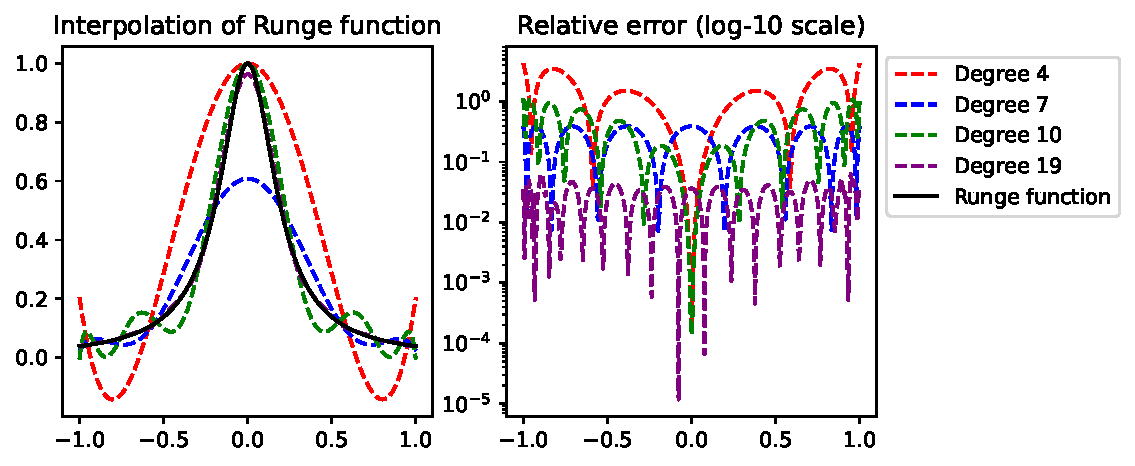
\includegraphics[width=\textwidth]{imagenes/polynomial_interpolation/Runge_Polynomial_Cheb.pdf}}
  \caption{Left-hand side: polynomial interpolation of the Runge function for $n=5, 8, 11, 20$ points distributed as in \eqref{eqn-chebyshev-nodes}. Right-hand side: the corresponding relative error in logarithmic scale.}
  \label{fig:runge-polynomial-cheb}
\end{figure}

As a side note,
it is not strictly necessary to resample the function over the new points of interest. That is, one may re-map the $x-$values of the function to the Chebyshev points while keeping the $y-$values intact and further reducing the oscillations. See for instance \cite{DEMARCHI2021125628} and, most interestingly, their proposed \href{https://github.com/pog87/FakeNodes/blob/master/Runge.ipynb}{associated code sample} for the Runge function.

Gaussian RBFs are able to further reduce this oscillation problem without the need of considering a separate points distribution. Figure \ref{fig:rbf-runge-phenomenon-eps-5-discussion} generated in the context of the linked \href{https://github.com/heqro/tfm-experiments/blob/main/introductory_notebooks/rbf_interpolation/runge_rbf.ipynb}{Gaussian RBF interpolation notebook} depicts that precision up to the first decimal place can be guaranteed, for instance, by considering 9 equispaced centers alongside a suitable shape parameter $\varepsilon=5$.

\begin{figure}[ht]
  \centering
  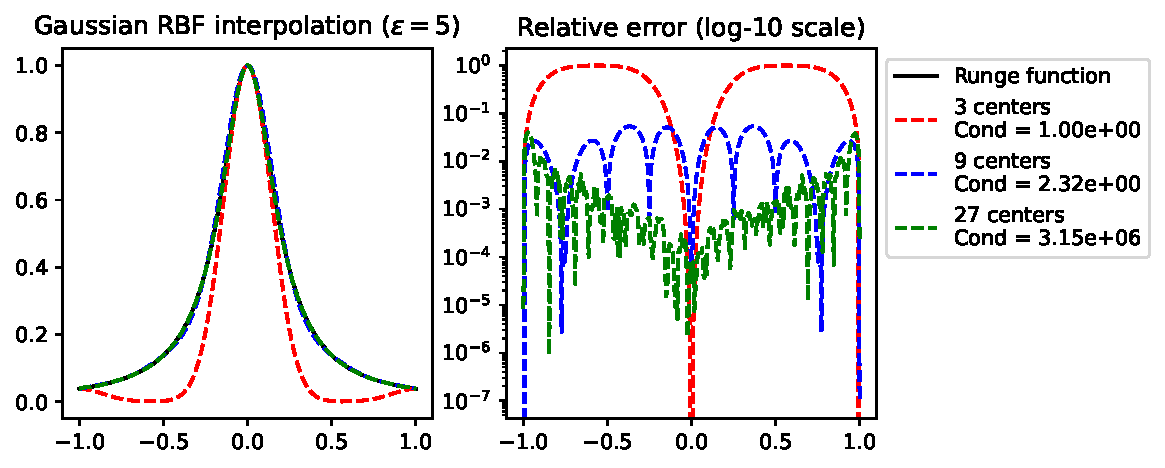
\includegraphics[width=\textwidth]{imagenes/rbf_interpolation/rbf_runge_5.pdf}
  \caption{Left-hand side: Gaussian RBF interpolation of the Runge function for $n=3,9,27$ equispaced points and $\varepsilon=5$. Right-hand side: relative error in logarithmic scale. Furthermore, the legend depicts the condition number of the matrix inversion problem.}
  \label{fig:rbf-runge-phenomenon-eps-5-discussion}
\end{figure}

As previously mentioned, the shape parameter plays a decisive role in the condition number of the matrix.
To avoid explicitly choosing a shape parameter, \textbf{polyharmonic splines} (PHS) are defined by equipping a polynomial of degree larger than the unit to a suitable radial function, usually chosen $r^m,m$ odd, as in \eqref{eqn-rbf-poly}. We refer to Figures \ref{fig:phs-runge-phenomenon-deg-1-discussion} and \ref{fig:phs-runge-phenomenon-deg-3-discussion} for similar charts on the performance of PHS on the Runge function with $r^1$ and $r^3$ respectively\footnote{Images generated in the \href{https://github.com/heqro/tfm-experiments/blob/main/introductory_notebooks/rbf_interpolation/runge_phs.ipynb}{PHS Runge interpolation notebook}.}. Note that the exponent we choose will dictate the behavior of the function between every pair of interpolation nodes. Indeed, $r^1$ dictates that our interpolator will essentially ``join the dots with a straight line'', whereas $r^3$ will instead employ a cubic term.

Even though the latter strategy is preferred for convergence reasons, by a numerical argument one can see why using a large exponent is not always bound to increase our results.

\begin{figure}[ht]
  \centering
  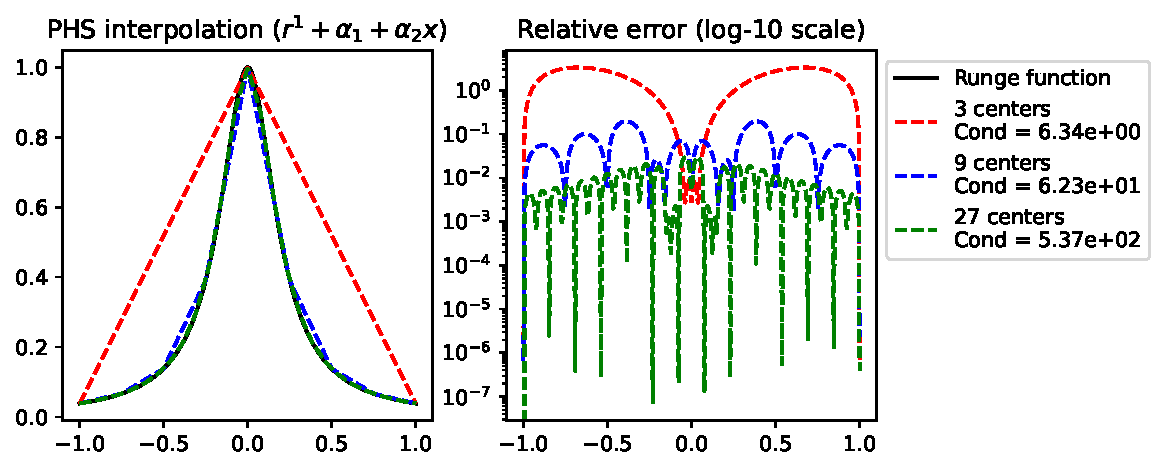
\includegraphics[width=\textwidth]{imagenes/phs_interpolation/runge_phs_r1_deg1.pdf}
  \caption{Left-hand side: PHS interpolation ($r^1$ alongside a linear polynomial). Right-hand side: relative interpolation error.}
  \label{fig:phs-runge-phenomenon-deg-1-discussion}
\end{figure}

\begin{figure}[ht]
  \centering
  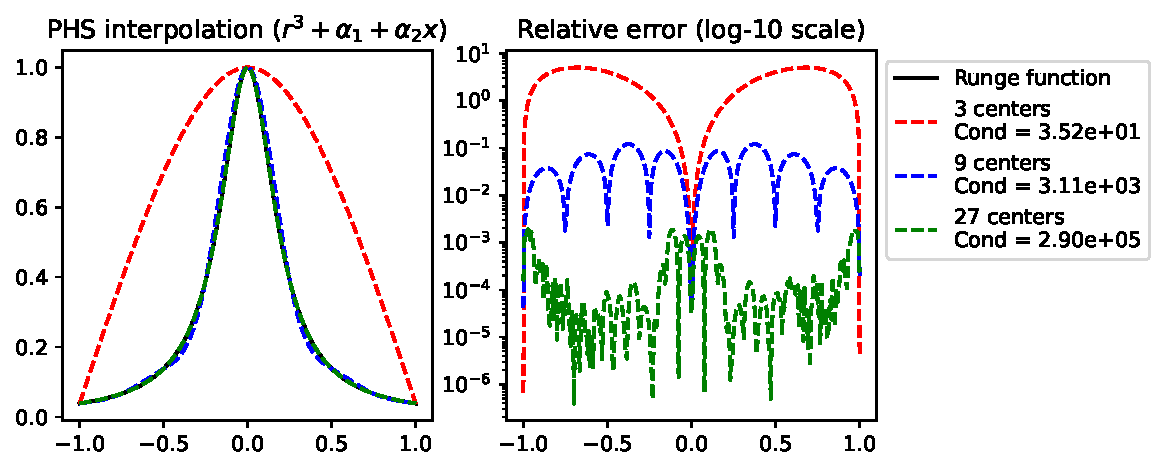
\includegraphics[width=\textwidth]{imagenes/phs_interpolation/runge_phs_r3_deg1.pdf}
  \caption{Left-hand side: PHS interpolation ($r^3$ alongside a linear polynomial). Right-hand side: relative interpolation error.}
  \label{fig:phs-runge-phenomenon-deg-3-discussion}
\end{figure}

% Furthermore, Figures \ref{fig:phs-runge-phenomenon-deg-5} and \ref{fig:phs-runge-phenomenon-deg-7} of the Appendix show that, for $r^5$ and $r^7$, oscillations start appearing when using only 9 equispaced centers. Moreover, the condition numbers start increasing up until the results obtained are completely unreliable.

Another such example of interest is \textbf{Gibbs' phenomenon}\footnote{The following images can be easily derived from the relevant \href{https://github.com/heqro/tfm-experiments/blob/main/introductory_notebooks/rbf_interpolation/gibbs_rbf_and_phs.ipynb}{Gibbs interpolation notebook}.}. Often described in the context of Fourier expansions of piecewise continuously differentiable functions, it establishes that oscillations are bound to occur near such points of non-differentiability (or even jump discontinuity).
Although our techniques do not involve Fourier analysis, the nature of the interpolators we chose (as well as the previous experimentation on Runge's phenomenon) dictate that a similar situation is bound to happen in our framework.

We first consider $x \mapsto \arctan{20x}$, which we promptly depict in Figure \ref{fig:arctan-with-points} for $n=9, 30$ equispaced points. We use as interpolators a polyharmonic spline of the form $\phi(r) = r^3+\alpha_0+\alpha_1 x$ and a Gaussian kernel with shape parameter $\varepsilon=5$.

\begin{figure}[ht]
  \centering
  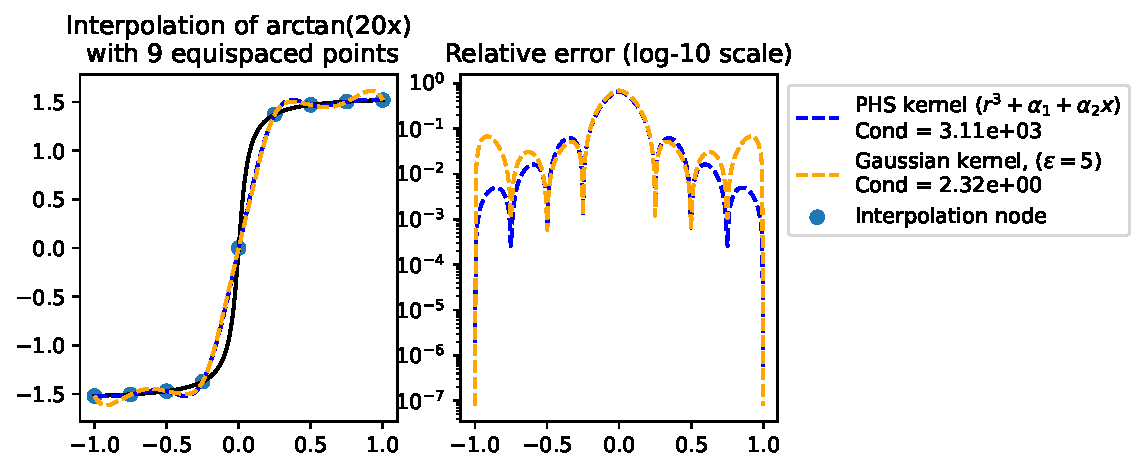
\includegraphics[width=\textwidth]{imagenes/experiments/1d/intro/arctan-with-9-pts.pdf}
  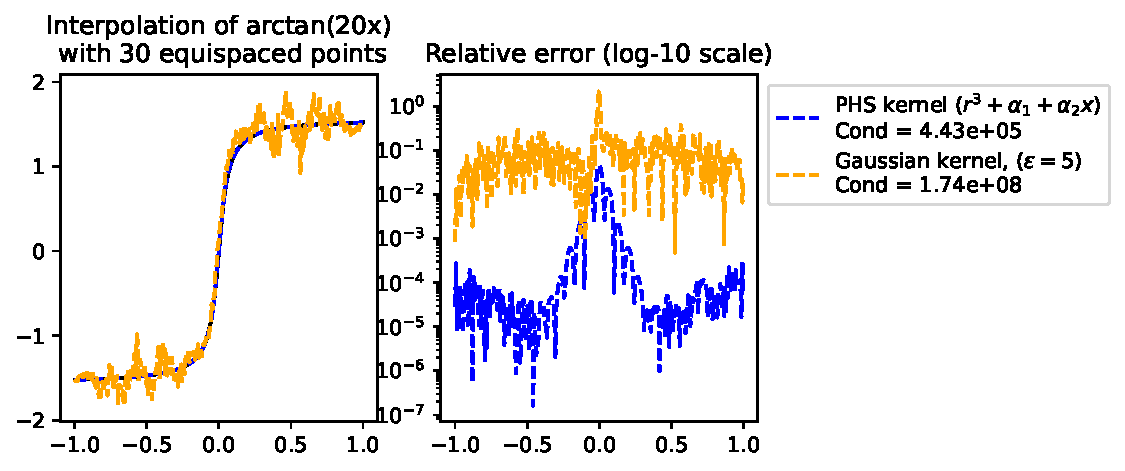
\includegraphics[width=\textwidth]{imagenes/experiments/1d/intro/arctan-with-30-pts.pdf}
  \caption{Top image: interpolation of $\arctan{20x}$ with 9 equispaced points. Bottom image: interpolation of $\arctan{20x}$ with 30 equispaced points. }
  \label{fig:arctan-with-points}
\end{figure}

Strictly speaking, this function we first have considered is not exhibiting the Gibbs' phenomenon as we have defined it. Indeed, for a small sample of points, oscillations are evidently bound to occur as the distance between two consecutive interpolation points is too large for the interpolator. For a larger sample of points, however, oscillations start up by the hand of the ill-conditioning of both interpolation matrices.

\begin{figure}[ht]
  \centering
  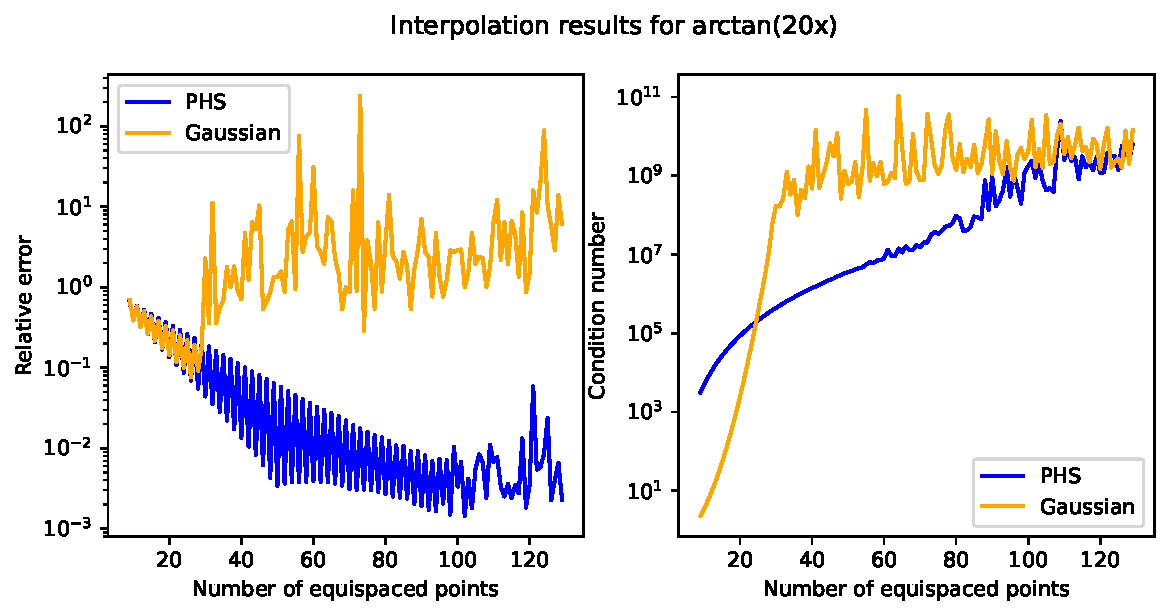
\includegraphics[width=.8\textwidth]{imagenes/experiments/1d/intro/arctan20x-interpolation-curves.pdf}
  \caption{Left-hand side: relative error in the interpolation of $\arctan{20x}$. Right-hand side: condition number of the interpolation matrix.}
  \label{fig:arctan-with-curves}
\end{figure}

Furthermore, Figure \ref{fig:arctan-with-curves} shows that the shape parameter for the Gaussian kernel is not capable of providing any reliable information past the 30 interpolation points, which coincides with the point after which oscillations start showing up for its condition number. On the other hand, the prescribed PHS kernel is capable of providing further accuracy with oscillations in the relative error only showing up past the hundred interpolation points.

In conclusion, even though this particular function does not exhibit Gibbs' phenomenon, it still is an interesting case study for analyzing oscillatory behavior in the Gaussian kernel. Moreover, it is a particular example where this kernel equipped with the proposed shape parameter can only provide a maximum of a digit of accuracy, which highlights again the difficulty of choosing a suitable shape parameter, and how ``one-fits-all'' parameters are unlikely for a varied enough sample of functions.

Gibbs' phenomenon shows up for increasingly larger coefficients of $x$ in $\arctan(20x)$. More specifically, by considering $x\mapsto \arctan(\alpha x)$ for $\alpha \to \infty$ we recover a scaled version of the sign function. Graphs in Figure \ref{fig:sign-with-20-pts} show that the oscillations occur most notably close to the jump due to the change in sign.

\begin{figure}[ht]
  \centering
  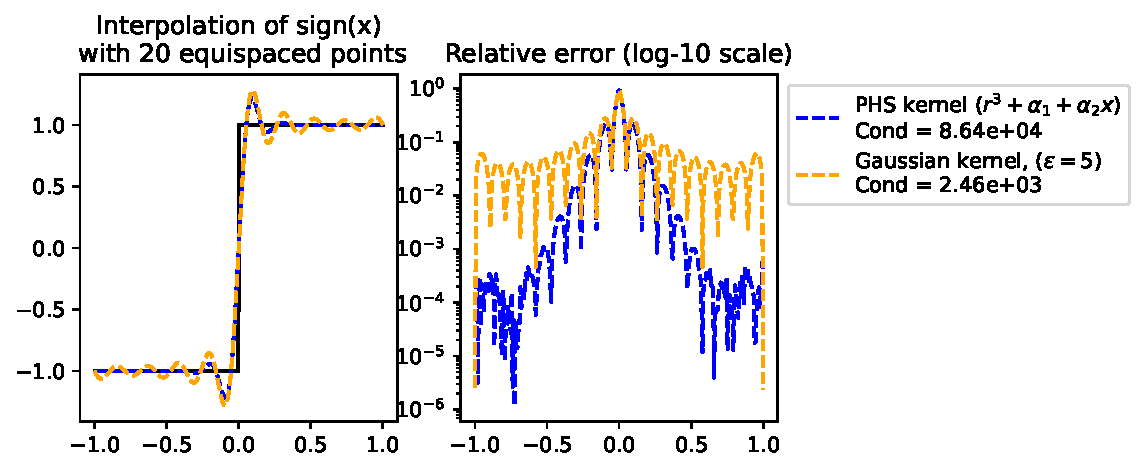
\includegraphics[width=\textwidth]{imagenes/experiments/1d/intro/sign-with-20-pts.pdf}
  \caption{Left-hand side: results of the interpolation of the sign function with 20 equispaced points. Right-hand side: relative error in logarithmic scale.}
  \label{fig:sign-with-20-pts}
\end{figure}

Figure \ref{fig:sign-with-curves} shows a poorer version of the situation shown in previously-analyzed Figure \ref{fig:arctan-with-curves}: even though the number of points where the condition number of the matrices prove to be too large for our problem are similar, neither of the two methods are capable of reducing the $L^\infty-$norm to provide any digit of accuracy in the worst case scenario.

\begin{figure}[ht]
  \centering
  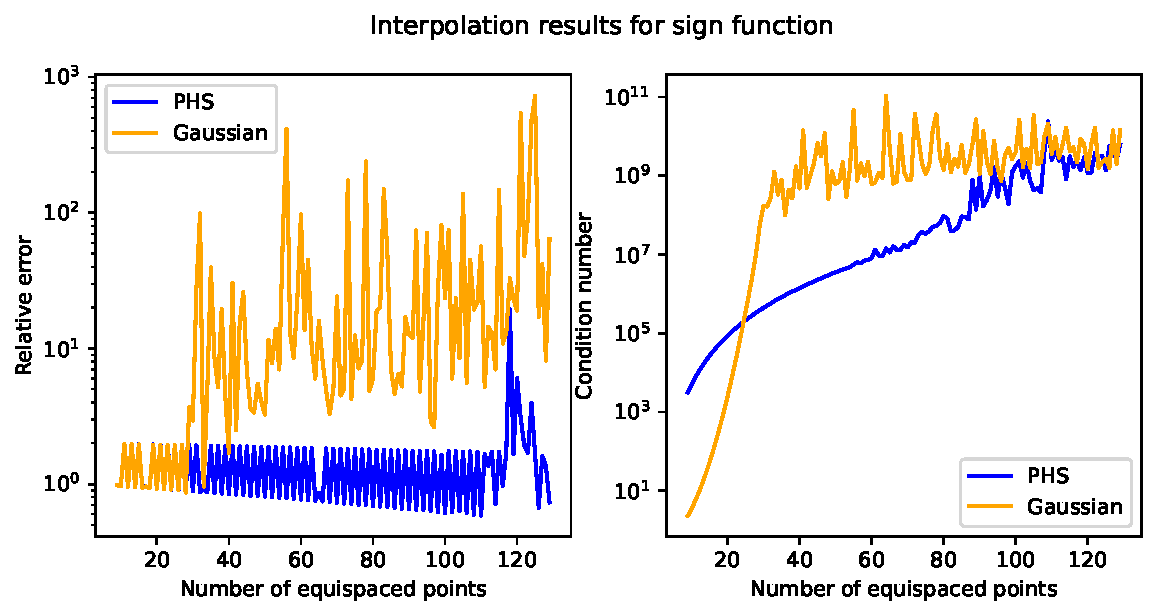
\includegraphics[width=.8\textwidth]{imagenes/experiments/1d/intro/sign-interpolation-curves.pdf}
  \caption{Left-hand side: relative error in the interpolation of the sign function. Right-hand side: condition number for the corresponding interpolation matrix.}
  \label{fig:sign-with-curves}
\end{figure}



\chapter{Preliminary experimentation for methodology development}

% \section*{Hardware information}

All the experimentation featured in the following has been carried out in a server
kindly provided by my advisors.

\begin{table}[h]
  \begin{tabular}{|l|l|}
    \hline
    CPU & $\times 39$ Intel{\textregistered} Xeon{\textregistered} Silver
    4210R @ 2.40 GHz                                                      \\
    \hline
    GPU & NVIDIA RTX A6000 (49140 MiB)                                    \\
    \hline
    RAM & 251 GiB                                                         \\
    \hline
    OS  & Ubuntu 22.04.1 (Kernel 6.5.0-14)                                \\
    \hline
  \end{tabular}
  \caption{Description of the hardware used for experiments and development.}
  \label{tb:hardware-machinery}
\end{table}

\section{Introduction}


The methodology for solving either interpolation problems or differential equations using RBF functions can be expressed in terms of a two-step process:

\begin{itemize}
  \item Explicitly locating the RBF centers and (if applicable) setting the value of the shape parameter $\varepsilon$.
  \item In the case of an interpolation problem, computing the entries of $\hat{\lambda}$ as in \eqref{eqn-p-is-a-linear-combination-of-rbfs}, which ultimately leads to solve \eqref{eqn-linear-system-equations-rbf}. In the case of a differential equation, computing a suitable $\hat{\lambda}$ to satisfy the problem.
\end{itemize}



Alternatively to this methodology, we propose to let the centers as well as the shape parameters\footnote{We remark that we are now speaking in plural.} be found following an \textbf{unsupervised learning} strategy, whereby the training points will not only dictate the values of $\hat{\lambda}$ as in \eqref{eqn-linear-system-equations-rbf}, but also the position of the RBF centers as well as the value of the shape parameters. Relevant pointers in the repository are the following:

\begin{itemize}
  \item The \href{https://github.com/heqro/tfm-experiments/blob/4fd010c560a247b00def20dd94d1f984d7992a24/modules/nn_rbf.py\#L6}{\texttt{RBF\_Free\_All}} class, implementing a Radial Basis Function neural network for an unspecified kernel.
  \item The \href{https://github.com/heqro/tfm-experiments/blob/4fd010c560a247b00def20dd94d1f984d7992a24/modules/nn_poly.py#L6}{\texttt{PolynomialInterpolant}} class, implementing a polynomial function.
  \item The \href{https://github.com/heqro/tfm-experiments/blob/4fd010c560a247b00def20dd94d1f984d7992a24/modules/nn_rbf_poly.py#L8}{\texttt{RBF\_Poly\_Free\_All}} class, whose sole functionality is adding the results of the previous two classes.
\end{itemize}

Denote by $(P)$  an arbitrary $d-$dimensional interpolation problem or differential equation. We will study solutions to $(P)$ in the form of linear combinations of radial basis functions up to a polynomial, say $\mathcal{NN}(\theta) = \mathcal{NN}(\hat{\varepsilon}, \hat{\tmmathbf{x}})$, where $\hat{\varepsilon}$ and $\hat{\tmmathbf{x}}$ denote the (learnable) shape parameters and centers that conform $\varphi$. To lessen the notation, we simply denote by $\mathcal{NN}(\tmmathbf{x})$ the application of $\mathcal{NN}$ to $\tmmathbf{x}$ up to $\hat{\varepsilon}$ and $\hat{\tmmathbf{x}}$.

\subsection{A methodology for finding solutions}

In the case $(P)$ is an interpolation problem, assume we are given $S = \{\tmmathbf{x}_i, \tmmathbf{y}_i\}_{i=1}^n$. Denote by $\mathcal{NN}(S)$ the vector yielding the application of $\mathcal{NN}$ to each $(\tmmathbf{x}_i, \tmmathbf{y}_i)$. In such case, we solve $(P)$ by seeking to minimize the mean-squared error of $\mathcal{NN}(S)$ with respect to $(\tmmathbf{y}_1, \tmmathbf{y}_2, ..., \tmmathbf{y}_n)$. If $(P)$ is instead a differential equation, we then aim to solve a problem of the form \eqref{loss-fun-pinn} following the discussion presented in the corresponding section. Preliminary experimentation showed the Gaussian kernel to be the most suitable kernel to equip to $\mathcal{NN}$, which is the one we refer our experimentation to.

We iteratively minimize the corresponding loss function considering an Adam optimizer alongside a starting learning rate $10^{-2}$. We dynamically modify the learning rate by the action of the \href{https://pytorch.org/docs/stable/generated/torch.optim.lr_scheduler.ReduceLROnPlateau.html}{\texttt{ReduceLROnPlateau}} PyTorch scheduler. It verifies if the loss function took values below \texttt{dynamic\_threshold} in \texttt{patience} iterations:
\begin{itemize}
  \item If that is the case, its internal variable \texttt{dynamic\_threshold} is reduced and we resume operation.
  \item If that is not the case, the learning rate is reduced by \texttt{factor}. If the learning rate is $10^{-6}$, we stop the iterative process.
\end{itemize}

We chose the Adam optimizer to avoid settling on the first local minimum we find for our loss function, especially for the initial values of our dynamic learning rate. Once a suitable local minimum is found, the loss function is observed to start exhibiting oscillations by the action of the Adam optimizer, which the scheduler eventually shuts down. This results in the last hundreds of iterations featuring smooth loss curves: an implicit and ``forced convergence'' to a solution\footnote{Because the proposed loss functions are not observed to be reduced to machine precision, our solution to the interpolation problem should--rigorously speaking--not be called an interpolator, but rather an approximator.}. This strategy has been devised as a compromise between the ``speed'' that comes with a high learning rate and reducing oscillations, most importantly throughout the last iterations.

\subsection{A generic experiment case}

To study the effectiveness of $\mathcal{NN}$ in solving $(P)$, we consider a matrix of experiments indexed by $(C,k)$, where $C$ denotes the number of (initially equispaced) centers we equip $\mathcal{NN}$ with, and $k$ is a scaling factor which will determine the number of training points, say $T$, according to the rule
$T = \lceil \sqrt[d]{C  k} \rceil ^d $.

Furthermore, the training points are uniformly sampled to decisively show the capability of our model to work with an arbitrary set of points. When sampling the training points, we always ensure that some of them are located at the border of the domain. This ensures that $(P)$ is either an interpolation problem (rather than an extrapolation problem) or a well-posed differential equation (so that we have points to work with along the boundary).

For each value of $C$, we compute a starting shape parameter common to all RBFs in the following manner: we first distribute those $C$ centers across an equispaced $d-$dimensional lattice. After that is done, choose $\varepsilon$ such that the condition number of the interpolation problem with interpolation points equal to the centers is between $10^{-6}$ and $10^{-7}$. One can do so, for instance, using the bisection method. For such shapes, the loss function will be observed to steadily decrease while achieving satisfactory performance on the verification dataset. 
\begin{itemize}
  \item Larger starting values of the shape parameter reduce the loss term to the order $10^{-13}$ in few iterations, effectively interpolating the proposed training points. This is observed to harm the ``generalization'' capability of the model, causing large oscillations to occur between any pair of training nodes.
  \item Progressively smaller starting values cause the loss function to stagnate too early for $\mathcal{NN}$ to bear any visual resemblance to the actual function. Furthermore, for small enough values of the starting shape parameter the loss function is observed to oscillate, a clear sign of operating under an ill-conditioned problem.
\end{itemize}

Each experiment configuration $(C,k)$ will be simultaneously solved several times for the following reasons: firstly, the model features a remarkably low amount of parameters, which might make it more susceptible to ``bad'' starting parameter sets. Secondly, to distill those experiments featuring training points that may not lead us to the actual solution of the problem. Thirdly, to observe the performance of our method on a verification dataset which will be common to every experiment. Finally, to elaborate statistic descriptions of the model's parameters: shape parameter, coefficients and centers. Some recurrent questions to answer will be the following:

\begin{itemize}
  \item How do the $L^\infty$ and $L^2-$norms on the verification dataset behave as $C$ and $k$ increase?
  \item Do we observe any improvements when equipping a polynomial term to our RBF?
  % \item What about the GPU memory consumed by each $(C,k)$?
  \item Are there any recurrent distribution of centers, shape parameters or coefficients?
\end{itemize}

The question for execution times is a relevant one as well, albeit it cannot be reliably answered as the experiments are launched in a shared server, that is, measurements have been carried out but they have been observed to be inconsistent, varying according to the workload of the server during the launch event.

One reasonable concern for solving any experiment several simultaneous times is exhausting the computing resources of the server, namely CPU and GPU. The multiple processors the server features is enough to quell the CPU concern as long as we launch fewer instances than the amount of idle processors. 

On the other hand, model memory allocation problem is often an issue when dealing with PINNs, which we address in the following by turning to the \href{https://pytorch.org/docs/stable/generated/torch.cuda.max_memory_allocated.html}{\texttt{max\_memory\_allocated()}}
method of the \texttt{torch.cuda} namespace in Python. This method returns the peak allocated memory (in bytes) since the beginning of the program. Therefore, this
measurement is to be regarded as approximate. Figure \ref{fig:model-consumption-memory} depicts the memory consumption of the
model for different numbers of centers per dimension. It is observed to reach $100$ MB for the largest pair of dimensionality and centers we evaluate, two orders of magnitude below the amount the server can allocate. For our purposes, the model is not going to be an issue regarding GPU memory.

The memory consumed by each instance is not going to be that small. The training and validation datasets are observed to be larger contributors to the total allocated memory. Regardless, the memory they occupy in low dimensions is observed to be negligible in comparison to the memory occupied by the CUDA context\footnote{Recall that the CUDA context manages the interaction between PyTorch tensors and CUDA-capable devices (usually GPUs). The CUDA context in PyTorch handles memory allocation, device synchronization, and execution of CUDA operations on tensors stored on GPU devices. For each separate process, a CUDA context is invoked, which may be a problem if a large amount of ML problems featuring large models are to be solved simultaneously  (refer for instance to \href{https://github.com/pytorch/pytorch/issues/20532}{previous GitHub discussions} in PyTorch's repository).}.


\begin{figure}
  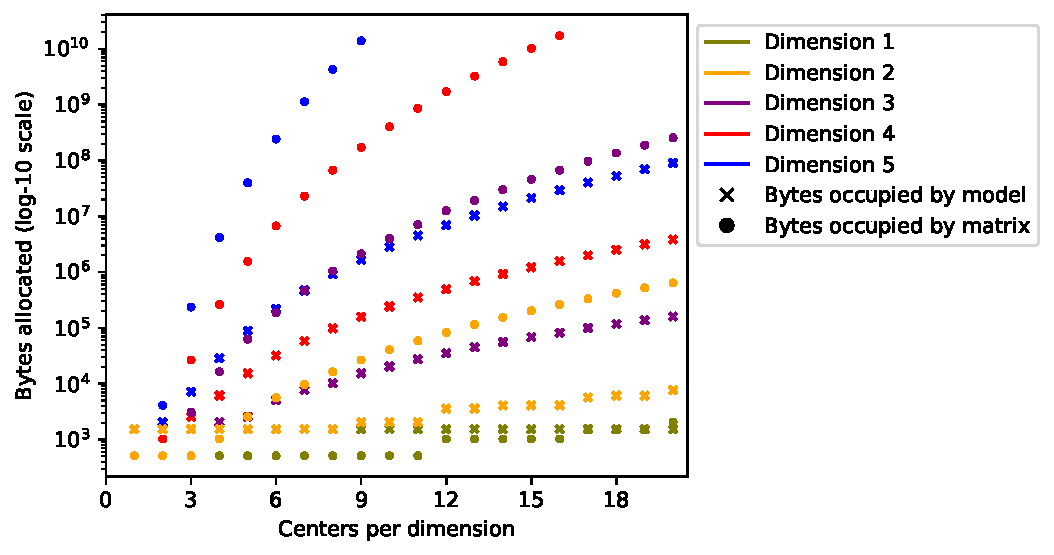
\includegraphics[width=.7\textwidth]{imagenes/model_consumption/Memory_allocation_vs_number_of_centers_per_dimension.pdf}
  \caption{Memory allocation of the model plotted against the number of centers per dimension.}
  \label{fig:model-consumption-memory}
\end{figure}

In the following, we will work on ``well-behaved'' polynomial functions. Our objective is to evaluate the performance of our model when we expect to the performance to improve when explicitly incorporating polynomial terms. %We will present the results in graphic form, using vector images to allow the usage of electronic zoom if further interpretation of the representations is of interest to the reader.

\section{Approximation of functions}



\subsection*{One-dimensional case}

We consider the function $x \mapsto u_2(x)=(x-1/2)^2$ for $x \in [-1,1]$. We may refer to this function by \texttt{u2} as well. For this interval, we have found suitable starting shape parameters $(0.78125, 1.5625, 2.5, 3.6621, 5.6152)$, which we map to the list of (initially equispaced) centers $(7,11,15,20,30)$, respectively.

Figure \ref{u2-example-training-TR15-C15} shows how an instance of this experiment is carried out. Notice (top-right image) that the largest error is located where the density of training points is at its lowest. Furthermore, the two figures on the left-hand show the location and the shape parameters of the RBF functions, allowing one to see at a glance the parameters of the proposed network. Finally, the image on the bottom-right hand side shows the loss function of our model alongside the $L^2$ and $L^\infty-$norms on the verification dataset. The action of the scheduler allows us to iteratively reduce oscillations in the model, most importantly nullifying them in the very last few iterations.

\begin{figure}
  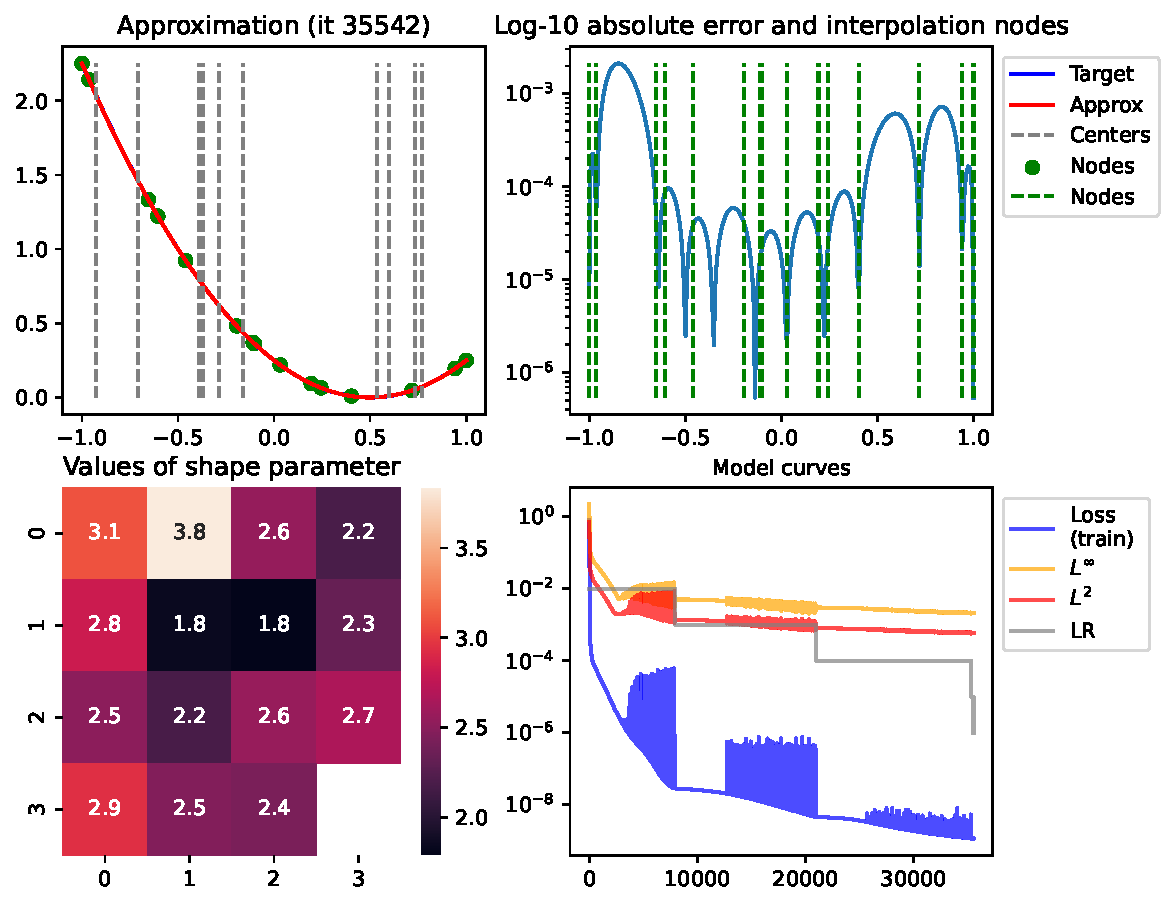
\includegraphics[width=\textwidth]{imagenes/experiments/1d/statistical_1d_full_scheduler_interpolation/u2-TR15-C15-Kgaussian_kernel-Sh2.5-6-E35542.pdf}
  \caption{Last iteration of an instance of the approximation experiment $(C,k)=(15,1)$ for $u_2$ with no polynomial term. Top-left: original function alongside its approximation, the training nodes and the centers. Top-right: absolute error alongside the training nodes. Bottom-left: values of each of the shape parameters of our RBFs. Bottom-right: model curves, namely the loss term and learning rates, as well as the $L^\infty$ and $L^2$ norms on the verification datasets.}
  \label{u2-example-training-TR15-C15}
\end{figure}

As previously anticipated, we shall be repeating each experiment configuration several times to extract statistics on the performance of our model, most importantly when a polynomial term is considered. Figure \ref{fig:u2-results-overall-poly-1} shows a comparison of the distribution of results in the $L^\infty$ and $L^2-$norms as well as in execution times, when no polynomial term is considered. We observe that the results improve more visibly when $k$ is increased than when $C$ is increased, which is likely to the ``good behavior'' of the test function. The consideration of a quadratic polynomial term further decreases the $L^2$ and $L^\infty-$norm metrics, most notably for $C=7$. We observe a similar situation in Figure \ref{fig:u2-results-overall-poly2}, which presents the same results albeit when considering a quadratic polynomial addend.

\clearpage
\begin{sidewaysfigure}[H]
  \hspace*{-1cm}
  \begin{tabular}{cccccc}
    {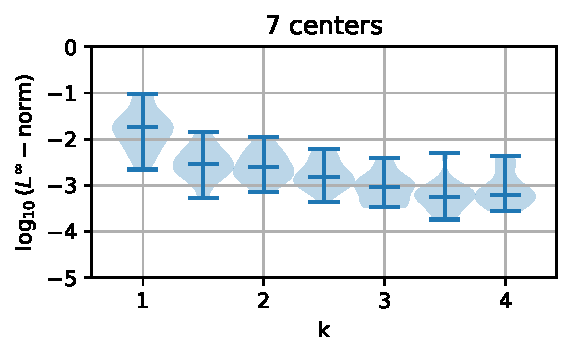
\includegraphics[width=.014\textwidth,clip=true,trim={0 .59cm 9cm 0}]{imagenes/experiments/1d/statistical_1d_full_scheduler_interpolation/violins/violins_linf_u2_C7_gaussian_kernel_shape_0.78125_Poly-1.pdf}} & {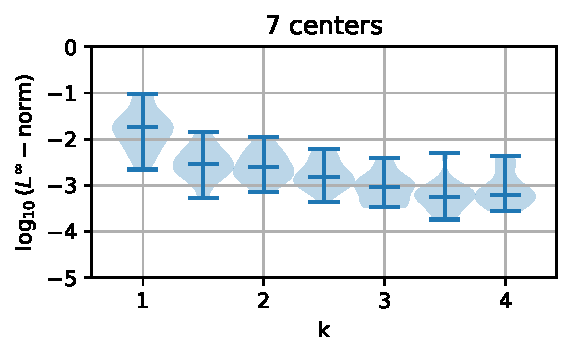
\includegraphics[width=.2\textwidth,clip=true,trim={.81cm .59cm 0 0}]{imagenes/experiments/1d/statistical_1d_full_scheduler_interpolation/violins/violins_linf_u2_C7_gaussian_kernel_shape_0.78125_Poly-1.pdf}}   & 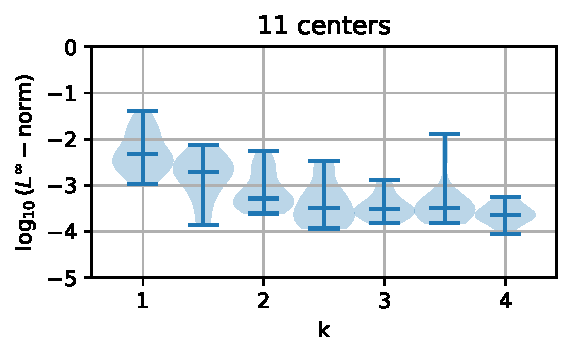
\includegraphics[width=.2\textwidth,clip=true,trim={.81cm .59cm 0 0}]{imagenes/experiments/1d/statistical_1d_full_scheduler_interpolation/violins/violins_linf_u2_C11_gaussian_kernel_shape_1.5625_Poly-1.pdf}   & 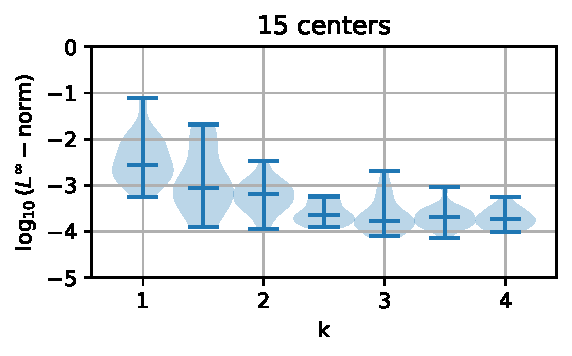
\includegraphics[width=.2\textwidth,clip=true,trim={.81cm .59cm 0 0}]{imagenes/experiments/1d/statistical_1d_full_scheduler_interpolation/violins/violins_linf_u2_C15_gaussian_kernel_shape_2.5_Poly-1.pdf}   & 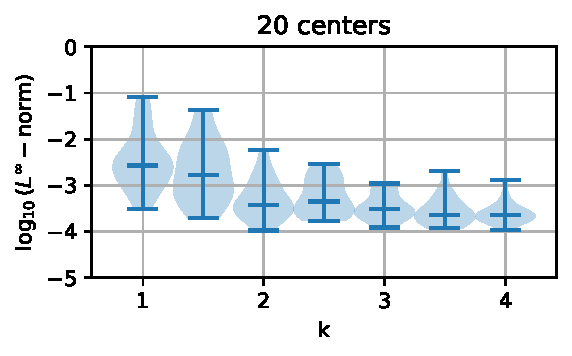
\includegraphics[width=.2\textwidth,clip=true,trim={.81cm .59cm 0 0}]{imagenes/experiments/1d/statistical_1d_full_scheduler_interpolation/violins/violins_linf_u2_C20_gaussian_kernel_shape_3.6621_Poly-1.pdf}   & 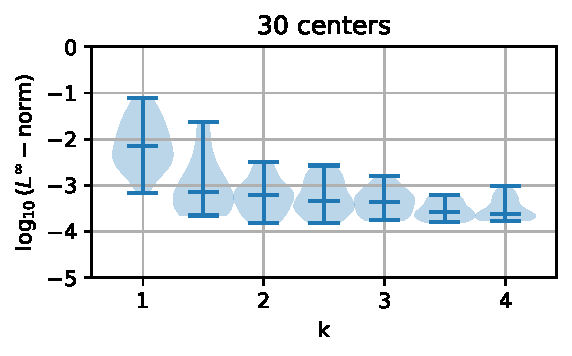
\includegraphics[width=.2\textwidth,clip=true,trim={.81cm .59cm 0 0}]{imagenes/experiments/1d/statistical_1d_full_scheduler_interpolation/violins/violins_linf_u2_C30_gaussian_kernel_shape_5.6152_Poly-1.pdf}   \\
    {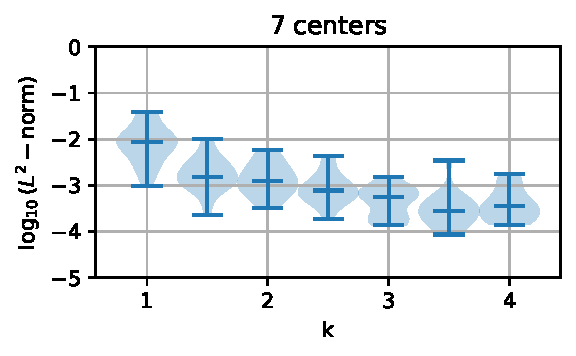
\includegraphics[width=.014\textwidth,clip=true,trim={0 .59cm 9cm 0}]{imagenes/experiments/1d/statistical_1d_full_scheduler_interpolation/violins/violins_l2_u2_C7_gaussian_kernel_shape_0.78125_Poly-1.pdf}}   & {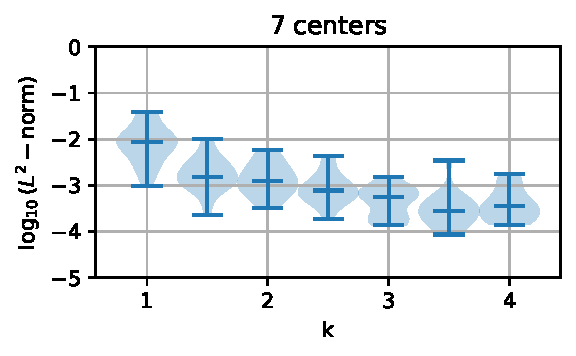
\includegraphics[width=.2\textwidth,clip=true,trim={.81cm .59cm 0 .65cm}]{imagenes/experiments/1d/statistical_1d_full_scheduler_interpolation/violins/violins_l2_u2_C7_gaussian_kernel_shape_0.78125_Poly-1.pdf}} & 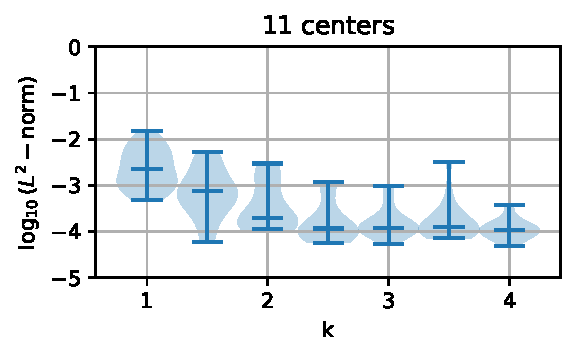
\includegraphics[width=.2\textwidth,clip=true,trim={.81cm .59cm 0 .65cm}]{imagenes/experiments/1d/statistical_1d_full_scheduler_interpolation/violins/violins_l2_u2_C11_gaussian_kernel_shape_1.5625_Poly-1.pdf} & 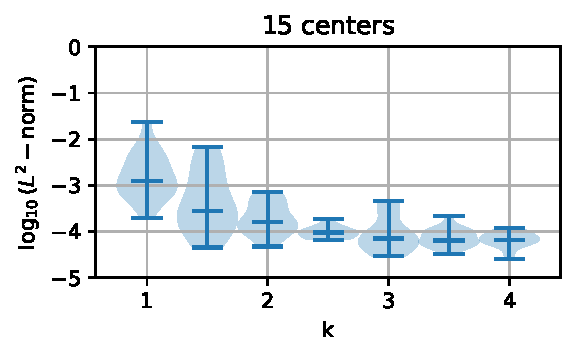
\includegraphics[width=.2\textwidth,clip=true,trim={.81cm .59cm 0 .65cm}]{imagenes/experiments/1d/statistical_1d_full_scheduler_interpolation/violins/violins_l2_u2_C15_gaussian_kernel_shape_2.5_Poly-1.pdf} & 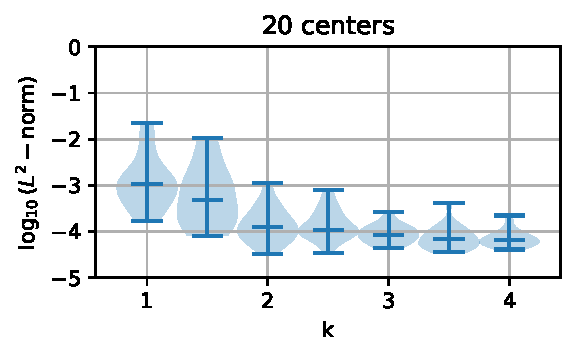
\includegraphics[width=.2\textwidth,clip=true,trim={.81cm .59cm 0 .65cm}]{imagenes/experiments/1d/statistical_1d_full_scheduler_interpolation/violins/violins_l2_u2_C20_gaussian_kernel_shape_3.6621_Poly-1.pdf} & 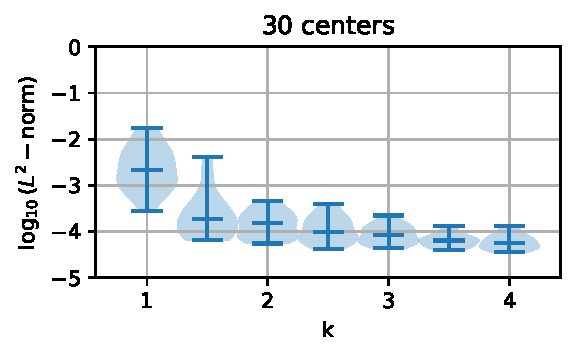
\includegraphics[width=.2\textwidth,clip=true,trim={.81cm .59cm 0 .65cm}]{imagenes/experiments/1d/statistical_1d_full_scheduler_interpolation/violins/violins_l2_u2_C30_gaussian_kernel_shape_5.6152_Poly-1.pdf} \\
    % {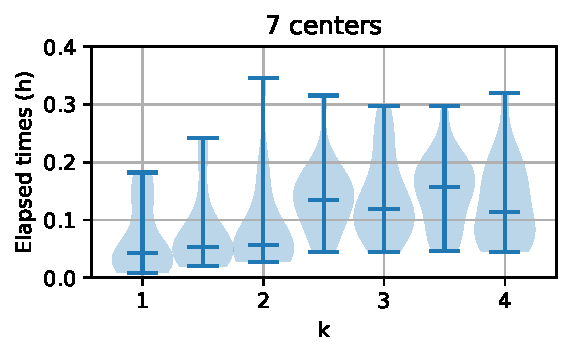
\includegraphics[width=.014\textwidth,clip=true,trim={0 0 9cm 0}]{imagenes/experiments/1d/statistical_1d_full_scheduler_interpolation/violins/violins_times_u2_C7_gaussian_kernel_shape_0.78125_Poly-1.pdf}}    & {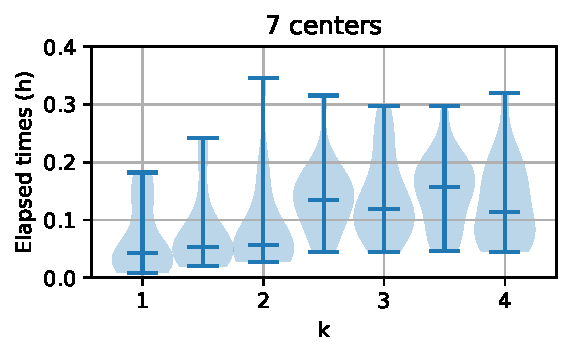
\includegraphics[width=.2\textwidth,clip=true,trim={.81cm 0 0 .65cm}]{imagenes/experiments/1d/statistical_1d_full_scheduler_interpolation/violins/violins_times_u2_C7_gaussian_kernel_shape_0.78125_Poly-1.pdf}}   & 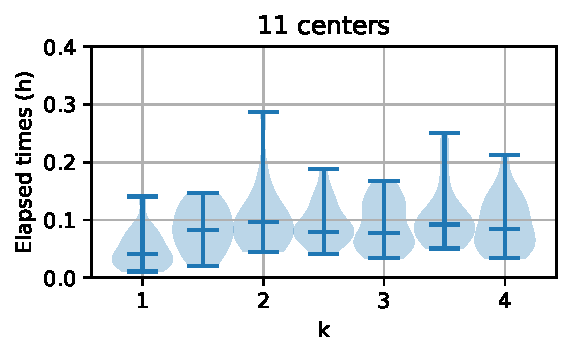
\includegraphics[width=.2\textwidth,clip=true,trim={.81cm 0 0 .65cm}]{imagenes/experiments/1d/statistical_1d_full_scheduler_interpolation/violins/violins_times_u2_C11_gaussian_kernel_shape_1.5625_Poly-1.pdf} & 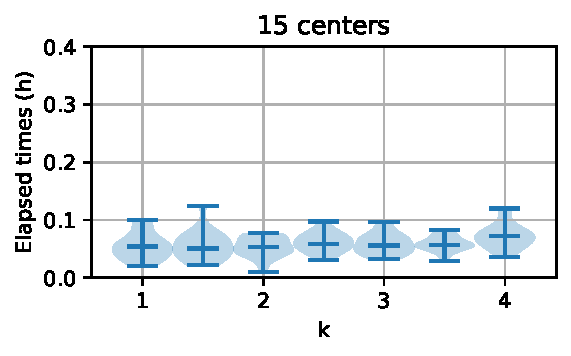
\includegraphics[width=.2\textwidth,clip=true,trim={.81cm 0 0 .65cm}]{imagenes/experiments/1d/statistical_1d_full_scheduler_interpolation/violins/violins_times_u2_C15_gaussian_kernel_shape_2.5_Poly-1.pdf} & 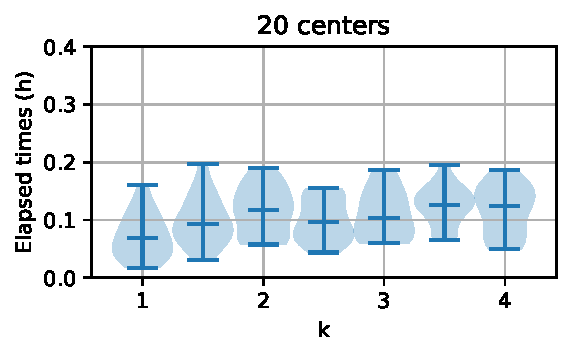
\includegraphics[width=.2\textwidth,clip=true,trim={.81cm 0 0 .65cm}]{imagenes/experiments/1d/statistical_1d_full_scheduler_interpolation/violins/violins_times_u2_C20_gaussian_kernel_shape_3.6621_Poly-1.pdf}  & 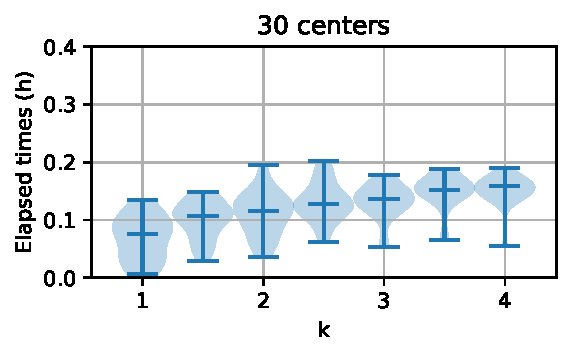
\includegraphics[width=.2\textwidth,clip=true,trim={.81cm 0 0 .65cm}]{imagenes/experiments/1d/statistical_1d_full_scheduler_interpolation/violins/violins_times_u2_C30_gaussian_kernel_shape_5.6152_Poly-1.pdf} 
  \end{tabular}
  % \includegraphics[width=\textwidth]{figure.png}
  \caption{Distribution of the $L^\infty$, $L^2-$norms on our verification dataset
    % , and overall elapsed times, 
    without a polynomial term.}
  \label{fig:u2-results-overall-poly-1}
\end{sidewaysfigure}


% \clearpage
\begin{sidewaysfigure}[H]
  \hspace*{-1cm}
  \begin{tabular}{cccccc}
    {\includegraphics[width=.014\textwidth,clip=true,trim={0 .59cm 9cm 0}]{imagenes/experiments/1d/statistical_1d_full_scheduler_interpolation/violins/violins_linf_u2_C7_gaussian_kernel_shape_0.78125_Poly2.pdf}} & {\includegraphics[width=.2\textwidth,clip=true,trim={.81cm .59cm 0 0}]{imagenes/experiments/1d/statistical_1d_full_scheduler_interpolation/violins/violins_linf_u2_C7_gaussian_kernel_shape_0.78125_Poly2.pdf}}   & \includegraphics[width=.2\textwidth,clip=true,trim={.81cm .59cm 0 0}]{imagenes/experiments/1d/statistical_1d_full_scheduler_interpolation/violins/violins_linf_u2_C11_gaussian_kernel_shape_1.5625_Poly2.pdf}   & \includegraphics[width=.2\textwidth,clip=true,trim={.81cm .59cm 0 0}]{imagenes/experiments/1d/statistical_1d_full_scheduler_interpolation/violins/violins_linf_u2_C15_gaussian_kernel_shape_2.5_Poly2.pdf}   & \includegraphics[width=.2\textwidth,clip=true,trim={.81cm .59cm 0 0}]{imagenes/experiments/1d/statistical_1d_full_scheduler_interpolation/violins/violins_linf_u2_C20_gaussian_kernel_shape_3.6621_Poly2.pdf}   & \includegraphics[width=.2\textwidth,clip=true,trim={.81cm .59cm 0 0}]{imagenes/experiments/1d/statistical_1d_full_scheduler_interpolation/violins/violins_linf_u2_C30_gaussian_kernel_shape_5.6152_Poly2.pdf}   \\
    {\includegraphics[width=.014\textwidth,clip=true,trim={0 .59cm 9cm 0}]{imagenes/experiments/1d/statistical_1d_full_scheduler_interpolation/violins/violins_l2_u2_C7_gaussian_kernel_shape_0.78125_Poly2.pdf}}   & {\includegraphics[width=.2\textwidth,clip=true,trim={.81cm .59cm 0 .65cm}]{imagenes/experiments/1d/statistical_1d_full_scheduler_interpolation/violins/violins_l2_u2_C7_gaussian_kernel_shape_0.78125_Poly2.pdf}} & \includegraphics[width=.2\textwidth,clip=true,trim={.81cm .59cm 0 .65cm}]{imagenes/experiments/1d/statistical_1d_full_scheduler_interpolation/violins/violins_l2_u2_C11_gaussian_kernel_shape_1.5625_Poly2.pdf} & \includegraphics[width=.2\textwidth,clip=true,trim={.81cm .59cm 0 .65cm}]{imagenes/experiments/1d/statistical_1d_full_scheduler_interpolation/violins/violins_l2_u2_C15_gaussian_kernel_shape_2.5_Poly2.pdf} & \includegraphics[width=.2\textwidth,clip=true,trim={.81cm .59cm 0 .65cm}]{imagenes/experiments/1d/statistical_1d_full_scheduler_interpolation/violins/violins_l2_u2_C20_gaussian_kernel_shape_3.6621_Poly2.pdf} & \includegraphics[width=.2\textwidth,clip=true,trim={.81cm .59cm 0 .65cm}]{imagenes/experiments/1d/statistical_1d_full_scheduler_interpolation/violins/violins_l2_u2_C30_gaussian_kernel_shape_5.6152_Poly2.pdf} \\
    % {\includegraphics[width=.014\textwidth,clip=true,trim={0 0 9cm 0}]{imagenes/experiments/1d/statistical_1d_full_scheduler_interpolation/violins/violins_times_u2_C7_gaussian_kernel_shape_0.78125_Poly2.pdf}}    & {\includegraphics[width=.2\textwidth,clip=true,trim={.81cm 0 0 .65cm}]{imagenes/experiments/1d/statistical_1d_full_scheduler_interpolation/violins/violins_times_u2_C7_gaussian_kernel_shape_0.78125_Poly2.pdf}}   & \includegraphics[width=.2\textwidth,clip=true,trim={.81cm 0 0 .65cm}]{imagenes/experiments/1d/statistical_1d_full_scheduler_interpolation/violins/violins_times_u2_C11_gaussian_kernel_shape_1.5625_Poly2.pdf} & \includegraphics[width=.2\textwidth,clip=true,trim={.81cm 0 0 .65cm}]{imagenes/experiments/1d/statistical_1d_full_scheduler_interpolation/violins/violins_times_u2_C15_gaussian_kernel_shape_2.5_Poly2.pdf} & \includegraphics[width=.2\textwidth,clip=true,trim={.81cm 0 0 .65cm}]{imagenes/experiments/1d/statistical_1d_full_scheduler_interpolation/violins/violins_times_u2_C20_gaussian_kernel_shape_3.6621_Poly2.pdf}  & \includegraphics[width=.2\textwidth,clip=true,trim={.81cm 0 0 .65cm}]{imagenes/experiments/1d/statistical_1d_full_scheduler_interpolation/violins/violins_times_u2_C30_gaussian_kernel_shape_5.6152_Poly2.pdf} 
  \end{tabular}
  % \includegraphics[width=\textwidth]{figure.png}
  \caption{Distribution of the $L^\infty$, $L^2-$norms on our verification dataset
    % , and overall elapsed times, 
    with a quadratic polynomial term (bottom section).}
  \label{fig:u2-results-overall-poly2}
\end{sidewaysfigure}

A reasonable concern comes from the fact that letting the iterative process run long enough might eventually allow for oscillations to arise between any two training nodes. To settle this problem, Figure \ref{fig:u2-results-incidence-l-norms} depicts, across all instances of experiments, the incidence of the $L^\infty$ and $L^2-$norms during the last iteration in comparison to the best iteration in the $L^\infty-$norm that was hit. It indicates that the last iterations we make are, in general, not far from the best iterations, sometimes even surpassing the best iteration for the $L^2-$norm.

\begin{figure}
  \hspace*{-2cm}
  \begin{tabular}{cc}
    \includegraphics[width=.6\textwidth]{imagenes/experiments/1d/statistical_1d_full_scheduler_interpolation/incidence_of_linf.pdf}
    \includegraphics[width=.6\textwidth]{imagenes/experiments/1d/statistical_1d_full_scheduler_interpolation/incidence_of_l2.pdf}
  \end{tabular}
  \caption{Left: incidence of the $L^\infty-$norm across all experiments, comparing the optimum iteration in this value with the last iteration. Right: incidence of the $L^2-$norm across all experiments, comparing with the value that produced the best iteration in the $L^\infty-$norm.}
  \label{fig:u2-results-incidence-l-norms}
\end{figure}

Figure \ref{fig:u2-results-largest-error} features two diagrams of the averages of the absolute errors across all training experiments that have been carried out, most importantly the cases $k=1$ and $k=4$. In coherence with Figures \ref{fig:u2-results-overall-poly-1} and \ref{fig:u2-results-overall-poly2}, it indicates that the case $k=4$ produces the best results: $(C,k)=(7,4)$ is observed to produce comparable results to the case $(C,k)=(30,1)$, indicating that the results improve with the number of training points.

\begin{figure}
  \includegraphics[width=\textwidth]{imagenes/experiments/1d/statistical_1d_full_scheduler_interpolation/u2_30_1}
  \includegraphics[width=\textwidth]{imagenes/experiments/1d/statistical_1d_full_scheduler_interpolation/u2_30_4}
  \caption{Average of the absolute errors across all training experiments, comparing the cases $k=1$ and $k=4$.}
  \label{fig:u2-results-largest-error}
\end{figure}

Figure \ref{fig:u2-results-shape-parameters} depicts the incidence of the shape parameters at the end of all training processes fitted to a normal distribution. Some observations are in order:
\begin{itemize}
  \item The mean of the fitted normal distributions approach the starting shape parameter as $C$ (and thus the starting parameter) is increased. The fitted variance diminishes as well.
  \item For $\varepsilon=0.78125$, associated with $C=7$, some shape parameters are found to be close to zero. This indicates that some RBF addends are effectively working as bias terms. This is observed not to happen for larger values of $C$.
\end{itemize}

\begin{figure}
  \includegraphics[width=\textwidth]{imagenes/experiments/1d/statistical_1d_full_scheduler_interpolation/distribution_of_shape_parameters_at_end_of_training.pdf}
  \caption{Distribution of shape parameters at the end of the training process fitted to a normal distribution.}
  \label{fig:u2-results-shape-parameters}
\end{figure}

Figure \ref{fig:u2-results-all} provides cursory insights into the learning curves of the model. It features the loss functions and the $L^2$ and $L^\infty-$norms of all the experiments that have been carried out. It shows that the loss term reaches satisfactory orders of magnitude, well under $10^{-5}$. Furthermore, it also shows that the $L^2$ and $L^\infty-$norms have similar behaviors, differing only in slight visual details.

\begin{figure}[h]
  \includegraphics[width=.7\textwidth]{imagenes/experiments/1d/statistical_1d_full_scheduler_interpolation/Loss_curves_semilogy_all.png}
  \includegraphics[width=.7\textwidth]{imagenes/experiments/1d/statistical_1d_full_scheduler_interpolation/L2_curves_semilogy_all.png}
  \includegraphics[width=.7\textwidth]{imagenes/experiments/1d/statistical_1d_full_scheduler_interpolation/Linf_curves_semilogy_all.png}
  \caption{Representation of the loss, $L^2$ and $L^\infty$ curves across all iterations.}
  \label{fig:u2-results-all}
\end{figure}


Figure \ref{fig:u2-results-shapes-etc-c30-tr120} depicts a histogram of the trained centers by the end of all training instances, alongside violin plots of the shapes and coefficients. This is the experiment featuring the largest amount of centers and training points. Some immediate observations about this Figure are the following: \begin{itemize}
  \item There the largest incidence of centers is located \textit{outside} the domain of the problem.
  \item The medians of the coefficients, depicted by the horizontal lines in the violin plots, seem to match the behavior of the actual function.
\end{itemize}

The same diagrams can be drawn for different pairs $(C,k)$, and the same observations will be reached. However, there are some key differences: the incidence of centers is further away from the domain as less centers are taken into consideration, and the coefficients do not resemble the function as closely as Figure \ref{fig:u2-results-shapes-etc-c30-tr120}, the resemblance loosening as fewer centers are considered.

\begin{figure}
  \includegraphics[width=\textwidth]{imagenes/experiments/1d/statistical_1d_full_scheduler_interpolation/C30-TR120-u2.pdf}
  \caption{Top diagram: histogram of the incidence of centers at the end of all the training processes, alongside \texttt{u2}. Middle diagram: violin plots of the shape parameter for each histogram bin. Bottom: violin plots of the coefficients for each histogram bin.}
  \label{fig:u2-results-shapes-etc-c30-tr120}
\end{figure}



\clearpage
\subsection*{Two-dimensional case}

We consider the function $(x,y) \mapsto (x-1/2)^2 + (y-1/2)^2$ for $(x,y)$ in the disk centered in $(0,0)$ of unit radius. We may refer to this function as \texttt{parabola}. Considering initially equispaced centers in the interval $[-1,1]\times[-1,1]$, we found suitable starting shape parameters $\{1.3428, 1.9531, 2.5635, 3.1738, 3.6621\}$. They will be tied to $C=\{7^2,9^2,11^2,13^2,15^2\}$, respectively.

One can sample uniformly-distributed training points for working with the unitary disk as follows:
\begin{itemize}
  \item The interior points are sampled uniformly on the interval $[-1,1]\times[-1,1]$. We retain those verifying the equation of the disk.
  \item The points on the boundary have to be explicitly generated, as the boundary constitutes a measure zero set in 2D. We obtain them by sampling from the uniform distribution $U[0,2\pi)$, and then identifying $(x,y)=(\cos\theta, \sin\theta)$.
\end{itemize}

Figure \ref{fig:uniform-circle} visually depicts the sieve of points that is carried out when sampling from the uniform distribution (points in green and blue), while also showing the generic formulation to generate points at the boundary (point in orange).

\begin{figure}[h]
  {\includegraphics[width=.8\textwidth]{imagenes/experiments/helpful_images/uniform_circle.pdf}}
  \caption{Visual representation of one can generate uniformly distributed points as well as points lying on the boundary of a circle.}
  \label{fig:uniform-circle}
\end{figure}

Working in the interior, it is not correct to sample $r$ from $U[0,1)$ and $\theta$ from $U[0,2\pi)$ and then map $(x,y)=(r \cos \theta, r \sin \theta)$. The change to polar coordinates is not a linear function; for our purposes, this implies that regions close to the origin will feature a higher density of points than those farther from it.

For the sake of reproducibility, we explicitly state the number of points we consider on the boundary and inside the circle: let $T^2$ be the number of training points we work with. We then consider $4 (T - 2) + 4$ points on the boundary, and the rest are to be in the interior of the domain\footnote{This apparently obscure formula comes from the idea that, working with a square, a reasonable amount of boundary points is $T$ per side. Provided one would like to always have points at the corners of the square, one would then have $T-2$ uniformly sampled points per side (because of the $2$ fixed points), which yields our proposed formula for the number of points on the boundary.}.

Much like in the one-dimensional case, Figure \ref{fig:parabola-example-training-TR15-C81} depicts a particular instance of this experiment. The metrics of the model (right-hand side) show that the scheduler readily reduces oscillations, reducing the learning rate as soon as they show up. In comparison with the one-dimensional case, the oscillations are much shorter-lived. For this instance of the experiment, the learning rate that occupies most of the time of computation is $10^{-5}$. Note that a notable amount of centers is outside the domain of our data.

\begin{figure}[h]
  \includegraphics[width=\textwidth]{imagenes/experiments/2d/statistical_2d_full_scheduler_interpolation/parabola/parabola-TR15-C81-Kgaussian_kernel-Sh1.9531-rrrepetishon-E60521.pdf}
  \caption{Last iteration of an instance of the approximation experiment $(C,k)=(81,2.5)$. Left-hand side: absolute error on the verification dataset. Right-hand side: model curves of the training process (loss function, learning rate) as well as its performance on the verification dataset ($L^2, L^\infty-$norms).}
  \label{fig:parabola-example-training-TR15-C81}
\end{figure}




In the following, we show the comparison of the distribution of these results in the $L^\infty$ and $L^2-$norms and in execution times, without (Figure \ref{fig:parabola-results-overall-poly-1}) and with a quadratic polynomial addend (Figure \ref{fig:parabola-results-overall-poly2}). As observed in the 1D case, the improvements come not from the consideration of a larger value of $C$, but rather by the increment of $k$. Increasing $k$ is also seen to visibly decrease the spread of results in the $L^2$ and $L^\infty-$norms. The consideration of a quadratic polynomial produces timid improvements on these two metrics. %Finally, the execution times are at their largest for increasing values of $C$.
\clearpage
\begin{sidewaysfigure}[H]
  \hspace*{-1cm}
  \begin{tabular}{cccccc}
    {\includegraphics[width=.014\textwidth,clip=true,trim={0 .59cm 9cm 0}]{imagenes/experiments/2d/statistical_2d_full_scheduler_interpolation/parabola/violins/violins_linf_parabola_C49_gaussian_kernel_shape_1.3428_Poly-1.pdf}} & {\includegraphics[width=.2\textwidth,clip=true,trim={.81cm .59cm 0 0}]{imagenes/experiments/2d/statistical_2d_full_scheduler_interpolation/parabola/violins/violins_linf_parabola_C49_gaussian_kernel_shape_1.3428_Poly-1.pdf}}   & \includegraphics[width=.2\textwidth,clip=true,trim={.81cm .59cm 0 0}]{imagenes/experiments/2d/statistical_2d_full_scheduler_interpolation/parabola/violins/violins_linf_parabola_C81_gaussian_kernel_shape_1.9531_Poly-1.pdf}   & \includegraphics[width=.2\textwidth,clip=true,trim={.81cm .59cm 0 0}]{imagenes/experiments/2d/statistical_2d_full_scheduler_interpolation/parabola/violins/violins_linf_parabola_C121_gaussian_kernel_shape_2.5635_Poly-1.pdf}   & \includegraphics[width=.2\textwidth,clip=true,trim={.81cm .59cm 0 0}]{imagenes/experiments/2d/statistical_2d_full_scheduler_interpolation/parabola/violins/violins_linf_parabola_C169_gaussian_kernel_shape_3.1738_Poly-1.pdf}   & \includegraphics[width=.2\textwidth,clip=true,trim={.81cm .59cm 0 0}]{imagenes/experiments/2d/statistical_2d_full_scheduler_interpolation/parabola/violins/violins_linf_parabola_C225_gaussian_kernel_shape_3.6621_Poly-1.pdf}   \\
    {\includegraphics[width=.014\textwidth,clip=true,trim={0 .59cm 9.3cm 0}]{imagenes/experiments/2d/statistical_2d_full_scheduler_interpolation/parabola/violins/violins_l2_parabola_C49_gaussian_kernel_shape_1.3428_Poly-1.pdf}} & {\includegraphics[width=.2\textwidth,clip=true,trim={.81cm .59cm 0 .65cm}]{imagenes/experiments/2d/statistical_2d_full_scheduler_interpolation/parabola/violins/violins_l2_parabola_C49_gaussian_kernel_shape_1.3428_Poly-1.pdf}} & \includegraphics[width=.2\textwidth,clip=true,trim={.81cm .59cm 0 .65cm}]{imagenes/experiments/2d/statistical_2d_full_scheduler_interpolation/parabola/violins/violins_l2_parabola_C81_gaussian_kernel_shape_1.9531_Poly-1.pdf} & \includegraphics[width=.2\textwidth,clip=true,trim={.81cm .59cm 0 .65cm}]{imagenes/experiments/2d/statistical_2d_full_scheduler_interpolation/parabola/violins/violins_l2_parabola_C121_gaussian_kernel_shape_2.5635_Poly-1.pdf} & \includegraphics[width=.2\textwidth,clip=true,trim={.81cm .59cm 0 .65cm}]{imagenes/experiments/2d/statistical_2d_full_scheduler_interpolation/parabola/violins/violins_l2_parabola_C169_gaussian_kernel_shape_3.1738_Poly-1.pdf} & \includegraphics[width=.2\textwidth,clip=true,trim={.81cm .59cm 0 .65cm}]{imagenes/experiments/2d/statistical_2d_full_scheduler_interpolation/parabola/violins/violins_l2_parabola_C225_gaussian_kernel_shape_3.6621_Poly-1.pdf} \\
    % {\includegraphics[width=.014\textwidth,clip=true,trim={0 0 9cm 0}]{imagenes/experiments/2d/statistical_2d_full_scheduler_interpolation/parabola/violins/violins_times_parabola_C49_gaussian_kernel_shape_1.3428_Poly-1.pdf}}    & {\includegraphics[width=.2\textwidth,clip=true,trim={.81cm 0 0 .65cm}]{imagenes/experiments/2d/statistical_2d_full_scheduler_interpolation/parabola/violins/violins_times_parabola_C49_gaussian_kernel_shape_1.3428_Poly-1.pdf}}  & \includegraphics[width=.2\textwidth,clip=true,trim={.81cm 0 0 .65cm}]{imagenes/experiments/2d/statistical_2d_full_scheduler_interpolation/parabola/violins/violins_times_parabola_C81_gaussian_kernel_shape_1.9531_Poly-1.pdf}  & \includegraphics[width=.2\textwidth,clip=true,trim={.81cm 0 0 .65cm}]{imagenes/experiments/2d/statistical_2d_full_scheduler_interpolation/parabola/violins/violins_times_parabola_C121_gaussian_kernel_shape_2.5635_Poly-1.pdf}  & \includegraphics[width=.2\textwidth,clip=true,trim={.81cm 0 0 .65cm}]{imagenes/experiments/2d/statistical_2d_full_scheduler_interpolation/parabola/violins/violins_times_parabola_C169_gaussian_kernel_shape_3.1738_Poly-1.pdf}  & \includegraphics[width=.2\textwidth,clip=true,trim={.81cm 0 0 .65cm}]{imagenes/experiments/2d/statistical_2d_full_scheduler_interpolation/parabola/violins/violins_times_parabola_C225_gaussian_kernel_shape_3.6621_Poly-1.pdf}  
  \end{tabular}
  \caption{Distribution of the $L^\infty$, $L^2-$norms on our verification dataset
    % , and overall elapsed times, 
    without a polynomial term.}
  \label{fig:parabola-results-overall-poly-1}
\end{sidewaysfigure}

\begin{sidewaysfigure}[H]
  \hspace*{-1cm}
  \begin{tabular}{cccccc}
    {\includegraphics[width=.014\textwidth,clip=true,trim={0 .59cm 9cm 0}]{imagenes/experiments/2d/statistical_2d_full_scheduler_interpolation/parabola/violins/violins_linf_parabola_C49_gaussian_kernel_shape_1.3428_Poly2.pdf}} & {\includegraphics[width=.2\textwidth,clip=true,trim={.81cm .59cm 0 0}]{imagenes/experiments/2d/statistical_2d_full_scheduler_interpolation/parabola/violins/violins_linf_parabola_C49_gaussian_kernel_shape_1.3428_Poly2.pdf}}   & \includegraphics[width=.2\textwidth,clip=true,trim={.81cm .59cm 0 0}]{imagenes/experiments/2d/statistical_2d_full_scheduler_interpolation/parabola/violins/violins_linf_parabola_C81_gaussian_kernel_shape_1.9531_Poly2.pdf}   & \includegraphics[width=.2\textwidth,clip=true,trim={.81cm .59cm 0 0}]{imagenes/experiments/2d/statistical_2d_full_scheduler_interpolation/parabola/violins/violins_linf_parabola_C121_gaussian_kernel_shape_2.5635_Poly2.pdf}   & \includegraphics[width=.2\textwidth,clip=true,trim={.81cm .59cm 0 0}]{imagenes/experiments/2d/statistical_2d_full_scheduler_interpolation/parabola/violins/violins_linf_parabola_C169_gaussian_kernel_shape_3.1738_Poly2.pdf}   & \includegraphics[width=.2\textwidth,clip=true,trim={.81cm .59cm 0 0}]{imagenes/experiments/2d/statistical_2d_full_scheduler_interpolation/parabola/violins/violins_linf_parabola_C225_gaussian_kernel_shape_3.6621_Poly2.pdf}   \\
    {\includegraphics[width=.014\textwidth,clip=true,trim={0 .59cm 9.3cm 0}]{imagenes/experiments/2d/statistical_2d_full_scheduler_interpolation/parabola/violins/violins_l2_parabola_C49_gaussian_kernel_shape_1.3428_Poly2.pdf}} & {\includegraphics[width=.2\textwidth,clip=true,trim={.81cm .59cm 0 .65cm}]{imagenes/experiments/2d/statistical_2d_full_scheduler_interpolation/parabola/violins/violins_l2_parabola_C49_gaussian_kernel_shape_1.3428_Poly2.pdf}} & \includegraphics[width=.2\textwidth,clip=true,trim={.81cm .59cm 0 .65cm}]{imagenes/experiments/2d/statistical_2d_full_scheduler_interpolation/parabola/violins/violins_l2_parabola_C81_gaussian_kernel_shape_1.9531_Poly2.pdf} & \includegraphics[width=.2\textwidth,clip=true,trim={.81cm .59cm 0 .65cm}]{imagenes/experiments/2d/statistical_2d_full_scheduler_interpolation/parabola/violins/violins_l2_parabola_C121_gaussian_kernel_shape_2.5635_Poly2.pdf} & \includegraphics[width=.2\textwidth,clip=true,trim={.81cm .59cm 0 .65cm}]{imagenes/experiments/2d/statistical_2d_full_scheduler_interpolation/parabola/violins/violins_l2_parabola_C169_gaussian_kernel_shape_3.1738_Poly2.pdf} & \includegraphics[width=.2\textwidth,clip=true,trim={.81cm .59cm 0 .65cm}]{imagenes/experiments/2d/statistical_2d_full_scheduler_interpolation/parabola/violins/violins_l2_parabola_C225_gaussian_kernel_shape_3.6621_Poly2.pdf} \\
    % {\includegraphics[width=.014\textwidth,clip=true,trim={0 0 9cm 0}]{imagenes/experiments/2d/statistical_2d_full_scheduler_interpolation/parabola/violins/violins_times_parabola_C49_gaussian_kernel_shape_1.3428_Poly2.pdf}}     & {\includegraphics[width=.2\textwidth,clip=true,trim={.81cm 0 0 .65cm}]{imagenes/experiments/2d/statistical_2d_full_scheduler_interpolation/parabola/violins/violins_times_parabola_C49_gaussian_kernel_shape_1.3428_Poly2.pdf}}   & \includegraphics[width=.2\textwidth,clip=true,trim={.81cm 0 0 .65cm}]{imagenes/experiments/2d/statistical_2d_full_scheduler_interpolation/parabola/violins/violins_times_parabola_C81_gaussian_kernel_shape_1.9531_Poly2.pdf}   & \includegraphics[width=.2\textwidth,clip=true,trim={.81cm 0 0 .65cm}]{imagenes/experiments/2d/statistical_2d_full_scheduler_interpolation/parabola/violins/violins_times_parabola_C121_gaussian_kernel_shape_2.5635_Poly2.pdf}   & \includegraphics[width=.2\textwidth,clip=true,trim={.81cm 0 0 .65cm}]{imagenes/experiments/2d/statistical_2d_full_scheduler_interpolation/parabola/violins/violins_times_parabola_C169_gaussian_kernel_shape_3.1738_Poly2.pdf}   & \includegraphics[width=.2\textwidth,clip=true,trim={.81cm 0 0 .65cm}]{imagenes/experiments/2d/statistical_2d_full_scheduler_interpolation/parabola/violins/violins_times_parabola_C225_gaussian_kernel_shape_3.6621_Poly2.pdf}   \\
  \end{tabular}
  \caption{Distribution of the $L^\infty$, $L^2-$norms on our verification dataset
    % , and overall elapsed times, 
    with a quadratic polynomial term (bottom section).}
  \label{fig:parabola-results-overall-poly2}
\end{sidewaysfigure}

Figure \ref{fig:parabola-results-incidence-l-norms} features the incidence of maxima in the $L^\infty-$norm across all experiments by the end of each experiment instance. The results differ regarding the 1D case, because there is a smaller spread in the $L^\infty-$norm (left-hand side). Furthermore, $L^2-$norm results for the last iterations are smaller than the ones obtained for the best iteration in the $L^\infty-$norm, indicating that more iterations can reliably produce, on average, better approximations to the verification dataset.

\begin{figure}[h]
  \hspace*{-2cm}
  \begin{tabular}{cc}
    \includegraphics[width=.6\textwidth]{imagenes/experiments/2d/statistical_2d_full_scheduler_interpolation/parabola/incidence_of_linf.pdf}
    \includegraphics[width=.6\textwidth]{imagenes/experiments/2d/statistical_2d_full_scheduler_interpolation/parabola/incidence_of_l2.pdf}
  \end{tabular}
  \caption{Left: incidence of the $L^\infty-$norm across all experiments, comparing the optimum iteration in this value with the last iteration. Right: incidence of the $L^2-$norm across all experiments, comparing with the value that produced the best iteration in the $L^\infty-$norm.}
  \label{fig:parabola-results-incidence-l-norms}
\end{figure}

Figure \ref{fig:parabola-results-shape-parameters} depicts the distribution of shape parameters at the end of the training process, with a normal distribution laid over it. Like in the 1D case, the spread is clearly normally distributed (bar the cluster around zero for the starting parameter $\varepsilon=1.3428$). The means of the distributions approach the actual starting parameter as the latter increases, with a smaller variance as well.

\begin{figure}[h]
  \includegraphics[width=.8\textwidth]{imagenes/experiments/2d/statistical_2d_full_scheduler_interpolation/parabola/distribution_of_shape_parameters_at_end_of_training.pdf}
  \caption{Distribution of shape parameters at the end of the training process fitted to a normal distribution.}
  \label{fig:parabola-results-shape-parameters}
\end{figure}

Figure \ref{fig:parabola-results-largest-errors} shows the averages of the absolute errors by the end of all training processes, according to the number of centers we consider. Notice that the decrement of the absolute error is not ``uniform'', but rather ``wavy'': that is, we observe an increase in the amount of concentric circumferences where the absolute error is at its lowest (compare with Figure \ref{fig:u2-results-largest-error} of the 1D case, where a similar phenomenon is observed).

\begin{figure}
  \hspace*{-.5cm}
  \begin{tabular}{ccl}
    {\includegraphics[width=.4\textwidth, clip=true,trim={0 0 2.1cm 0}]{imagenes/experiments/2d/statistical_2d_full_scheduler_interpolation/parabola/parabola_49.pdf}}                    &
    \includegraphics[width=.4\textwidth, clip=true,trim={0 0 2.1cm 0}]{imagenes/experiments/2d/statistical_2d_full_scheduler_interpolation/parabola/parabola_81.pdf}                      & \multirow{3}{*}{\includegraphics[width=.15\textwidth]{imagenes/experiments/2d/statistical_2d_full_scheduler_interpolation/parabola/colorbar_parabola.pdf}}    \\
    \multicolumn{1}{r}{\includegraphics[width=.4\textwidth, clip=true,trim={0 0 2.1cm 0}]{imagenes/experiments/2d/statistical_2d_full_scheduler_interpolation/parabola/parabola_121.pdf}} & \includegraphics[width=.4\textwidth, clip=true,trim={0 0 2.1cm 0}]{imagenes/experiments/2d/statistical_2d_full_scheduler_interpolation/parabola/parabola_169.pdf} & \\
    \multicolumn{2}{l}{\includegraphics[width=.4\textwidth, clip=true,trim={0 0 2.1cm 0}]{imagenes/experiments/2d/statistical_2d_full_scheduler_interpolation/parabola/parabola_225.pdf}} &
  \end{tabular}
  \caption{Distribution of the average absolute errors at the end of the training processes according to the number of centers.}
  \label{fig:parabola-results-largest-errors}
\end{figure}


Figure \ref{fig:parabola-results-last-iterations} provides information at a glance on the loss, $L^2$ and $L^\infty-$norms of all the experiments we carried out. The largest difference with respect to the 1D case is the fact that the loss plot, featuring the aggregation of all loss curves, is much less dispersed this time around. %This can be understood by way of the illustrative example in Figure \ref{fig:parabola-example-training-TR22-C121}, where oscillations are immediately stopped by the action of the scheduler.

\begin{figure}[h]
  \includegraphics[width=.7\textwidth]{imagenes/experiments/2d/statistical_2d_full_scheduler_interpolation/parabola/Loss_curves_semilogy_all.png}
  \includegraphics[width=.7\textwidth]{imagenes/experiments/2d/statistical_2d_full_scheduler_interpolation/parabola/L2_curves_semilogy_all.png}
  \includegraphics[width=.7\textwidth]{imagenes/experiments/2d/statistical_2d_full_scheduler_interpolation/parabola/Linf_curves_semilogy_all.png}
  \caption{Representation of the loss, $L^2$ and $L^\infty$ curves across all iterations.}
  \label{fig:parabola-results-last-iterations}
\end{figure}

Finally,
Figure \ref{fig:parabola-results-centers} shows the distribution of centers by the end of all training processes according to $C$. The centers are clustered forming concentric circumferences. The spread of the centers is seen to be reduced as more centers are provided. It can be seen, by carrying out the same experiment on the domain $[-1,1]\times[-1,1]$, that the centers are clustered forming squares instead.

\begin{figure}[h]
  \hspace*{-2cm}
  \begin{tabular}{cc}
    \includegraphics[width=.6\textwidth]{imagenes/experiments/2d/statistical_2d_full_scheduler_interpolation/parabola/circle_c49_parabola_gaussian_kernel.pdf}  &
    \includegraphics[width=.6\textwidth]{imagenes/experiments/2d/statistical_2d_full_scheduler_interpolation/parabola/circle_c81_parabola_gaussian_kernel.pdf}    \\
    \includegraphics[width=.6\textwidth]{imagenes/experiments/2d/statistical_2d_full_scheduler_interpolation/parabola/circle_c121_parabola_gaussian_kernel.pdf} &
    \includegraphics[width=.6\textwidth]{imagenes/experiments/2d/statistical_2d_full_scheduler_interpolation/parabola/circle_c169_parabola_gaussian_kernel.pdf}   \\
    \includegraphics[width=.6\textwidth]{imagenes/experiments/2d/statistical_2d_full_scheduler_interpolation/parabola/circle_c225_parabola_gaussian_kernel.pdf}
  \end{tabular}
  \caption{Distribution of centers at the end of the training process.}
  \label{fig:parabola-results-centers}
\end{figure}


\clearpage
\section{Solving differential equations}

\subsection*{An observation on the computation of derivatives}

Automatic differentiation allows the
practitioner to evaluate the derivatives of a given function to machine precision, as anticipated in Section \ref{section:pinns}.
However, some considerations need to be taken when carrying out this technique. In this brief section, we provide key insights into the computation of derivatives for RBFs.

As mentioned in the PyTorch documentation website, concretely the
``\href{https://pytorch.org/tutorials/beginner/blitz/autograd_tutorial.html}{A gentle
  introduction to \texttt{torch.autograd}}'' tutorial, PyTorch's automatic differentiation
module records the tensors we consider for our computations alongside the operations
they are involved in by means of a directed acyclic graph, as exemplified back in
Figure \ref{fig:wengert-trace} in the context of our example of reverse
mode automatic differentiation. An immediate conclusion is that memory-efficient code will benefit from us
``massaging'' the expression of our problem into more manageable forms, that is, applying
simplifications or identities to reduce the number of nodes on our graph.


Even if memory is not a concern to us, the construction of the expression graph is in the context of RBF-based models. To better show this, Figure \ref{fig:wenger-trace-gaussian}
depicts the Wengert trace of a simple RBF equipped with the Gaussian kernel, operating in the 2D
case. The kernel defaults to one in the case the input coincides with the RBF's center. Moreover, it is direct to see that $r=0$ is the sole maximum of the Gaussian kernel, with $\varphi'(r)=-2 \varepsilon^2 r
  e^{-\varepsilon^2 r^2}$, whereupon $\varphi'(0)=0$ iff $r=0$. Wengert's trace as in the proposed Figure
indeed corresponds to $\varphi(r)$, but yields \texttt{NaN} when attempting to compute
$\varphi'(0)$.


The reason for this is hidden behind the computation of the square root during the reverse
mode differentiation process. Its derivative at zero, precisely the case we
are discussing, does not exist.
However, we know the bigger picture of this computation: this square root is not
necessary because we will square it out right after. For the sake of reproducibility
and inspection in higher detail of this numerical issue, check the
\href{https://github.com/heqro/tfm-experiments/blob/main/introductory_notebooks/differentials_computation/differentials_rbf_NANs.ipynb}{linked
Jupyter notebook}. For an implementation of a Gaussian kernel that solves this issue
using the observation on the square root, as well
as the way one can compute its derivatives in PyTorch can be found in
\href{https://github.com/heqro/tfm-experiments/blob/main/introductory_notebooks/differentials_computation/differentials_rbf_NANs_fixed.ipynb}
{this other notebook}.

\begin{figure}
  % \frame
  {\includegraphics[width=.85\textwidth, trim={2cm 22cm 7cm 3cm}, clip=true]{imagenes/rbf_discussion/diagrama-gaussian-wengert.pdf}}
  \caption{Wengert's trace of the Gaussian kernel.}
  \label{fig:wenger-trace-gaussian}
\end{figure}

\subsection*{An 1D boundary value problem}

Consider the following boundary value problem:
\[ \left\{\begin{array}{l}
    y'' (x) = 2 \\
    y (-1) =9/4 \\
    y (1) = 1 / 4
  \end{array}\right. . \]

This is an ODE in $x$ which features the explicit solution $(x - 1 / 2)^2$.
Because it marks the first instance of our discussion of differential equations
with our model, we will provide more detail than in the following examples.

Let $\mathcal{N}\mathcal{N} (z ; \theta)$ denote the application of our
model equipped with a set of parameters $\theta$ to a given input $z \in
  \mathbb{R}$. Equation \eqref{loss-fun-pinn}, which prescribes the loss function
of a PINN as the weighted sum of the mean-squared errors inside the domain and at
the boundary, sets us out to solve
\begin{equation}
  \min_{\theta}  \int_{-1}^1 \left( \frac{d^2}{d z^2} \mathcal{N}\mathcal{N} (z ;
    \theta) - 2 \right)^2 d z + \int_{\{ -1 \}} (\mathcal{N}\mathcal{N} (z ;
  \theta) - 9 / 4)^2 d z + \int_{\{ 1 \}} (\mathcal{N}\mathcal{N} (z ;
  \theta) - 1 / 4)^2 d z, \label{eqn-lebesgue-ode-1}
\end{equation}
whereupon Lebesgue integration theory indicates that the second and third addends are zero.
This effectively removes the boundary condition in the 1D case. We may
recover it in the following manner:

Let $\tmmathbf{z}= \{ z_i \}_{i = 1}^n$ be an arbitrary subset of $(-1, 1)$,
and let $\mathcal{N}\mathcal{N} (\tmmathbf{z}; \theta)$ denote the
element-wise application of $\mathcal{N}\mathcal{N}$ to each $z_i$. A
formulation of \eqref{eqn-lebesgue-ode-1} that our PINN can solve for is
\[ \min_{\theta}  \frac{1}{n} \left\| \frac{d^2}{d z^2} \mathcal{N}\mathcal{N}
  (\tmmathbf{z}; \theta) - 2 \right\|_2^2
  + \frac{1}{2} \left[ \left(
    \mathcal{N}\mathcal{N} (-1, \theta) - \frac{9}{4} \right)^2 + \left(
    \mathcal{N}\mathcal{N} (1, \theta) - \frac{1}{4} \right)^2 \right], \]
which features the boundary conditions back again. We now solve the
differential equation minimizing this formulation prescribing the same experiments matrix as in the case of the 1D function approximation. Consequently, in the following we are going to depict the same graphic results.

Figure \ref{fig:ode-1d-example-training} shows the usual behavior solving this ODE. Irrespectively of the training nodes we provide, the absolute error is at its minimum at the boundary points. Like in the 1D case, the shape parameters are shown as well as the model curves. A notable difference between the ODE and the function approximation cases is the fact that oscillations may arise in the $L^2$ and $L^\infty-$norms despite the loss function decreasing smoothly.

This can be due to the ``imbalance'' between the weights given to the boundary and interior loss terms, the former constituting a larger penalty for the loss function than the latter. A pathway for smoothing out the two metrics is fine-tuning the weight parameters, which is largely outside the scope of our discussion and, moreover, these oscillations do not always show up.

\begin{figure}[h]
  \includegraphics[width=\textwidth]{imagenes/experiments/1d/ode/TR18-C9-Kgaussian_kernel-Poly2-Sh1.25-15.csv-E50533.pdf}
  \caption{Last iteration of an instance of the ODE with parameters $(C,k)=(9,2)$ and a quadratic polynomial $x\mapsto 1.011-1.379x+0.6572x^2$. Top-left: target solution alongside the computed one. Top-right: absolute error alongside the training nodes. Bottom-left: values of each of the shape parameters. Bottom-right: model curves.}
  \label{fig:ode-1d-example-training}
\end{figure}

\clearpage
\begin{sidewaysfigure}[H]
  \hspace*{-1cm}
  \begin{tabular}{cccccc}
    {\includegraphics[width=.014\textwidth,clip=true,trim={0 .59cm 9cm 0}]{imagenes/experiments/1d/ode/violins_linf_u_xx-2_C7_gaussian_kernel_shape_0.78125_Poly-1.pdf}} & {\includegraphics[width=.2\textwidth,clip=true,trim={.81cm .59cm 0 0}]{imagenes/experiments/1d/ode/violins_linf_u_xx-2_C7_gaussian_kernel_shape_0.78125_Poly-1.pdf}}   & \includegraphics[width=.2\textwidth,clip=true,trim={.81cm .59cm 0 0}]{imagenes/experiments/1d/ode/violins_linf_u_xx-2_C11_gaussian_kernel_shape_1.5625_Poly-1.pdf}   & \includegraphics[width=.2\textwidth,clip=true,trim={.81cm .59cm 0 0}]{imagenes/experiments/1d/ode/violins_linf_u_xx-2_C15_gaussian_kernel_shape_2.5_Poly-1.pdf}   & \includegraphics[width=.2\textwidth,clip=true,trim={.81cm .59cm 0 0}]{imagenes/experiments/1d/ode/violins_linf_u_xx-2_C20_gaussian_kernel_shape_3.6621_Poly-1.pdf}   & \includegraphics[width=.2\textwidth,clip=true,trim={.81cm .59cm 0 0}]{imagenes/experiments/1d/ode/violins_linf_u_xx-2_C30_gaussian_kernel_shape_5.6152_Poly-1.pdf}   \\
    {\includegraphics[width=.014\textwidth,clip=true,trim={0 .59cm 9cm 0}]{imagenes/experiments/1d/ode/violins_l2_u_xx-2_C7_gaussian_kernel_shape_0.78125_Poly-1.pdf}}   & {\includegraphics[width=.2\textwidth,clip=true,trim={.81cm .59cm 0 .65cm}]{imagenes/experiments/1d/ode/violins_l2_u_xx-2_C7_gaussian_kernel_shape_0.78125_Poly-1.pdf}} & \includegraphics[width=.2\textwidth,clip=true,trim={.81cm .59cm 0 .65cm}]{imagenes/experiments/1d/ode/violins_l2_u_xx-2_C11_gaussian_kernel_shape_1.5625_Poly-1.pdf} & \includegraphics[width=.2\textwidth,clip=true,trim={.81cm .59cm 0 .65cm}]{imagenes/experiments/1d/ode/violins_l2_u_xx-2_C15_gaussian_kernel_shape_2.5_Poly-1.pdf} & \includegraphics[width=.2\textwidth,clip=true,trim={.81cm .59cm 0 .65cm}]{imagenes/experiments/1d/ode/violins_l2_u_xx-2_C20_gaussian_kernel_shape_3.6621_Poly-1.pdf} & \includegraphics[width=.2\textwidth,clip=true,trim={.81cm .59cm 0 .65cm}]{imagenes/experiments/1d/ode/violins_l2_u_xx-2_C30_gaussian_kernel_shape_5.6152_Poly-1.pdf} \\
    % {\includegraphics[width=.014\textwidth,clip=true,trim={0 0 9cm 0}]{imagenes/experiments/1d/ode/violins_times_u_xx-2_C7_gaussian_kernel_shape_0.78125_Poly-1.pdf}}    & {\includegraphics[width=.2\textwidth,clip=true,trim={.81cm 0 0 .65cm}]{imagenes/experiments/1d/ode/violins_times_u_xx-2_C7_gaussian_kernel_shape_0.78125_Poly-1.pdf}}   & \includegraphics[width=.2\textwidth,clip=true,trim={.81cm 0 0 .65cm}]{imagenes/experiments/1d/ode/violins_times_u_xx-2_C11_gaussian_kernel_shape_1.5625_Poly-1.pdf} & \includegraphics[width=.2\textwidth,clip=true,trim={.81cm 0 0 .65cm}]{imagenes/experiments/1d/ode/violins_times_u_xx-2_C15_gaussian_kernel_shape_2.5_Poly-1.pdf} & \includegraphics[width=.2\textwidth,clip=true,trim={.81cm 0 0 .65cm}]{imagenes/experiments/1d/ode/violins_times_u_xx-2_C20_gaussian_kernel_shape_3.6621_Poly-1.pdf}  & \includegraphics[width=.2\textwidth,clip=true,trim={.81cm 0 0 .65cm}]{imagenes/experiments/1d/ode/violins_times_u_xx-2_C30_gaussian_kernel_shape_5.6152_Poly-1.pdf} 
  \end{tabular}
  % \includegraphics[width=\textwidth]{figure.png}
  \caption{Distribution of the $L^\infty$, $L^2-$norms on our verification dataset
    % , and overall elapsed times, 
    without a polynomial term.}
  \label{fig:ode-results-overall-poly-1}
\end{sidewaysfigure}


\clearpage
\begin{sidewaysfigure}[H]
  \hspace*{-1cm}
  \begin{tabular}{cccccc}
    {\includegraphics[width=.014\textwidth,clip=true,trim={0 .59cm 9cm 0}]{imagenes/experiments/1d/ode/violins_linf_u_xx-2_C7_gaussian_kernel_shape_0.78125_Poly2.pdf}} & {\includegraphics[width=.2\textwidth,clip=true,trim={.81cm .59cm 0 0}]{imagenes/experiments/1d/ode/violins_linf_u_xx-2_C7_gaussian_kernel_shape_0.78125_Poly2.pdf}}   & \includegraphics[width=.2\textwidth,clip=true,trim={.81cm .59cm 0 0}]{imagenes/experiments/1d/ode/violins_linf_u_xx-2_C11_gaussian_kernel_shape_1.5625_Poly2.pdf}   & \includegraphics[width=.2\textwidth,clip=true,trim={.81cm .59cm 0 0}]{imagenes/experiments/1d/ode/violins_linf_u_xx-2_C15_gaussian_kernel_shape_2.5_Poly2.pdf}   & \includegraphics[width=.2\textwidth,clip=true,trim={.81cm .59cm 0 0}]{imagenes/experiments/1d/ode/violins_linf_u_xx-2_C20_gaussian_kernel_shape_3.6621_Poly2.pdf}   & \includegraphics[width=.2\textwidth,clip=true,trim={.81cm .59cm 0 0}]{imagenes/experiments/1d/ode/violins_linf_u_xx-2_C30_gaussian_kernel_shape_5.6152_Poly2.pdf}   \\
    {\includegraphics[width=.014\textwidth,clip=true,trim={0 .59cm 9cm 0}]{imagenes/experiments/1d/ode/violins_l2_u_xx-2_C7_gaussian_kernel_shape_0.78125_Poly2.pdf}}   & {\includegraphics[width=.2\textwidth,clip=true,trim={.81cm .59cm 0 .65cm}]{imagenes/experiments/1d/ode/violins_l2_u_xx-2_C7_gaussian_kernel_shape_0.78125_Poly2.pdf}} & \includegraphics[width=.2\textwidth,clip=true,trim={.81cm .59cm 0 .65cm}]{imagenes/experiments/1d/ode/violins_l2_u_xx-2_C11_gaussian_kernel_shape_1.5625_Poly2.pdf} & \includegraphics[width=.2\textwidth,clip=true,trim={.81cm .59cm 0 .65cm}]{imagenes/experiments/1d/ode/violins_l2_u_xx-2_C15_gaussian_kernel_shape_2.5_Poly2.pdf} & \includegraphics[width=.2\textwidth,clip=true,trim={.81cm .59cm 0 .65cm}]{imagenes/experiments/1d/ode/violins_l2_u_xx-2_C20_gaussian_kernel_shape_3.6621_Poly2.pdf} & \includegraphics[width=.2\textwidth,clip=true,trim={.81cm .59cm 0 .65cm}]{imagenes/experiments/1d/ode/violins_l2_u_xx-2_C30_gaussian_kernel_shape_5.6152_Poly2.pdf} \\
    % {\includegraphics[width=.014\textwidth,clip=true,trim={0 0 9cm 0}]{imagenes/experiments/1d/ode/violins_times_u_xx-2_C7_gaussian_kernel_shape_0.78125_Poly2.pdf}}    & {\includegraphics[width=.2\textwidth,clip=true,trim={.81cm 0 0 .65cm}]{imagenes/experiments/1d/ode/violins_times_u_xx-2_C7_gaussian_kernel_shape_0.78125_Poly2.pdf}}   & \includegraphics[width=.2\textwidth,clip=true,trim={.81cm 0 0 .65cm}]{imagenes/experiments/1d/ode/violins_times_u_xx-2_C11_gaussian_kernel_shape_1.5625_Poly2.pdf} & \includegraphics[width=.2\textwidth,clip=true,trim={.81cm 0 0 .65cm}]{imagenes/experiments/1d/ode/violins_times_u_xx-2_C15_gaussian_kernel_shape_2.5_Poly2.pdf} & \includegraphics[width=.2\textwidth,clip=true,trim={.81cm 0 0 .65cm}]{imagenes/experiments/1d/ode/violins_times_u_xx-2_C20_gaussian_kernel_shape_3.6621_Poly2.pdf}  & \includegraphics[width=.2\textwidth,clip=true,trim={.81cm 0 0 .65cm}]{imagenes/experiments/1d/ode/violins_times_u_xx-2_C30_gaussian_kernel_shape_5.6152_Poly2.pdf} 
  \end{tabular}
  % \includegraphics[width=\textwidth]{figure.png}
  \caption{Distribution of the $L^\infty$, $L^2-$norms on our verification dataset
    % , and overall elapsed times, 
    with a quadratic polynomial term (bottom section).}
  \label{fig:ode-results-overall-poly2}
\end{sidewaysfigure}

Figure \ref{fig:ode-1d-results-incidence-l-norms} depicts the incidence of the $L^\infty$ and $L^2-$ norms. It features a similar disposition than in the case of the function approximation, albeit with some entries in the $L^\infty-$norm and in the $L^2-$norm laying up to an order of magnitude larger and smaller than in the former case.

\begin{figure}[h]
  \hspace*{-2cm}
  \begin{tabular}{cc}
    \includegraphics[width=.6\textwidth]{imagenes/experiments/1d/ode/incidence_of_linf.pdf}
    \includegraphics[width=.6\textwidth]{imagenes/experiments/1d/ode/incidence_of_l2.pdf}
  \end{tabular}
  \caption{Left: incidence of the $L^\infty-$norm across all experiments, comparing the optimum iteration in this value with the last iteration. Right: incidence of the $L^2-$norm across all experiments, comparing with the value that produced the best iteration in the $L^\infty-$norm.}
  \label{fig:ode-1d-results-incidence-l-norms}
\end{figure}

Figure \ref{ode-1d-results-average-error} shows the average absolute error that is committed across all training experiment instances. It shows that the case $k=1$ produces the largest absolute errors irrespectively of the number of training points we provide and the degree of the polynomial addend. However, $k=4$ yields notably better results, although the case $(C,k)=(30,4)$ seems to provide the worst result when no polynomial addend is considered. This indicates that the model is capable of overfitting the provided training data. This overfitting is not observed when a quadratic polynomial term is considered, further reducing the average of the absolute error.

\begin{figure}
  \hspace*{-2.5cm}
  \begin{tabular}{cc}
    {\includegraphics[width=.65\textwidth, clip=true,trim={0 0 3.5cm 0}]{imagenes/experiments/1d/ode/ode_30_1_-1.pdf}} & {\includegraphics[width=.65\textwidth, clip=true,trim={0 0 3.5cm 0}]{imagenes/experiments/1d/ode/ode_30_1_2.pdf}} \\
    {\includegraphics[width=.65\textwidth, clip=true,trim={0 0 3.5cm 0}]{imagenes/experiments/1d/ode/ode_30_4_-1.pdf}} & {\includegraphics[width=.65\textwidth, clip=true,trim={0 0 3.5cm 0}]{imagenes/experiments/1d/ode/ode_30_4_2.pdf}}   \\
    \multicolumn{2}{c}{{\includegraphics[width=.9\textwidth]{imagenes/experiments/1d/ode/ode_legend.png}}} 
   \end{tabular}
   \caption{Distribution of the average absolute error across all instances, distinguishing by the value of $k$ and the degree of the polynomial addend, with $-1$ denoting no polynomial addend.}
   \label{ode-1d-results-average-error}
\end{figure}


% Figure \ref{fig:ode-1d-results-largest-error} depicts the distribution of the largest errors, according to the number of centers we consider. As previously mentioned in the usual execution results, the consideration of two different loss terms where the boundary loss term holds larger weight implies that the largest error is not going to be found at the boundary, the corresponding histogram bins being at their lowest height.

% \begin{figure}[h]
%   \includegraphics[width=.7\textwidth]{imagenes/experiments/1d/ode/distribution_of_errors_L_inf_end.pdf}
%   \caption{Distribution of the locations of the largest errors in the approximation of the functions at the end of the training process.}
%   \label{fig:ode-1d-results-largest-error}
% \end{figure}

Figure \ref{fig:ode-1d-results-shape-parameters} shows the distribution of shape parameters by the end of the training process. The situation is similar to the case of the 1D function approximation: except for the histogram bin located near zero, the distribution of shape parameters follows a normal distribution whose mean is progressively approaching the starting shape parameter and whose variance progressively diminishes as well. The fact that the $\varepsilon$ axis goes all the way to $-2$ implies that there was at least a shape parameter taking negative values. This does not seem to have deep implications in the context of the Gaussian kernel, as it features $\varepsilon^2$ in its formulation.

\begin{figure}[h]
  \includegraphics[width=\textwidth]{imagenes/experiments/1d/ode/distribution_of_shape_parameters_at_end_of_training.pdf}
  \caption{Distribution of shape parameters at the end of the training process fitted to a normal distribution.}
  \label{fig:ode-1d-results-shape-parameters}
\end{figure}

Finally,
Figure \ref{fig:ode-1d-results-all} holds the mean curves for the loss, $L^2$ and $L^\infty-$norms across all experiments that have been carried out.
%  It shows that there is at least one experiment realization featuring values above the unit in the $L^\infty-$norm across several iterations, hinting at the fact that the \todo[inline]{mira el file 
% %TR7-C7-Kgaussian_kernel-Poly0-Sh0.78125-1.csv-E2480.csv
% }

\begin{figure}
  \includegraphics[width=.7\textwidth]{imagenes/experiments/1d/ode/Loss_curves_semilogy_all.png}
  \includegraphics[width=.7\textwidth]{imagenes/experiments/1d/ode/L2_curves_semilogy_all.png}
  \includegraphics[width=.7\textwidth]{imagenes/experiments/1d/ode/Linf_curves_semilogy_all.png}
  \caption{Representation of the loss, $L^2$ and $L^\infty$ curves across all iterations.}
  \label{fig:ode-1d-results-all}
\end{figure}

\begin{figure}
  \hspace*{-2cm}
  \begin{tabular}{cc}
    \includegraphics[width=.6\textwidth, clip=true,trim={.5cm 0 .5cm 0}]{imagenes/experiments/1d/ode/histogram-centers-C7.pdf}  &
    \includegraphics[width=.6\textwidth, clip=true,trim={.5cm 0 .5cm 0}]{imagenes/experiments/1d/ode/histogram-centers-C11.pdf}   \\
    \includegraphics[width=.6\textwidth, clip=true,trim={.5cm 0 .5cm 0}]{imagenes/experiments/1d/ode/histogram-centers-C15.pdf} &
    \includegraphics[width=.6\textwidth, clip=true,trim={.5cm 0 .5cm 0}]{imagenes/experiments/1d/ode/histogram-centers-C20.pdf}   \\
    \includegraphics[width=.6\textwidth, clip=true,trim={.5cm 0 .5cm 0}]{imagenes/experiments/1d/ode/histogram-centers-C30.pdf}
  \end{tabular}
  \caption{Distribution of centers at the end of the training process.}
  \label{fig:ode-1d-distribution-of-centers}
\end{figure}

\clearpage

\subsection*{A 2D boundary value problem}

Consider the unit radius circle centered at the origin in $\mathbb{R}^2$,
denoted $\Omega$. We define the following boundary value problem:
\begin{equation}
  \left\{\begin{array}{ll}
    \Delta u (x, y) = 4                      & (x, y) \in \Omega          \\
    u (x, y) = (x - 1 / 2)^2 + (y - 1 / 2)^2 & (x, y) \in \partial \Omega
  \end{array}\right. . \label{eqn:bvp-2d}
\end{equation}
This is an PDE in $(x, y)$ whose solution is precisely $(x, y) \mapsto (x - 1
  / 2)^2 + (y - 1 / 2)^2$. We propose a discretized version of the PDE that we
can solve with our model as follows. Denote by $\mathcal{N}\mathcal{N}
  (\mathcal{S}; \theta)$ the application of our model with a set of parameters
$\theta$ to each $(x, y) \in \mathcal{S} \subset \mathbb{R}^2$. Likewise,
denote by $u (\mathcal{S})$ the vector yielding the evaluation of $u$ for each
$(x, y) \in \mathcal{S}$. Finally, denote by $\frac{\partial^2}{\partial x^2}
  \mathcal{N}\mathcal{N} (\mathcal{S}; \theta)$ the vector yielding the partial
differentials in $x$ applied to each $(x, y) \in \mathcal{S}$, and likewise
for $\frac{\partial^2}{\partial y^2} \mathcal{N}\mathcal{N} (\mathcal{S};
  \theta)$.

Consider some arbitrary finite subsets of the interior and the boundary,
$\mathcal{I} \subset \Omega$ and $\mathcal{B} \subset \partial \Omega$. A
discretized formulation of \eqref{eqn:bvp-2d} that our model can solve for is
\[ \min_{\theta} \frac{1}{| \mathcal{I} |} \left\| \frac{\partial^2}{\partial
    x^2} \mathcal{N}\mathcal{N} (\mathcal{I}; \theta) +
  \frac{\partial^2}{\partial y^2} \mathcal{N}\mathcal{N} (\mathcal{I};
  \theta) - 4 \right\|_2^2 + \frac{1}{| \mathcal{B} |} \|
  \mathcal{N}\mathcal{N} (\mathcal{B}; \theta) - u (\mathcal{B}) \|_2^2 . \]

Once we have prescribed the discretized formulation, we may proceed by consider our usual configuration of experiments of the form $(C,k)$, with $C$ and $k$ as in the 2D function approximation case.

Figure \ref{fig:2d-pde-usual-result} depicts a usual instance of a training experiment. The model curves are notably smooth, the loss term only spiking up when oscillations do occur. Nevertheless, the scheduler comes shows its usefulness again by immediately reducing the learning rate and making the oscillations disappear.

\begin{figure}[h]
  \includegraphics[width=\textwidth]{imagenes/experiments/2d/pde_parabola/parabola-TR15-C81-rrrrepetishon-E52502.pdf}
  \caption{Last iteration of an instance of the solution of the PDE for $(C,k)=(81,2.5)$. Left-hand side: absolute error on the verification dataset. Right-hand side: model curves of the training process (loss function, learning rate) alongside its performance on the verification dataset on the $L^2$ and $L^\infty-$norms.}
  \label{fig:2d-pde-usual-result}
\end{figure}

Like in the previous experiments, Figures \ref{fig:2d-pde-parabola-results-poly-1} and \ref{fig:2d-pde-parabola-results-poly2} compare the distribution of all instances of experiments in the $L^\infty$ and $L^2-$norms as well as in execution times, without and with a quadratic polynomial term respectively. The latter should (in theory) allow us to recover the actual solution. As in the previous experiments, the consideration of a quadratic polynomial has some impact, reducing the quality metrics we consider, but it is not enough to allow us to recover the actual solution. Nevertheless, the quality metrics improve as $k$ is increased, much like in the previous cases.

\begin{sidewaysfigure}[H]
  \hspace*{-1cm}
  \begin{tabular}{cccccc}
    {\includegraphics[width=.014\textwidth,clip=true,trim={0 .59cm 9cm 0}]{imagenes/experiments/2d/pde_parabola/violins_linf_parabola_C49_gaussian_kernel_shape_1.3428_Poly-1.pdf}} & {\includegraphics[width=.2\textwidth,clip=true,trim={.81cm .59cm 0 0}]{imagenes/experiments/2d/pde_parabola/violins_linf_parabola_C49_gaussian_kernel_shape_1.3428_Poly-1.pdf}}   & \includegraphics[width=.2\textwidth,clip=true,trim={.81cm .59cm 0 0}]{imagenes/experiments/2d/pde_parabola/violins_linf_parabola_C81_gaussian_kernel_shape_1.9531_Poly-1.pdf}   & \includegraphics[width=.2\textwidth,clip=true,trim={.81cm .59cm 0 0}]{imagenes/experiments/2d/pde_parabola/violins_linf_parabola_C121_gaussian_kernel_shape_2.5635_Poly-1.pdf}   & \includegraphics[width=.2\textwidth,clip=true,trim={.81cm .59cm 0 0}]{imagenes/experiments/2d/pde_parabola/violins_linf_parabola_C169_gaussian_kernel_shape_3.1738_Poly-1.pdf}   & \includegraphics[width=.2\textwidth,clip=true,trim={.81cm .59cm 0 0}]{imagenes/experiments/2d/pde_parabola/violins_linf_parabola_C225_gaussian_kernel_shape_3.6621_Poly-1.pdf}   \\
    {\includegraphics[width=.014\textwidth,clip=true,trim={0 .59cm 9cm 0}]{imagenes/experiments/2d/pde_parabola/violins_l2_parabola_C49_gaussian_kernel_shape_1.3428_Poly-1.pdf}}   & {\includegraphics[width=.2\textwidth,clip=true,trim={.81cm .59cm 0 .65cm}]{imagenes/experiments/2d/pde_parabola/violins_l2_parabola_C49_gaussian_kernel_shape_1.3428_Poly-1.pdf}} & \includegraphics[width=.2\textwidth,clip=true,trim={.81cm .59cm 0 .65cm}]{imagenes/experiments/2d/pde_parabola/violins_l2_parabola_C81_gaussian_kernel_shape_1.9531_Poly-1.pdf} & \includegraphics[width=.2\textwidth,clip=true,trim={.81cm .59cm 0 .65cm}]{imagenes/experiments/2d/pde_parabola/violins_l2_parabola_C121_gaussian_kernel_shape_2.5635_Poly-1.pdf} & \includegraphics[width=.2\textwidth,clip=true,trim={.81cm .59cm 0 .65cm}]{imagenes/experiments/2d/pde_parabola/violins_l2_parabola_C169_gaussian_kernel_shape_3.1738_Poly-1.pdf} & \includegraphics[width=.2\textwidth,clip=true,trim={.81cm .59cm 0 .65cm}]{imagenes/experiments/2d/pde_parabola/violins_l2_parabola_C225_gaussian_kernel_shape_3.6621_Poly-1.pdf} \\
    % {\includegraphics[width=.014\textwidth,clip=true,trim={0 0 9cm 0}]{imagenes/experiments/2d/pde_parabola/violins_times_parabola_C49_gaussian_kernel_shape_1.3428_Poly-1.pdf}}    & {\includegraphics[width=.2\textwidth,clip=true,trim={.81cm 0 0 .65cm}]{imagenes/experiments/2d/pde_parabola/violins_times_parabola_C49_gaussian_kernel_shape_1.3428_Poly-1.pdf}}  & \includegraphics[width=.2\textwidth,clip=true,trim={.81cm 0 0 .65cm}]{imagenes/experiments/2d/pde_parabola/violins_times_parabola_C81_gaussian_kernel_shape_1.9531_Poly-1.pdf}  & \includegraphics[width=.2\textwidth,clip=true,trim={.81cm 0 0 .65cm}]{imagenes/experiments/2d/pde_parabola/violins_times_parabola_C121_gaussian_kernel_shape_2.5635_Poly-1.pdf}  & \includegraphics[width=.2\textwidth,clip=true,trim={.81cm 0 0 .65cm}]{imagenes/experiments/2d/pde_parabola/violins_times_parabola_C169_gaussian_kernel_shape_3.1738_Poly-1.pdf}  & \includegraphics[width=.2\textwidth,clip=true,trim={.81cm 0 0 .65cm}]{imagenes/experiments/2d/pde_parabola/violins_times_parabola_C225_gaussian_kernel_shape_3.6621_Poly-1.pdf}  \\   
  \end{tabular}
  \caption{Distribution of the $L^\infty$, $L^2-$norms on our verification dataset
    % , and overall elapsed times, 
    without a polynomial term.}
  \label{fig:2d-pde-parabola-results-poly-1}
\end{sidewaysfigure}

\begin{sidewaysfigure}[H]
  \hspace*{-1cm}
  \begin{tabular}{cccccc}
    {\includegraphics[width=.014\textwidth,clip=true,trim={0 .59cm 9cm 0}]{imagenes/experiments/2d/pde_parabola/violins_linf_parabola_C49_gaussian_kernel_shape_1.3428_Poly2.pdf}} & {\includegraphics[width=.2\textwidth,clip=true,trim={.81cm .59cm 0 0}]{imagenes/experiments/2d/pde_parabola/violins_linf_parabola_C49_gaussian_kernel_shape_1.3428_Poly2.pdf}}   & \includegraphics[width=.2\textwidth,clip=true,trim={.81cm .59cm 0 0}]{imagenes/experiments/2d/pde_parabola/violins_linf_parabola_C81_gaussian_kernel_shape_1.9531_Poly2.pdf}   & \includegraphics[width=.2\textwidth,clip=true,trim={.81cm .59cm 0 0}]{imagenes/experiments/2d/pde_parabola/violins_linf_parabola_C121_gaussian_kernel_shape_2.5635_Poly2.pdf}   & \includegraphics[width=.2\textwidth,clip=true,trim={.81cm .59cm 0 0}]{imagenes/experiments/2d/pde_parabola/violins_linf_parabola_C169_gaussian_kernel_shape_3.1738_Poly2.pdf}   & \includegraphics[width=.2\textwidth,clip=true,trim={.81cm .59cm 0 0}]{imagenes/experiments/2d/pde_parabola/violins_linf_parabola_C225_gaussian_kernel_shape_3.6621_Poly2.pdf}   \\
    {\includegraphics[width=.014\textwidth,clip=true,trim={0 .59cm 9cm 0}]{imagenes/experiments/2d/pde_parabola/violins_l2_parabola_C49_gaussian_kernel_shape_1.3428_Poly2.pdf}}   & {\includegraphics[width=.2\textwidth,clip=true,trim={.81cm .59cm 0 .65cm}]{imagenes/experiments/2d/pde_parabola/violins_l2_parabola_C49_gaussian_kernel_shape_1.3428_Poly2.pdf}} & \includegraphics[width=.2\textwidth,clip=true,trim={.81cm .59cm 0 .65cm}]{imagenes/experiments/2d/pde_parabola/violins_l2_parabola_C81_gaussian_kernel_shape_1.9531_Poly2.pdf} & \includegraphics[width=.2\textwidth,clip=true,trim={.81cm .59cm 0 .65cm}]{imagenes/experiments/2d/pde_parabola/violins_l2_parabola_C121_gaussian_kernel_shape_2.5635_Poly2.pdf} & \includegraphics[width=.2\textwidth,clip=true,trim={.81cm .59cm 0 .65cm}]{imagenes/experiments/2d/pde_parabola/violins_l2_parabola_C169_gaussian_kernel_shape_3.1738_Poly2.pdf} & \includegraphics[width=.2\textwidth,clip=true,trim={.81cm .59cm 0 .65cm}]{imagenes/experiments/2d/pde_parabola/violins_l2_parabola_C225_gaussian_kernel_shape_3.6621_Poly2.pdf} \\
    % {\includegraphics[width=.014\textwidth,clip=true,trim={0 0 9cm 0}]{imagenes/experiments/2d/pde_parabola/violins_times_parabola_C49_gaussian_kernel_shape_1.3428_Poly2.pdf}}     & {\includegraphics[width=.2\textwidth,clip=true,trim={.81cm 0 0 .65cm}]{imagenes/experiments/2d/pde_parabola/violins_times_parabola_C49_gaussian_kernel_shape_1.3428_Poly2.pdf}}   & \includegraphics[width=.2\textwidth,clip=true,trim={.81cm 0 0 .65cm}]{imagenes/experiments/2d/pde_parabola/violins_times_parabola_C81_gaussian_kernel_shape_1.9531_Poly2.pdf}   & \includegraphics[width=.2\textwidth,clip=true,trim={.81cm 0 0 .65cm}]{imagenes/experiments/2d/pde_parabola/violins_times_parabola_C121_gaussian_kernel_shape_2.5635_Poly2.pdf}   & \includegraphics[width=.2\textwidth,clip=true,trim={.81cm 0 0 .65cm}]{imagenes/experiments/2d/pde_parabola/violins_times_parabola_C169_gaussian_kernel_shape_3.1738_Poly2.pdf}   & \includegraphics[width=.2\textwidth,clip=true,trim={.81cm 0 0 .65cm}]{imagenes/experiments/2d/pde_parabola/violins_times_parabola_C225_gaussian_kernel_shape_3.6621_Poly2.pdf}   \\
  \end{tabular}
  \caption{Distribution of the $L^\infty$, $L^2-$norms on our verification dataset
    % , and overall elapsed times, 
    with a quadratic polynomial term.}
  \label{fig:2d-pde-parabola-results-poly2}
\end{sidewaysfigure}


A striking difference is the fact that the execution times are progressively less spread and smaller as more centers are considered. Furthermore, they clearly are less spread when no polynomial term is considered. After inspecting particular realizations of all experiments for $C=225$, all learning curves were seen to follow the behavior of Figure \ref{fig:2d-pde-usual-result}: smooth, decreasing learning curves, hence ruling out the possibility of having prescribed an ill-suited starting shape parameter $\varepsilon$. It is therefore not clear how this behavior could have been anticipated.

Like in the previous cases, Figure \ref{fig:pde-2d-results-incidence-l-norms} depicts the incidence of the $L^\infty$ and $L^2-$norms across all training experiments that have been carried out. In coherence with the 2D function approximation case, there is little spread from the line $y=x$, hinting that the last iterations are not far from the best iterations in the quality metrics.

\begin{figure}[h]
  \hspace*{-2cm}
  \begin{tabular}{cc}
    \includegraphics[width=.6\textwidth]{imagenes/experiments/2d/pde_parabola/incidence_of_linf.pdf}
    \includegraphics[width=.6\textwidth]{imagenes/experiments/2d/pde_parabola/incidence_of_l2.pdf}
  \end{tabular}
  \caption{Left: incidence of the $L^\infty-$norm across all experiments, comparing the optimum iteration in this value with the last iteration. Right: incidence of the $L^2-$norm across all experiments, comparing with the value that produced the best iteration in the $L^\infty-$norm.}
  \label{fig:pde-2d-results-incidence-l-norms}
\end{figure}

Figure \ref{fig:2d-pde-results-shape-parameters} shows the distribution of all shape parameters by the end of the training processes fitted to normal distributions. Unlike the previous cases, the fitted means do not clearly approach the prescribed starting shape parameters. The variances are still diminishing, albeit in an unremarkable manner.

\begin{figure}[h]
  \includegraphics[width=.8\textwidth]{imagenes/experiments/2d/pde_parabola/distribution_of_shape_parameters_at_end_of_training.pdf}
  \caption{Distribution of shape parameters at the end of the training process fitted to a normal distribution.}
  \label{fig:2d-pde-results-shape-parameters}
\end{figure}


Figure \ref{fig:2d-pde-results-average-errors} shows the distribution of the average absolute errors across all training experiments, distinguishing between the number of centers and the degree of the polynomial addend. The consideration of a polynomial term seems to have a slight edge for $C=169,225$, but its impact on the final result is not decisive. 

\clearpage
\begin{sidewaysfigure}[H]
  \hspace*{-1cm}
  \begin{tabular}{ccccc}
    {\includegraphics[width=.2\textwidth, clip=true,trim={0 0 2.1cm 0}]{imagenes/experiments/2d/pde_parabola/parabola_49_-1.pdf}} & {\includegraphics[width=.2\textwidth, clip=true,trim={0 0 2.1cm 0}]{imagenes/experiments/2d/pde_parabola/parabola_81_-1.pdf}} & {\includegraphics[width=.2\textwidth, clip=true,trim={0 0 2.1cm 0}]{imagenes/experiments/2d/pde_parabola/parabola_121_-1.pdf}} & {\includegraphics[width=.2\textwidth, clip=true,trim={0 0 2.1cm 0}]{imagenes/experiments/2d/pde_parabola/parabola_169_-1.pdf}} & {\includegraphics[width=.2\textwidth, clip=true,trim={0 0 2.1cm 0}]{imagenes/experiments/2d/pde_parabola/parabola_225_-1.pdf}} \\
    {\includegraphics[width=.2\textwidth, clip=true,trim={0 0 2.1cm 0}]{imagenes/experiments/2d/pde_parabola/parabola_49_2.pdf}} & {\includegraphics[width=.2\textwidth, clip=true,trim={0 0 2.1cm 0}]{imagenes/experiments/2d/pde_parabola/parabola_81_2.pdf}} & {\includegraphics[width=.2\textwidth, clip=true,trim={0 0 2.1cm 0}]{imagenes/experiments/2d/pde_parabola/parabola_121_2.pdf}} & {\includegraphics[width=.2\textwidth, clip=true,trim={0 0 2.1cm 0}]{imagenes/experiments/2d/pde_parabola/parabola_169_2.pdf}} & {\includegraphics[width=.2\textwidth, clip=true,trim={0 0 2.1cm 0}]{imagenes/experiments/2d/pde_parabola/parabola_225_2.pdf}} \\
    \multicolumn{5}{c}{\includegraphics[width=.2\textwidth]{imagenes/experiments/2d/pde_parabola/legend_parabola_pde.png}}
  \end{tabular}
  \caption{Average absolute errors in the solution of the PDE according to the number of centers and the degree of the accompanying polynomial.}
  \label{fig:2d-pde-results-average-errors}
\end{sidewaysfigure}



\begin{figure}[h]
  \includegraphics[width=.7\textwidth]{imagenes/experiments/2d/pde_parabola/Loss_curves_semilogy_all.png}
  \includegraphics[width=.7\textwidth]{imagenes/experiments/2d/pde_parabola/L2_curves_semilogy_all.png}
  \includegraphics[width=.7\textwidth]{imagenes/experiments/2d/pde_parabola/Linf_curves_semilogy_all.png}
  \caption{Representation of the loss, $L^2$ and $L^\infty$ curves across all iterations.}
  \label{fig:2d-pde-results-last-iterations}
\end{figure}

Finally, Figure \ref{fig:2d-pde-results-centers} depicts the distribution of the centers by the end of the training process. The observed patterns are clearly different from the function approximation problem, showing the centers to be uniformly distributed at the interior, where the diffusion term is constant. A similarity between the two cases is the fact that those centers located outside the domain are closer to the boundary as more centers are provided.

\begin{figure}[h]
  \hspace*{-2cm}
  \begin{tabular}{cc}
    \includegraphics[width=.6\textwidth]{imagenes/experiments/2d/pde_parabola/circle_c49_pde_gaussian_kernel.pdf}  &
    \includegraphics[width=.6\textwidth]{imagenes/experiments/2d/pde_parabola/circle_c81_pde_gaussian_kernel.pdf}    \\
    \includegraphics[width=.6\textwidth]{imagenes/experiments/2d/pde_parabola/circle_c121_pde_gaussian_kernel.pdf} &
    \includegraphics[width=.6\textwidth]{imagenes/experiments/2d/pde_parabola/circle_c169_pde_gaussian_kernel.pdf}   \\
    \includegraphics[width=.6\textwidth]{imagenes/experiments/2d/pde_parabola/circle_c225_pde_gaussian_kernel.pdf}
  \end{tabular}
  \caption{Distribution of centers at the end of the training process.}
  \label{fig:2d-pde-results-centers}
\end{figure}

\chapter{Application of methodology to established problems}

Irrespectively of the number of centers that one considers, the case $k=4$ provides the best results in the quality metrics that we have considered thus far. We will consider this case from now on to obtain the best results right off the bat. It has also been observed that incorporating polynomial addends does not decisively improve our quality metrics. Therefore, we do not explore this branch in the following.

In this chapter, we pose and solve some problems on function approximation and differential equations under these considerations.

\section{Approximation of functions}
\subsection*{1D functions approximation}
We work with the following functions:
\begin{itemize}
  \item $x \mapsto 1/(1+25x^2), x\in[-1,1]$, which has been shown during the second chapter to be a case of special interest (Runge's phenomenon). We refer to this function as \texttt{runge\_function}.
  \item $x \mapsto -\arctan(5(x+1/2)), x\in[-1,1]$, as defined in \cite{fornberg2002observations} for modelling a ``less pathological'' version of Gibbs' phenomenon. We refer to this function as \texttt{arctan}.
  \item $x \mapsto |\sin(2\pi x)|^3, x\in[0,1]$, as defined in \cite{trefethen2000spectral}, featuring a third derivative of bounded variation. We refer to this function as \texttt{sin\_cube\_tref}.
  \item $x\mapsto \sin(\pi x ^2), x \in [-1,1]$. We refer to this function as \texttt{sin\_pi\_x\_sq}.
\end{itemize}

We expand the set of centers we consider to $\{7,11,15,20,30,40,50,60\}$. This expansion will prove crucial for improving the accuracy in the approximation of some of the functions we consider. This set is mapped to the following shape parameters according to the domain of the problem:
\begin{itemize}
  \item Under the interval $[-1,1]$, we map the centers to the starting shape parameters $\{0.78125, 1.5625, 2.5,3.6621, 5.6152, 7.8125,9.7656, 11.7188\}$.
  \item As for $[0,1]$, we map the centers to the starting shape parameters $\{1.4648,  3.4180, 4.8828$ $  7.3242, 11.2305, 15.6250,19.5313, 23.4375\}$.
\end{itemize}


\subsubsection*{Results for \texttt{runge\_function}}

Figure \ref{fig:example-execution-runge} depicts a usual execution of the approximation of \texttt{runge\_function} following the same style as in Figure \ref{u2-example-training-TR15-C15}. The situation is similar to other particular instances of experiments that have been previously shown: the loss curves are smooth enough for our purposes by the action of the scheduler, and the absolute error is at its largest in those sections where training nodes are lacking.

\begin{figure}
  \includegraphics[width=\textwidth]{imagenes/experiments/1d/statistical_1d_full_scheduler_interpolation/runge_function/runge_function-TR44-C11-Kgaussian_kernel-Sh1.5625-7-E237969.pdf}
  \caption{Example execution of \texttt{runge\_function} for $C=11$.}
  \label{fig:example-execution-runge}
\end{figure}

Figure \ref{fig:violins-l-runge} shows violin plots of the $L^\infty$ and $L^2-$norms on the verification dataset. The incorporation of $40$, $50$, and $60$ centers allow us to show that the method keeps improving the results as more training points are provided.

This can also be effectively seen in Figure \ref{fig:distribution-avg-absolute-error-runge}, which shows the distributions of the average error across all instances of experiments according to the number of centers. Unlike we saw during the discussion of Runge's phenomenon, our methodology shows no notable oscillating behavior. This can be seen because the average, which is known to be sensitive to outliers, keeps receding as more centers (and thus more training points) are provided.

\begin{figure}
  \includegraphics[width=.45\textwidth]{imagenes/experiments/1d/statistical_1d_full_scheduler_interpolation/runge_function/violins_linf_runge_function_endgame_2.pdf}
  \includegraphics[width=.45\textwidth]{imagenes/experiments/1d/statistical_1d_full_scheduler_interpolation/runge_function/violins_l2_runge_function_endgame.pdf}
  \caption{Quality metrics on the verification dataset for \texttt{runge\_function}, across all centers.}
  \label{fig:violins-l-runge}
\end{figure}

\begin{figure}
  \includegraphics[width=\textwidth]{imagenes/experiments/1d/statistical_1d_full_scheduler_interpolation/runge_function/runge_function_avg_error.pdf}
  \caption{Distribution of the average absolute error across all experiments per number of centers.}
  \label{fig:distribution-avg-absolute-error-runge}
\end{figure}

Figure \ref{fig:incidence-l-runge-function} shows the incidence of the $L^\infty$ and $L^2-$norms across the experiments we carry out for \texttt{runge\_function}. This incidence follows closely the line $y=x$, which shows that, for each experiment instance, its last iteration is close to the best iteration.

\begin{figure}
  \includegraphics[width=.45\textwidth]{imagenes/experiments/1d/statistical_1d_full_scheduler_interpolation/runge_function/incidence_of_linf_runge_function.pdf}
  \includegraphics[width=.45\textwidth]{imagenes/experiments/1d/statistical_1d_full_scheduler_interpolation/runge_function/incidence_of_l2_runge_function.pdf}
  \caption{Left: incidence of the $L^\infty-$norm across all experiments, comparing the optimum iteration in this value with the last iteration. Right: incidence of the $L^2-$norm across all experiments, comparing with the value that produced the best iteration in the $L^\infty-$norm.}
  \label{fig:incidence-l-runge-function}
\end{figure}

Figure \ref{fig:triple-plot-runge-function} shows a histogram of the trained centers. For each of the bins, it also shows the violin plots of the shape parameters as well as the coefficients. As hypothesized in the previous chapter, the medians of the coefficients seem to correlate with the actual function.

\begin{figure}
  \includegraphics[width=\textwidth]{imagenes/experiments/1d/statistical_1d_full_scheduler_interpolation/runge_function/C60-TR240-runge_function.pdf}
  \caption{Top diagram: histogram of the incidence of centers at the end of all the training processes, alongside \texttt{runge\_function}. Middle: violin plots of the shape parameters for each histogram bin. Bottom: violin plots of the coefficients for each histogram bin.}
  \label{fig:triple-plot-runge-function}
\end{figure}

The reader might have noticed some diagrams to be missing. Unlike in the preliminary experimentation, shape parameters do not distribute normally. For this reason as well as keeping the discussion relevant, those figures are omitted. The same decision holds for the functions we discuss in the following.

% \begin{figure}
%   \includegraphics[width=\textwidth]{imagenes/experiments/1d/statistical_1d_full_scheduler_interpolation/runge_function/distribution_of_shape_parameters-runge_function.pdf}
% \end{figure}

\clearpage
\subsubsection*{Results for \texttt{arctan}}

Like in the previous report, Figure \ref{fig:example-execution-arctan} shows a usual execution of the approximation of \texttt{arctan}. Notice that the learning curves are only smooth by the very beginning and end of the training process - an evidence that the loss function is decreasing fast enough for the scheduler to not reduce the learning rate. This time around, the initial learning rate $10^{-2}$ holds for most of the learning process.

\begin{figure}
  \includegraphics[width=\textwidth]{imagenes/experiments/1d/statistical_1d_full_scheduler_interpolation/arctan_paper/arctan_paper-TR28-C7-Kgaussian_kernel-Sh0.78125-18-E39546.pdf}
  \caption{Example execution of \texttt{arctan} for $C=7$.}
  \label{fig:example-execution-arctan}
\end{figure}

Figure \ref{fig:violins-l-arctan} shows that the consideration of additional centers does not impact our quality metrics, stagnating around $-3.5$ in the $\log_{10}$. This can also be seen in Figure \ref{fig:distribution-avg-absolute-error-arctan}, whereby any amount of centers larger than $30$ does not visibly improve the results.

\begin{figure}
  \includegraphics[width=.45\textwidth]{imagenes/experiments/1d/statistical_1d_full_scheduler_interpolation/arctan_paper/violins_linf_arctan_paper_endgame_2.pdf}
  \includegraphics[width=.45\textwidth]{imagenes/experiments/1d/statistical_1d_full_scheduler_interpolation/arctan_paper/violins_l2_arctan_paper_endgame.pdf}
  \caption{Quality metrics on the verification dataset for \texttt{arctan}, across all centers.}
  \label{fig:violins-l-arctan}
\end{figure}

\begin{figure}
  \includegraphics[width=\textwidth]{imagenes/experiments/1d/statistical_1d_full_scheduler_interpolation/arctan_paper/arctan_paper_avg_error.pdf}
  \caption{Distribution of the average absolute error across all experiments per number of centers.}
  \label{fig:distribution-avg-absolute-error-arctan}
\end{figure}

Figure \ref{fig:incidence-l-arctan-function} shows again the incidence of the quality metrics, staying close to $y=x$. Figure \ref{fig:triple-plot-arctan-function} shows a histogram of the trained centers, as well as the shape parameters and coefficients for each bin. Note again that the medians of the coefficients look like the actual function we approximate.

\begin{figure}
  \includegraphics[width=.45\textwidth]{imagenes/experiments/1d/statistical_1d_full_scheduler_interpolation/arctan_paper/incidence_of_linf_arctan_paper.pdf}
  \includegraphics[width=.45\textwidth]{imagenes/experiments/1d/statistical_1d_full_scheduler_interpolation/arctan_paper/incidence_of_l2_arctan_paper.pdf}
  \caption{Left: incidence of the $L^\infty-$norm across all experiments, comparing the optimum iteration in this value with the last iteration. Right: incidence of the $L^2-$norm across all experiments, comparing with the value that produced the best iteration in the $L^\infty-$norm.}
  \label{fig:incidence-l-arctan-function}
\end{figure}


\begin{figure}
  \includegraphics[width=\textwidth]{imagenes/experiments/1d/statistical_1d_full_scheduler_interpolation/arctan_paper/C60-TR240-arctan_paper.pdf}
  \caption{Top diagram: histogram of the incidence of centers at the end of all the training processes, alongside \texttt{arctan}. Middle: violin plots of the shape parameters for each histogram bin. Bottom: violin plots of the coefficients for each histogram bin.}
  \label{fig:triple-plot-arctan-function}
\end{figure}


\clearpage
\subsubsection*{Results for \texttt{sin\_cube\_tref}}

Figure \ref{fig:example-execution-sin-cube-tref} shows an instance of the approximation of \texttt{sin\_cube\_tref}. For such execution, $10^{-4}$ is the learning rate that causes most of the iterations of this experiment.

\begin{figure}
  \includegraphics[width=\textwidth]{imagenes/experiments/1d/statistical_1d_full_scheduler_interpolation/sin_cube_tref/sin_cube_tref-TR44-C11-Kgaussian_kernel-Sh3.418-13-E184352.pdf}
  \caption{Example execution of \texttt{sin\_cube\_tref} for $C=11$.}
  \label{fig:example-execution-sin-cube-tref}
\end{figure}

Unlike the results for \texttt{arctan}, Figure \ref{fig:violins-sin-cube-tref} shows that the results keep improving as more centers and training points are provided. Figure \ref{fig:distribution-avg-absolute-error-sin-cube-tref} also provides insights on the distribution, on average, of the absolute error across all instances of experiments. It shows that the largest error is expected to occur at $x=1/2$, which steadily diminishes, being about as large as the error at the boundary for $C=60$.

\begin{figure}
  \includegraphics[width=.45\textwidth]{imagenes/experiments/1d/statistical_1d_full_scheduler_interpolation/sin_cube_tref/violins_linf_sin_cube_tref_endgame_2.pdf}
  \includegraphics[width=.45\textwidth]{imagenes/experiments/1d/statistical_1d_full_scheduler_interpolation/sin_cube_tref/violins_l2_sin_cube_tref_endgame.pdf}
  \caption{Quality metrics on the verification dataset for \texttt{sin\_cube\_tref}, across all centers.}
  \label{fig:violins-sin-cube-tref}
\end{figure}

\begin{figure}
  \includegraphics[width=\textwidth]{imagenes/experiments/1d/statistical_1d_full_scheduler_interpolation/sin_cube_tref/sin_cube_tref_avg_error.pdf}
  \caption{Distribution of the average absolute error across all experiments per number of centers.}
  \label{fig:distribution-avg-absolute-error-sin-cube-tref}
\end{figure}

Figure \ref{fig:incidence-l-sin-cube-tref-function} depicts the incidence of the $L^2$ and $L^\infty-$norms on the training dataset, which clearly stays along the line $y=x$ bar some outliers. Figure \ref{fig:triple-plot-sin-cube-tref-function} depicts the histogram of the trained centers alongside the violin plots of the shape parameters and coefficients for each bin, the medians of the latter clearly following the shape of the function under study.

\begin{figure}
  \includegraphics[width=.45\textwidth]{imagenes/experiments/1d/statistical_1d_full_scheduler_interpolation/sin_cube_tref/incidence_of_linf_sin_cube_tref.pdf}
  \includegraphics[width=.45\textwidth]{imagenes/experiments/1d/statistical_1d_full_scheduler_interpolation/sin_cube_tref/incidence_of_l2_sin_cube_tref.pdf}
  \caption{Left: incidence of the $L^\infty-$norm across all experiments, comparing the optimum iteration in this value with the last iteration. Right: incidence of the $L^2-$norm across all experiments, comparing with the value that produced the best iteration in the $L^\infty-$norm.}
  \label{fig:incidence-l-sin-cube-tref-function}
\end{figure}


\begin{figure}
  \includegraphics[width=\textwidth]{imagenes/experiments/1d/statistical_1d_full_scheduler_interpolation/sin_cube_tref/C60-TR240-sin_cube_tref.pdf}
  \caption{Top diagram: histogram of the incidence of centers at the end of all the training processes, alongside \texttt{sin\_cube\_tref}. Middle: violin plots of the shape parameters for each histogram bin. Bottom: violin plots of the coefficients for each histogram bin.}
  \label{fig:triple-plot-sin-cube-tref-function}
\end{figure}

\clearpage
\subsubsection*{Results for \texttt{sin\_pi\_x\_sq}}

Figure \ref{fig:example-execution-sin-pi-x-sq} shows an execution of the approximation of \texttt{sin\_pi\_x\_sq}. The learning curves are smoothed out by the iterative action of the scheduler. Note that each reduction of the learning rate that takes place plays an important role in reducing the loss term, again justifying the utility of the scheduler.

\begin{figure}
  \includegraphics[width=\textwidth]{imagenes/experiments/1d/statistical_1d_full_scheduler_interpolation/sin_pi_x_sq/sin_pi_x_sq-TR60-C15-Kgaussian_kernel-Sh2.5-14-E129968.pdf}
  \caption{Example execution of \texttt{sin\_pi\_x\_sq} for $C=15$.}
  \label{fig:example-execution-sin-pi-x-sq}
\end{figure}

Even though one could argue that this function is visually similar to \texttt{sin\_cube\_tref}, Figure \ref{fig:violins-l-sin-pi-x-sq} shows that the consideration of a larger number of training points and centers does not improve the results whatsoever, stagnating after $C=15$ in both the $L^2$ and $L^\infty-$norm. This stagnation can be diagnosed after looking at the distribution of the average absolute error across al experiments in Figure \ref{fig:distribution-avg-absolute-error-sin-pi-x-sq}, which shows that the largest error is taking place towards the boundary of the function.

\begin{figure}
  \includegraphics[width=.45\textwidth]{imagenes/experiments/1d/statistical_1d_full_scheduler_interpolation/sin_pi_x_sq/violins_linf_sin_pi_x_sq_endgame_2.pdf}
  \includegraphics[width=.45\textwidth]{imagenes/experiments/1d/statistical_1d_full_scheduler_interpolation/sin_pi_x_sq/violins_l2_sin_pi_x_sq_endgame.pdf}
  \caption{Quality metrics on the verification dataset for \texttt{sin\_pi\_x\_sq}, across all centers.}
  \label{fig:violins-l-sin-pi-x-sq}
\end{figure}

\begin{figure}
  \includegraphics[width=\textwidth]{imagenes/experiments/1d/statistical_1d_full_scheduler_interpolation/sin_pi_x_sq/sin_pi_x_sq_avg_error.pdf}
  \caption{Distribution of the average absolute error across all experiments per number of centers.}
  \label{fig:distribution-avg-absolute-error-sin-pi-x-sq}
\end{figure}

Despite that Figure \ref{fig:incidence-l-sin-pi-x-sq-function} shows that the incidences in the $L^\infty$ and $L^2-$norms are along the $y=x$ line, hence no oscillations are happening to justify the large error near the boundary.

\begin{figure}
  \includegraphics[width=.45\textwidth]{imagenes/experiments/1d/statistical_1d_full_scheduler_interpolation/sin_pi_x_sq/incidence_of_linf_sin_pi_x_sq.pdf}
  \includegraphics[width=.45\textwidth]{imagenes/experiments/1d/statistical_1d_full_scheduler_interpolation/sin_pi_x_sq/incidence_of_l2_sin_pi_x_sq.pdf}
  \caption{Left: incidence of the $L^\infty-$norm across all experiments, comparing the optimum iteration in this value with the last iteration. Right: incidence of the $L^2-$norm across all experiments, comparing with the value that produced the best iteration in the $L^\infty-$norm.}
  \label{fig:incidence-l-sin-pi-x-sq-function}
\end{figure}

Figure \ref{fig:triple-plot-sin-pi-x-sq-function} shows the histogram of the incidence of centers alongside the distributions of shape parameters and coefficients for each bin for $C=60$. Notice that the medians of the coefficients closely follow the behavior of the actual function, which is coherent with previous findings. However, the shape parameters feature an abnormal spread, most importantly towards the boundary. This may be due to the derivative being largest in absolute value at the boundary, which has to be ``reproduced'' by means of a larger shape parameter for the corresponding bin. This is a decisive distinction with regards to \texttt{sin\_cube\_tref}, which justifies such different approximation results.

\begin{figure}
  \includegraphics[width=\textwidth]{imagenes/experiments/1d/statistical_1d_full_scheduler_interpolation/sin_pi_x_sq/C60-TR240-sin_pi_x_sq.pdf}
  \caption{Top diagram: histogram of the incidence of centers at the end of all the training processes, alongside \texttt{sin\_pi\_x\_sq}. Middle: violin plots of the shape parameters for each histogram bin. Bottom: violin plots of the coefficients for each histogram bin.}
  \label{fig:triple-plot-sin-pi-x-sq-function}
\end{figure}



\clearpage

\subsection*{2D functions approximation}

We consider the following functions along the unit circle:

\begin{itemize}
  \item $(x,y)\mapsto 25/(25+(x-1/5)^2+2y^2)$, named \texttt{runge\_2d} in the following. It is defined in \cite{fornberg2002observations} and \cite{larsson2003numerical} in the context of approximation of functions near the boundary and solving elliptic differential equations, respectively. This is the ``extension'' of \texttt{runge\_function} to the 2D case.
  \item  $(x,y)\mapsto \arctan(2(x+3y-1))$, named \texttt{arctan\_2d} as also proposed in \cite{fornberg2002observations} to evaluate the performance of approximation methods near the boundary. This is the 2D ``extension'' of \texttt{arctan}.
\end{itemize}

\subsubsection*{Results for \texttt{runge\_2d}}

Figure \ref{fig:example-execution-runge-2d} shows an execution of the approximation of \texttt{runge\_2d}. It is observed that $10^{-5}$ causes most iterations for this instance, albeit it does not necessarily diminish the loss term as effectively as the other learning rates. If a faster speed of execution were desirable, the configuration for the scheduler could be more stringent or one could terminate the execution as soon as this learning rate was hit. Nevertheless, the curves are notably smooth, which again is due to the scheduler.

\begin{figure}
  \includegraphics[width=\textwidth]{imagenes/experiments/2d/statistical_2d_full_scheduler_interpolation/runge_2d/runge_2d-TR22-C121-Kgaussian_kernel-Sh2.5635-rrrepetishon-E47252.pdf}
  \caption{Example of an execution for \texttt{runge\_2d}, for $C=121$.}
  \label{fig:example-execution-runge-2d}
\end{figure}

Figure \ref{fig:violins-runge-2d} holds the violin plots for the $L^2$ and $L^\infty-$norms on the verification dataset, according to the overall number of centers we consider. Both metrics are seen to stagnate fast, albeit the $L^2-$norm reduces its spread as more centers and training points are provided.

\begin{figure}
  \includegraphics[width=.45\textwidth]{imagenes/experiments/2d/statistical_2d_full_scheduler_interpolation/runge_2d/violins_linf_runge_2d_endgame.pdf}
  \includegraphics[width=.45\textwidth]{imagenes/experiments/2d/statistical_2d_full_scheduler_interpolation/runge_2d/violins_l2_runge_2d_endgame.pdf}
  \caption{Quality metrics on the verification dataset for \texttt{runge\_2d}, across all centers.}
  \label{fig:violins-runge-2d}
\end{figure}

Figure \ref{fig:runge-2d-results-incidence-l-norms} shows again the incidence of our quality metrics under study with regards to the best iteration for each instance of all our experiments. The proximity of all the points to the line $y=x$ indicates that the minima over all experiments are not far from the values we obtain by the last iterations. 

\begin{figure}
  \hspace*{-2cm}
  \begin{tabular}{cc}
    \includegraphics[width=.6\textwidth]{imagenes/experiments/2d/statistical_2d_full_scheduler_interpolation/runge_2d/incidence_of_linf_runge_2d.pdf}
    \includegraphics[width=.6\textwidth]{imagenes/experiments/2d/statistical_2d_full_scheduler_interpolation/runge_2d/incidence_of_l2_runge_2d.pdf}
  \end{tabular}
  \caption{Left: incidence of the $L^\infty-$norm across all experiments, comparing the optimum iteration in this value with the last iteration. Right: incidence of the $L^2-$norm across all experiments, comparing with the value that produced the best iteration in the $L^\infty-$norm.}
  \label{fig:runge-2d-results-incidence-l-norms}
\end{figure}

Figure \ref{fig:runge-2d-results-centers} shows the aggregation of all centers by the end of the experiments. The centers are seen to spread less from the domain as more centers and training points are provided.

\begin{figure}
  \hspace*{-2cm}
  \begin{tabular}{cc}
    \includegraphics[width=.6\textwidth]{imagenes/experiments/2d/statistical_2d_full_scheduler_interpolation/runge_2d/circle_c49_runge_2d_gaussian_kernel.pdf}  &
    \includegraphics[width=.6\textwidth]{imagenes/experiments/2d/statistical_2d_full_scheduler_interpolation/runge_2d/circle_c81_runge_2d_gaussian_kernel.pdf}    \\
    \includegraphics[width=.6\textwidth]{imagenes/experiments/2d/statistical_2d_full_scheduler_interpolation/runge_2d/circle_c121_runge_2d_gaussian_kernel.pdf} &
    \includegraphics[width=.6\textwidth]{imagenes/experiments/2d/statistical_2d_full_scheduler_interpolation/runge_2d/circle_c169_runge_2d_gaussian_kernel.pdf}   \\
    \includegraphics[width=.6\textwidth]{imagenes/experiments/2d/statistical_2d_full_scheduler_interpolation/runge_2d/circle_c225_runge_2d_gaussian_kernel.pdf}
  \end{tabular}
  \caption{Distribution of centers at the end of the training process.}
  \label{fig:runge-2d-results-centers}
\end{figure}

Figure \ref{fig:runge-2d-results-errors-avg} holds the average absolute errors that we commit, distinguishing according to the number of centers. The absolute error is seen to diminish, not uniformly over the domain, but rather by the successive appearance of concentric ``circumferences'' of lower absolute error.

\begin{figure}
  \hspace*{-.5cm}
  \begin{tabular}{ccl}
    {\includegraphics[width=.4\textwidth, clip=true,trim={0 0 2.1cm 0}]{imagenes/experiments/2d/statistical_2d_full_scheduler_interpolation/runge_2d/runge_2d_49.pdf}}                    &
    \includegraphics[width=.4\textwidth, clip=true,trim={0 0 2.1cm 0}]{imagenes/experiments/2d/statistical_2d_full_scheduler_interpolation/runge_2d/runge_2d_81.pdf}                      & \multirow{3}{*}{\includegraphics[width=.15\textwidth]{imagenes/experiments/2d/statistical_2d_full_scheduler_interpolation/runge_2d/colorbar_runge_averages.pdf}}    \\
    \multicolumn{1}{r}{\includegraphics[width=.4\textwidth, clip=true,trim={0 0 2.1cm 0}]{imagenes/experiments/2d/statistical_2d_full_scheduler_interpolation/runge_2d/runge_2d_121.pdf}} & \includegraphics[width=.4\textwidth, clip=true,trim={0 0 2.1cm 0}]{imagenes/experiments/2d/statistical_2d_full_scheduler_interpolation/runge_2d/runge_2d_169.pdf} & \\
    \multicolumn{2}{l}{\includegraphics[width=.4\textwidth, clip=true,trim={0 0 2.1cm 0}]{imagenes/experiments/2d/statistical_2d_full_scheduler_interpolation/runge_2d/runge_2d_225.pdf}} &
  \end{tabular}
  \caption{Distribution of the average absolute error across all experiments per number of centers.}
  \label{fig:runge-2d-results-errors-avg}
\end{figure}

\clearpage
\subsubsection*{Results for \texttt{arctan\_2d}}

Figure \ref{fig:example-execution-arctan-2d} exemplifies an execution of the approximation of \texttt{arctan\_2d}. The loss term is observed to diminish most effectively by the first thousands of iterations, slowly diminishing for the remainder of the instance. Some centers are established along the contour lines, which denote the level curves of the function under study.

\begin{figure}
  \includegraphics[width=\textwidth]{imagenes/experiments/2d/statistical_2d_full_scheduler_interpolation/arctan_2d/arctan_paper_2d-TR26-C169-Kgaussian_kernel-Sh3.1738-10-E77017.pdf}
  \caption{Example of an execution for \texttt{arctan\_2d}, for $C=169$.}
  \label{fig:example-execution-arctan-2d}
\end{figure}

Figure \ref{fig:violins-arctan-2d} depicts the violin plots for our quality metrics of interest, showing that there is a steady improvement as more data is provided to work with. Figure \ref{fig:arctan-2d-results-incidence-l-norms} also shows their incidence with regards to the best iterations, showing that they are, in general, close to the line $y=x$, that is, the last iteration is close to the best iterations.

\begin{figure}
  \includegraphics[width=.45\textwidth]{imagenes/experiments/2d/statistical_2d_full_scheduler_interpolation/arctan_2d/violins_linf_arctan_paper_2d_endgame.pdf}
  \includegraphics[width=.45\textwidth]{imagenes/experiments/2d/statistical_2d_full_scheduler_interpolation/arctan_2d/violins_l2_arctan_paper_2d_endgame.pdf}
  \caption{Quality metrics on the verification dataset for \texttt{arctan\_2d}, across all centers.}
  \label{fig:violins-arctan-2d}
\end{figure}

\begin{figure}
  \hspace*{-2cm}
  \begin{tabular}{cc}
    \includegraphics[width=.6\textwidth]{imagenes/experiments/2d/statistical_2d_full_scheduler_interpolation/arctan_2d/incidence_of_linf_arctan_paper_2d.pdf}
    \includegraphics[width=.6\textwidth]{imagenes/experiments/2d/statistical_2d_full_scheduler_interpolation/arctan_2d/incidence_of_l2_arctan_paper_2d.pdf}
  \end{tabular}
  \caption{Left: incidence of the $L^\infty-$norm across all experiments, comparing the optimum iteration in this value with the last iteration. Right: incidence of the $L^2-$norm across all experiments, comparing with the value that produced the best iteration in the $L^\infty-$norm.}
  \label{fig:arctan-2d-results-incidence-l-norms}
\end{figure}


Figure \ref{fig:arctan-2d-results-centers} shows the distribution of the centers by the end of all training processes. As preliminarily observed in Figure \ref{fig:example-execution-arctan-2d}, the centers are highly clustered by the level curves of the function, this tendency being clearer as more centers are taken into consideration.

\begin{figure}
  \hspace*{-2cm}
  \begin{tabular}{cc}
    \includegraphics[width=.6\textwidth]{imagenes/experiments/2d/statistical_2d_full_scheduler_interpolation/arctan_2d/circle_c49_arctan_paper_2d_gaussian_kernel.pdf}  &
    \includegraphics[width=.6\textwidth]{imagenes/experiments/2d/statistical_2d_full_scheduler_interpolation/arctan_2d/circle_c81_arctan_paper_2d_gaussian_kernel.pdf}    \\
    \includegraphics[width=.6\textwidth]{imagenes/experiments/2d/statistical_2d_full_scheduler_interpolation/arctan_2d/circle_c121_arctan_paper_2d_gaussian_kernel.pdf} &
    \includegraphics[width=.6\textwidth]{imagenes/experiments/2d/statistical_2d_full_scheduler_interpolation/arctan_2d/circle_c169_arctan_paper_2d_gaussian_kernel.pdf}   \\
    \includegraphics[width=.6\textwidth]{imagenes/experiments/2d/statistical_2d_full_scheduler_interpolation/arctan_2d/circle_c225_arctan_paper_2d_gaussian_kernel.pdf}
  \end{tabular}
  \caption{Distribution of centers at the end of the training process.}
  \label{fig:arctan-2d-results-centers}
\end{figure}

Finally, Figure \ref{fig:arctan-2d-results-errors-avg} shows the average error across all training experiments. It can be seen that the lower section of the domain is successively better approximated as more centers are provided.

\begin{figure}
  \hspace*{-2cm}
  \begin{tabular}{ccl}
    {\includegraphics[width=.4\textwidth, clip=true,trim={0 0 2.1cm 0}]{imagenes/experiments/2d/statistical_2d_full_scheduler_interpolation/arctan_2d/arctan_paper_2d_49.pdf}}                    &
    \includegraphics[width=.4\textwidth, clip=true,trim={0 0 2.1cm 0}]{imagenes/experiments/2d/statistical_2d_full_scheduler_interpolation/arctan_2d/arctan_paper_2d_81.pdf}                      & \multirow{3}{*}{\includegraphics[width=.15\textwidth]{imagenes/experiments/2d/statistical_2d_full_scheduler_interpolation/arctan_2d/colorbar_arctan_averages.pdf}}          \\
    \multicolumn{1}{r}{\includegraphics[width=.4\textwidth, clip=true,trim={0 0 2.1cm 0}]{imagenes/experiments/2d/statistical_2d_full_scheduler_interpolation/arctan_2d/arctan_paper_2d_121.pdf}} & \includegraphics[width=.4\textwidth, clip=true,trim={0 0 2.1cm 0}]{imagenes/experiments/2d/statistical_2d_full_scheduler_interpolation/arctan_2d/arctan_paper_2d_169.pdf} & \\
    \multicolumn{2}{l}{\includegraphics[width=.4\textwidth, clip=true,trim={0 0 2.1cm 0}]{imagenes/experiments/2d/statistical_2d_full_scheduler_interpolation/arctan_2d/arctan_paper_2d_225.pdf}} &
  \end{tabular}
  \caption{Distribution of the average absolute error across all experiments per number of centers.}
  \label{fig:arctan-2d-results-errors-avg}
\end{figure}

\clearpage
\section{Solving differential equations}

\subsection*{Elliptic differential equations}

We consider a 2D domain and a generic Poisson problem of the form

\begin{equation}
  \left\{\begin{array}{ll}
    \mathLaplace u (x, y) = f (x, y), & (x, y) \in \Omega          \\
    u (x, y) = g (x, y),              & (x, y) \in \partial \Omega
  \end{array}\right. \label{eqn:poisson}
\end{equation}

Our domain $\Omega$ is the unit circle. We consider the following problems, as first proposed in \cite{larsson2003numerical}:

\begin{itemize}
  \item $u_1(x,y)$, with $u_1$ defined exactly as \texttt{runge\_2d}.
  \item $(x,y) \mapsto u_2(x,y)=\sin(\pi(x^2+y^2))$, which we may refer to as \texttt{sin\_pi\_x\_y\_sq} in the following.
\end{itemize}

\todo[inline]{el que las propone avanza que tendríamos que encontrar epsilons "ideales" muy distintos}

\subsubsection*{Results for \texttt{runge\_2d}}

\begin{figure}
  \includegraphics[width=\textwidth]{imagenes/experiments/2d/pde_runge_2d/runge_2d-TR15-C81-rrrrepetishon-E6270.pdf}
  \caption{Example of an execution of the BVP for \texttt{runge\_2d}, for $C=81$.}
  \label{fig:example-execution-runge-2d-pde}
\end{figure}

Figure \ref{fig:violins-runge-pde-2d} holds the violin plots for the $L^2$ and $L^\infty-$norms on the verification dataset, according to the overall number of centers we consider. %Both metrics are seen to stagnate fast, albeit the $L^2-$norm reduces its spread as more centers and training points are provided.

\begin{figure}
  \includegraphics[width=.45\textwidth]{imagenes/experiments/2d/pde_runge_2d/violins_linf_runge_2d_endgame.pdf}
  \includegraphics[width=.45\textwidth]{imagenes/experiments/2d/pde_runge_2d/violins_l2_runge_2d_endgame.pdf}
  \caption{Quality metrics on the verification dataset of the BVP for \texttt{runge\_2d}, across all centers.}
  \label{fig:violins-runge-pde-2d}
\end{figure}

\begin{figure}
  \hspace*{-2cm}
  \begin{tabular}{cc}
    \includegraphics[width=.6\textwidth]{imagenes/experiments/2d/pde_runge_2d/incidence_of_linf_runge_2d.pdf}
    \includegraphics[width=.6\textwidth]{imagenes/experiments/2d/pde_runge_2d/incidence_of_l2_runge_2d.pdf}
  \end{tabular}
  \caption{Left: incidence of the $L^\infty-$norm across all experiments, comparing the optimum iteration in this value with the last iteration. Right: incidence of the $L^2-$norm across all experiments, comparing with the value that produced the best iteration in the $L^\infty-$norm.}
  \label{fig:runge-pde-2d-results-incidence-l-norms}
\end{figure}

\begin{figure}
  \hspace*{-2cm}
  \begin{tabular}{cc}
    \includegraphics[width=.6\textwidth]{imagenes/experiments/2d/pde_runge_2d/circle_c49_runge_2d_gaussian_kernel.pdf} &
    \includegraphics[width=.6\textwidth]{imagenes/experiments/2d/pde_runge_2d/circle_c81_runge_2d_gaussian_kernel.pdf} \\
    \includegraphics[width=.6\textwidth]{imagenes/experiments/2d/pde_runge_2d/circle_c121_runge_2d_gaussian_kernel.pdf} &
    \includegraphics[width=.6\textwidth]{imagenes/experiments/2d/pde_runge_2d/circle_c169_runge_2d_gaussian_kernel.pdf} \\
    \includegraphics[width=.6\textwidth]{imagenes/experiments/2d/pde_runge_2d/circle_c225_runge_2d_gaussian_kernel.pdf}  
  \end{tabular}
  \caption{Distribution of centers at the end of the training process.}
  \label{fig:runge-pde-2d-results-centers}
\end{figure}


\begin{figure}
  \hspace*{-.5cm}
  \begin{tabular}{ccl}
    {\includegraphics[width=.4\textwidth, clip=true,trim={0 0 2.1cm 0}]{imagenes/experiments/2d/pde_runge_2d/runge_2d_49.pdf}}                    &
    \includegraphics[width=.4\textwidth, clip=true,trim={0 0 2.1cm 0}]{imagenes/experiments/2d/pde_runge_2d/runge_2d_81.pdf}                      & \multirow{3}{*}{\includegraphics[width=.15\textwidth]{imagenes/experiments/2d/pde_runge_2d/legend.pdf}}    \\
    \multicolumn{1}{r}{\includegraphics[width=.4\textwidth, clip=true,trim={0 0 2.1cm 0}]{imagenes/experiments/2d/pde_runge_2d/runge_2d_121.pdf}} & \includegraphics[width=.4\textwidth, clip=true,trim={0 0 2.1cm 0}]{imagenes/experiments/2d/pde_runge_2d/runge_2d_169.pdf} & \\
    \multicolumn{2}{l}{\includegraphics[width=.4\textwidth, clip=true,trim={0 0 2.1cm 0}]{imagenes/experiments/2d/pde_runge_2d/runge_2d_225.pdf}} &
  \end{tabular}
  \caption{Distribution of the average absolute error across all experiments per number of centers.}
  \label{fig:runge-pde-2d-results-errors-avg}
\end{figure}


% Start writing here----------------------------------------------------


%----------
%	Bibliography
%----------	

\clearpage

\addcontentsline{toc}{chapter}{Bibliography}

\printbibliography



%----------
%	Appendix
%----------	

% If your work includes Appendix, you can uncomment the following lines
% \chapter*{Appendix A}\label{appendix-1d}
% \pagenumbering{gobble} % Appendix pages are not numbered





\end{document}
